%&preformat-disser
\RequirePackage[l2tabu,orthodox]{nag} % Раскомментировав, можно в логе получать рекомендации относительно правильного использования пакетов и предупреждения об устаревших и нерекомендуемых пакетах
% Формат А4, 14pt (ГОСТ Р 7.0.11-2011, 5.3.6)
\documentclass[a4paper,14pt,oneside,openany]{memoir}

%%%%%%%%%%%%%%%%%%%%%%%%%%%%%%%%%%%%%%%%%%%%%%%%%%%%%%%%%%%%%%%%%%%%%%%%%%%%%%%%
%%%% Файл упрощённых настроек шаблона, общих для диссертации и автореферата %%%%
%%%%%%%%%%%%%%%%%%%%%%%%%%%%%%%%%%%%%%%%%%%%%%%%%%%%%%%%%%%%%%%%%%%%%%%%%%%%%%%%

%%% Режим черновика %%%
\makeatletter
\@ifundefined{c@draft}{
  \newcounter{draft}
  \setcounter{draft}{0}  % 0 --- чистовик (максимальное соблюдение ГОСТ)
                         % 1 --- черновик (отклонения от ГОСТ, но быстрая
                         %       сборка итоговых PDF)
}{}
\makeatother

%%% Пометки в тексте %%%
\makeatletter
\@ifundefined{c@showmarkup}{
  \newcounter{showmarkup}
  \setcounter{showmarkup}{0}  % 0 --- скрыть пометки
                              % 1 --- показывать пометки
}{}
\makeatother

%%% Диссертация на английском %%%
\makeatletter
\@ifundefined{c@englishthesis}{
  \newcounter{englishthesis}
  \setcounter{englishthesis}{1}  % 0 --- диссертация на русском
                                 % 1 --- диссертация на английском; влияет 
                                 %       на подписи к рисункам и прочее
}{}
\makeatother

%%% Использование в pdflatex шрифтов не по-умолчанию %%%
\makeatletter
\@ifundefined{c@usealtfont}{
  \newcounter{usealtfont}
  \setcounter{usealtfont}{1}    % 0 --- шрифты на базе Computer Modern
                                % 1 --- использовать пакет pscyr, при его
                                %       наличии
                                % 2 --- использовать пакет XCharter, при наличии
                                %       подходящей версии
}{}
\makeatother

%%% Использование в xelatex и lualatex семейств шрифтов %%%
\makeatletter
\@ifundefined{c@fontfamily}{
  \newcounter{fontfamily}
  \setcounter{fontfamily}{1}  % 0 --- CMU семейство. Используется как fallback;
                              % 1 --- Шрифты от MS (Times New Roman и компания)
                              % 2 --- Семейство Liberation
}{}
\makeatother

%%% Библиография %%%
\makeatletter
\@ifundefined{c@bibliosel}{
  \newcounter{bibliosel}
  \setcounter{bibliosel}{1}   % 0 --- встроенная реализация с загрузкой файла
                              %       через движок bibtex8;
                              % 1 --- реализация пакетом biblatex через движок
                              %       biber
}{}
\makeatother

%%% Вывод типов ссылок в библиографии %%%
\makeatletter
\@ifundefined{c@mediadisplay}{
  \newcounter{mediadisplay}
  \setcounter{mediadisplay}{1}   % 0 --- не делать ничего; надписи [Текст] и
                                 %       [Эл. ресурс] будут выводиться только в ссылках с
                                 %       заполненным полем `media`;
                                 % 1 --- автоматически добавлять надпись [Текст] к ссылкам с
                                 %       незаполненным полем `media`; таким образом, у всех
                                 %       источников будет указан тип, что соответствует
                                 %       требованиям ГОСТ
                                 % 2 --- автоматически удалять надписи [Текст], [Эл. Ресурс] и др.;
                                 %       не соответствует ГОСТ
                                 % 3 --- автоматически удалять надпись [Текст];
                                 %       не соответствует ГОСТ
                                 % 4 --- автоматически удалять надпись [Эл. Ресурс];
                                 %       не соответствует ГОСТ
}{}
\makeatother

%%% Предкомпиляция tikz рисунков для ускорения работы %%%
\makeatletter
\@ifundefined{c@imgprecompile}{
  \newcounter{imgprecompile}
  \setcounter{imgprecompile}{1}   % 0 --- без предкомпиляции;
                                  % 1 --- пользоваться предварительно
                                  %       скомпилированными pdf вместо генерации
                                  %       заново из tikz
}{}
\makeatother
            % общие настройки шаблона
%%% Проверка используемого TeX-движка %%%
\newif\ifxetexorluatex   % определяем новый условный оператор (http://tex.stackexchange.com/a/47579)
\ifxetex
    \xetexorluatextrue
\else
    \ifluatex
        \xetexorluatextrue
    \else
        \xetexorluatexfalse
    \fi
\fi

\newif\ifsynopsis           % Условие, проверяющее, что документ --- автореферат

\usepackage{etoolbox}[2015/08/02]   % Для продвинутой проверки разных условий
\providebool{presentation}

\usepackage{comment}    % Позволяет убирать блоки текста (добавляет
                        % окружение comment и команду \excludecomment)

%%% Поля и разметка страницы %%%
\usepackage{pdflscape}  % Для включения альбомных страниц
\usepackage{geometry}   % Для последующего задания полей

%%% Математические пакеты %%%
\usepackage{amsthm,amsmath,amscd}   % Математические дополнения от AMS
\usepackage{amsfonts,amssymb}       % Математические дополнения от AMS
\usepackage{mathtools}              % Добавляет окружение multlined
\usepackage{xfrac}                  % Красивые дроби
\usepackage[
    locale = DE,
    list-separator       = {;\,},
    list-final-separator = {;\,},
    list-pair-separator  = {;\,},
    list-units           = single,
    range-units          = single,
    range-phrase={\text{\ensuremath{-}}},
    % quotient-mode        = fraction, % красивые дроби могут не соответствовать ГОСТ
    fraction-function    = \sfrac,
    separate-uncertainty,
    ]{siunitx}[=v2]                 % Размерности SI
\sisetup{inter-unit-product = \ensuremath{{}\cdot{}}}


% Кириллица в нумерации subequations
% Для правильной работы требуется выполнение сразу после загрузки пакетов
\ifnumequal{\value{englishthesis}}{0}{
    \patchcmd{\subequations}{\def\theequation{\theparentequation\alph{equation}}}
    {\def\theequation{\theparentequation\asbuk{equation}}}
    {\typeout{subequations patched}}{\typeout{subequations not patched}}
}{}
% \patchcmd{\subequations}{\def\theequation{\theparentequation\alph{equation}}}
% {\def\theequation{\theparentequation\asbuk{equation}}}
% {\typeout{subequations patched}}{\typeout{subequations not patched}}

%%%% Установки для размера шрифта 14 pt %%%%
%% Формирование переменных и констант для сравнения (один раз для всех подключаемых файлов)%%
%% должно располагаться до вызова пакета fontspec или polyglossia, потому что они сбивают его работу
\newlength{\curtextsize}
\newlength{\bigtextsize}
\setlength{\bigtextsize}{13.9pt}

\makeatletter
%\show\f@size    % неплохо для отслеживания, но вызывает стопорение процесса,
                 % если документ компилируется без команды  -interaction=nonstopmode
\setlength{\curtextsize}{\f@size pt}
\makeatother

%%% Кодировки и шрифты %%%
\ifxetexorluatex
    \ifpresentation
        \providecommand*\autodot{} % quick fix for polyglossia 1.50
    \fi
    \PassOptionsToPackage{no-math}{fontspec}    % https://tex.stackexchange.com/a/26295/104425
    \usepackage{polyglossia}[2014/05/21]        % Поддержка многоязычности
                                        % (fontspec подгружается автоматически)
\else
   %%% Решение проблемы копирования текста в буфер кракозябрами
    \ifnumequal{\value{usealtfont}}{0}{}{
        \input glyphtounicode.tex
        \input glyphtounicode-cmr.tex %from pdfx package
        \pdfgentounicode=1
    }
    \usepackage{cmap}   % Улучшенный поиск русских слов в полученном pdf-файле
    \ifnumequal{\value{usealtfont}}{2}{}{
        \defaulthyphenchar=127  % Если стоит до fontenc, то переносы
                                % не впишутся в выделяемый текст при
                                % копировании его в буфер обмена
    }
    \usepackage{textcomp}
    \usepackage[T1,T2A]{fontenc}                    % Поддержка русских букв
    \ifnumequal{\value{usealtfont}}{1}{% Используется pscyr, при наличии
        \IfFileExists{pscyr.sty}{\usepackage{pscyr}}{}  % Подключение pscyr
    }{}
    \usepackage[utf8]{inputenc}[2014/04/30]         % Кодировка utf8
    \ifnumequal{\value{englishthesis}}{0}{
        \usepackage[english, russian]{babel}[2014/03/24]% Языки: русский, английский
    }{
        \usepackage[english]{babel}[2014/03/24]% Языки: английский
    }



    \makeatletter\AtBeginDocument{\let\@elt\relax}\makeatother % babel 3.40 fix
    \ifnumequal{\value{usealtfont}}{2}{
        % http://dxdy.ru/post1238763.html#p1238763
        \usepackage[scaled=0.914]{XCharter}[2017/12/19] % Подключение русифицированных шрифтов XCharter
        \usepackage[charter, vvarbb, scaled=1.048]{newtxmath}[2017/12/14]
        \ifpresentation
        \else
            \setDisplayskipStretch{-0.078}
        \fi
    }{}
\fi

%%% Оформление абзацев %%%
\ifpresentation
\else
    \indentafterchapter     % Красная строка после заголовков типа chapter
    \usepackage{indentfirst}
\fi

%%% Цвета %%%
\ifpresentation
\else
    \usepackage[dvipsnames, table, hyperref]{xcolor} % Совместимо с tikz
\fi

%%% Таблицы %%%
\usepackage{longtable,ltcaption} % Длинные таблицы
\usepackage{multirow,makecell}   % Улучшенное форматирование таблиц
\usepackage{tabu, tabulary}      % таблицы с автоматически подбирающейся
                                 % шириной столбцов (tabu обязательно
                                 % до hyperref вызывать)
\makeatletter
%https://github.com/tabu-issues-for-future-maintainer/tabu/issues/26
\@ifpackagelater{longtable}{2020/02/07}{
\def\tabuendlongtrial{%
    \LT@echunk  \global\setbox\LT@gbox \hbox{\unhbox\LT@gbox}\kern\wd\LT@gbox
                \LT@get@widths
}%
}{}
\makeatother

\usepackage{threeparttable}      % автоматический подгон ширины подписи таблицы

%%% Общее форматирование
\usepackage{soulutf8}% Поддержка переносоустойчивых подчёркиваний и зачёркиваний
\usepackage{icomma}  % Запятая в десятичных дробях

%%% Оптимизация расстановки переносов и длины последней строки абзаца
\IfFileExists{impnattypo.sty}{% проверка установленности пакета impnattypo
    \ifluatex
        \ifnumequal{\value{draft}}{1}{% Черновик
            \usepackage[hyphenation, lastparline, nosingleletter, homeoarchy,
            rivers, draft]{impnattypo}
        }{% Чистовик
            \usepackage[hyphenation, lastparline, nosingleletter]{impnattypo}
        }
    \else
        \usepackage[hyphenation, lastparline]{impnattypo}
    \fi
}{}

%% Векторная графика

\usepackage{tikz}                   % Продвинутый пакет векторной графики
\usetikzlibrary{chains}             % Для примера tikz рисунка
\usetikzlibrary{shapes.geometric}   % Для примера tikz рисунка
\usetikzlibrary{shapes.symbols}     % Для примера tikz рисунка
\usetikzlibrary{arrows}             % Для примера tikz рисунка

%%% Гиперссылки %%%
\ifxetexorluatex
    \let\CYRDZE\relax
\fi
\usepackage[draft]{hyperref}[2012/11/06]

%%% Изображения %%%
\usepackage{graphicx}[2014/04/25]   % Подключаем пакет работы с графикой
\usepackage{caption}                % Подписи рисунков и таблиц
\usepackage{subcaption}             % Подписи подрисунков и подтаблиц
\usepackage{pdfpages}               % Добавление внешних pdf файлов

%%% Счётчики %%%
\usepackage{aliascnt}
\usepackage[figure,table]{totalcount}   % Счётчик рисунков и таблиц
\usepackage{totcount}   % Пакет создания счётчиков на основе последнего номера
                        % подсчитываемого элемента (может требовать дважды
                        % компилировать документ)
\usepackage{totpages}   % Счётчик страниц, совместимый с hyperref (ссылается
                        % на номер последней страницы). Желательно ставить
                        % последним пакетом в преамбуле

%%% Продвинутое управление групповыми ссылками (пока только формулами) %%%
\ifpresentation
\else
    \ifnumequal{\value{englishthesis}}{0}{
        \usepackage[russian]{cleveref} % cleveref имеет сложности со считыванием
    % языка из babel. Такое решение русификации вывода выбрано вместо
    % определения в documentclass из опасности что-то лишнее передать во все
    % остальные пакеты, включая библиографию.
    }{
        \usepackage{cleveref}
    }
    % Добавление возможности использования пробелов в \labelcref
    % https://tex.stackexchange.com/a/340502/104425
    \usepackage{kvsetkeys}
    \makeatletter
    \let\org@@cref\@cref
    \renewcommand*{\@cref}[2]{%
        \edef\process@me{%
            \noexpand\org@@cref{#1}{\zap@space#2 \@empty}%
        }\process@me
    }
    \makeatother
\fi

\usepackage{placeins} % для \FloatBarrier

\ifnumequal{\value{draft}}{1}{% Черновик
    \usepackage[firstpage]{draftwatermark}
    \SetWatermarkText{DRAFT}
    \SetWatermarkFontSize{14pt}
    \SetWatermarkScale{15}
    \SetWatermarkAngle{45}
}{}

%%% Цитата, не приводимая в автореферате:
% возможно, актуальна только для biblatex
%\newcommand{\citeinsynopsis}[1]{\ifsynopsis\else ~\cite{#1} \fi}

% если текущий процесс запущен библиотекой tikz-external, то прекомпиляция должна быть включена
\ifdefined\tikzexternalrealjob
    \setcounter{imgprecompile}{1}
\fi

\ifnumequal{\value{imgprecompile}}{1}{% Только если у нас включена предкомпиляция
    \usetikzlibrary{external}   % подключение возможности предкомпиляции
    \tikzexternalize[prefix=images/cache/,optimize command away=\includepdf] % activate! % здесь можно указать отдельную папку для скомпилированных файлов
    \ifxetex
        \tikzset{external/up to date check={diff}}
    \fi
}{}


\usepackage{physics}
\usepackage{bbm}
\usepackage{qcircuit}
\usepackage{tabularx}
\usepackage[export]{adjustbox}
\usepackage{oplotsymbl}
% \usepackage{generic}
% \usepackage{cite}
% \usepackage{amsmath,amssymb,amsfonts}
% \usepackage{graphicx}
% \usepackage{textcomp}
% \pagestyle{empty}

%sampling packages
% % \usepackage{cite}
% \usepackage{amsmath,amssymb,amsfonts}
% \usepackage{graphicx}
% \usepackage{textcomp}
% \usepackage{lipsum}

% % The preceding line is only needed to identify funding in the first footnote. If that is unneeded, please comment it out.
% \usepackage{textcomp}
% %\usepackage{xcolor}
% \usepackage{verbatim}

% \usepackage{algorithm}
% \usepackage{algorithmic}
% \usepackage{algorithmicx,algpseudocode}
\usepackage[ruled]{algorithm2e}
\usepackage{pgfplots}
\pgfplotsset{compat=1.16} 
\usepackage{lscape}

\usepackage{rotating} 


% \usepackage{hyperref}

% %\usepackage{amsthm}
% \usepackage{amssymb}
% \usepackage{amsmath}
% \usepackage{multirow}
% %\usepackage{xcolor}
% \usepackage{tikz}
% \usetikzlibrary{calc,shapes.geometric,arrows,positioning,intersections}
% %\usepackage{pagecolor}
% \usetikzlibrary{decorations, decorations.text,backgrounds}
% % \usepackage{color}         % Пакеты общие для диссертации и автореферата
\synopsisfalse                      % Этот документ --- не автореферат
%%% Прикладные пакеты %%%
%\usepackage{calc}               % Пакет для расчётов параметров, например длины

%%% Для добавления Стр. над номерами страниц в оглавлении
%%% http://tex.stackexchange.com/a/306950
\usepackage{afterpage}

%%% Списки %%%
\usepackage{enumitem}

%%% Абзацный отступ у первого абзаца после заголовков
\usepackage{indentfirst}

%%% Оформление списка обозначений
\usepackage[intoc]{nomencl}
\makenomenclature
\setlength{\nomitemsep}{-.8\parsep}
    % Пакеты для диссертации
\input{Dissertation/userpackages}   % Пакеты для специфических пользовательских задач

%%%%%%%%%%%%%%%%%%%%%%%%%%%%%%%%%%%%%%%%%%%%%%%%%%%%%%
%%%% Файл упрощённых настроек шаблона диссертации %%%%
%%%%%%%%%%%%%%%%%%%%%%%%%%%%%%%%%%%%%%%%%%%%%%%%%%%%%%

%%% Инициализирование переменных, не трогать!  %%%
\newcounter{intvl}
\newcounter{otstup}
\newcounter{contnumeq}
\newcounter{contnumfig}
\newcounter{contnumtab}
\newcounter{pgnum}
\newcounter{chapstyle}
\newcounter{headingdelim}
\newcounter{headingalign}
\newcounter{headingsize}
%%%%%%%%%%%%%%%%%%%%%%%%%%%%%%%%%%%%%%%%%%%%%%%%%%%%%%

%%% Область упрощённого управления оформлением %%%

%% Интервал между заголовками и между заголовком и текстом %%
% Заголовки отделяют от текста сверху и снизу
% тремя интервалами (ГОСТ Р 7.0.11-2011, 5.3.5)
\setcounter{intvl}{3}               % Коэффициент кратности к размеру шрифта

%% Отступы у заголовков в тексте %%
\setcounter{otstup}{0}              % 0 --- без отступа; 1 --- абзацный отступ

%% Нумерация формул, таблиц и рисунков %%
% Нумерация формул
\setcounter{contnumeq}{0}   % 0 --- пораздельно (во введении подряд,
                            %       без номера раздела);
                            % 1 --- сквозная нумерация по всей диссертации
% Нумерация рисунков
\setcounter{contnumfig}{0}  % 0 --- пораздельно (во введении подряд,
                            %       без номера раздела);
                            % 1 --- сквозная нумерация по всей диссертации
% Нумерация таблиц
\setcounter{contnumtab}{1}  % 0 --- пораздельно (во введении подряд,
                            %       без номера раздела);
                            % 1 --- сквозная нумерация по всей диссертации

%% Оглавление %%
\setcounter{pgnum}{1}       % 0 --- номера страниц никак не обозначены;
                            % 1 --- Стр. над номерами страниц (дважды
                            %       компилировать после изменения настройки)
\settocdepth{subsection}    % до какого уровня подразделов выносить в оглавление
\setsecnumdepth{subsubsection} % до какого уровня нумеровать подразделы


%% Текст и форматирование заголовков %%
\setcounter{chapstyle}{1}     % 0 --- разделы только под номером;
                              % 1 --- разделы с названием "Глава" перед номером
\setcounter{headingdelim}{1}  % 0 --- номер отделен пропуском в 1em или \quad;
                              % 1 --- номера разделов и приложений отделены
                              %       точкой с пробелом, подразделы пропуском
                              %       без точки;
                              % 2 --- номера разделов, подразделов и приложений
                              %       отделены точкой с пробелом.

%% Выравнивание заголовков в тексте %%
\setcounter{headingalign}{0}  % 0 --- по центру;
                              % 1 --- по левому краю

%% Размеры заголовков в тексте %%
\setcounter{headingsize}{0}   % 0 --- по ГОСТ, все всегда 14 пт;
                              % 1 --- пропорционально изменяющийся размер
                              %       в зависимости от базового шрифта

%% Подпись таблиц %%

% Смещение строк подписи после первой строки
\newcommand{\tabindent}{0cm}

% Тип форматирования заголовка таблицы:
% plain --- название и текст в одной строке
% split --- название и текст в разных строках
\newcommand{\tabformat}{plain}

%%% Настройки форматирования таблицы `plain`

% Выравнивание по центру подписи, состоящей из одной строки:
% true  --- выравнивать
% false --- не выравнивать
\newcommand{\tabsinglecenter}{false}

% Выравнивание подписи таблиц:
% justified   --- выравнивать как обычный текст («по ширине»)
% centering   --- выравнивать по центру
% centerlast  --- выравнивать по центру только последнюю строку
% centerfirst --- выравнивать по центру только первую строку (не рекомендуется)
% raggedleft  --- выравнивать по правому краю
% raggedright --- выравнивать по левому краю
\newcommand{\tabjust}{justified}

% Разделитель записи «Таблица #» и названия таблицы
\newcommand{\tablabelsep}{~\cyrdash\ }

%%% Настройки форматирования таблицы `split`

% Положение названия таблицы:
% \centering   --- выравнивать по центру
% \raggedleft  --- выравнивать по правому краю
% \raggedright --- выравнивать по левому краю
\newcommand{\splitformatlabel}{\raggedleft}

% Положение текста подписи:
% \centering   --- выравнивать по центру
% \raggedleft  --- выравнивать по правому краю
% \raggedright --- выравнивать по левому краю
\newcommand{\splitformattext}{\raggedright}

%% Подпись рисунков %%
%Разделитель записи «Рисунок #» и названия рисунка
\newcommand{\figlabelsep}{~\cyrdash\ }  % (ГОСТ 2.105, 4.3.1)
                                        % "--- здесь не работает

%%% Цвета гиперссылок %%%
% Latex color definitions: http://latexcolor.com/
% \definecolor{linkcolor}{rgb}{0.9,0,0}
% \definecolor{citecolor}{rgb}{0,0.6,0}
% \definecolor{urlcolor}{rgb}{0,0,1}
\definecolor{linkcolor}{rgb}{0,0,0} %black
\definecolor{citecolor}{rgb}{0,0,0} %black
\definecolor{urlcolor}{rgb}{0,0,0} %black
      % Упрощённые настройки шаблона

\input{common/newnames}         % Новые переменные, для всего проекта

%%% Основные сведения %%%
\newcommand{\thesisAuthorLastName}{Салников}
\newcommand{\thesisAuthorOtherNames}{Михаил}
\newcommand{\thesisAuthorInitials}{М.}
\newcommand{\thesisAuthorLastNameEn}{Salnikov}
\newcommand{\thesisAuthorOtherNamesEn}{Mikhail}
\newcommand{\thesisAuthorInitialsEn}{M.}

\newcommand{\thesisAuthor}             % Диссертация, ФИО автора
{%
    \texorpdfstring{% \texorpdfstring takes two arguments and uses the first for (La)TeX and the second for pdf
        \thesisAuthorLastName~\thesisAuthorOtherNames% так будет отображаться на титульном листе или в тексте, где будет использоваться переменная
    }{%
        \thesisAuthorLastName, \thesisAuthorOtherNames% эта запись для свойств pdf-файла. В таком виде, если pdf будет обработан программами для сбора библиографических сведений, будет правильно представлена фамилия.
    }
}
\newcommand{\thesisAuthorEn}             % Диссертация, ФИО автора
{%
    \texorpdfstring{% \texorpdfstring takes two arguments and uses the first for (La)TeX and the second for pdf
        \thesisAuthorLastNameEn~\thesisAuthorOtherNamesEn% так будет отображаться на титульном листе или в тексте, где будет использоваться переменная
    }{%
        \thesisAuthorLastNameEn, \thesisAuthorOtherNamesEn% эта запись для свойств pdf-файла. В таком виде, если pdf будет обработан программами для сбора библиографических сведений, будет правильно представлена фамилия.
    }
}

\newcommand{\thesisAuthorShort}        % Диссертация, ФИО автора инициалами
{\thesisAuthorInitials~\thesisAuthorLastName}
\newcommand{\thesisAuthorShortEn}        % Диссертация, ФИО автора инициалами
{\thesisAuthorInitialsEn~\thesisAuthorLastNameEn}

%\newcommand{\thesisUdk}                % Диссертация, УДК
%{\fixme{xxx.xxx}}
\newcommand{\thesisTitle}              % Диссертация, название
{LLM hallucination}
\newcommand{\thesisTitleEn}              % Диссертация, название
{LLM hallucination}
\newcommand{\thesisSpecialtyNumber}    % Диссертация, специальность, номер
{1.2.2}%05.13.18
\newcommand{\thesisSpecialtyTitle}     % Диссертация, специальность, название (название взято с сайта ВАК для примера)
{Математическое моделирование, численные методы и комплексы программ}
\newcommand{\thesisSpecialtyTitleEn}     % Диссертация, специальность, название (название взято с сайта ВАК для примера)
{Mathematical modeling, numerical methods and program complexes}
%% \newcommand{\thesisSpecialtyTwoNumber} % Диссертация, вторая специальность, номер
%% {\fixme{XX.XX.XX}}
%% \newcommand{\thesisSpecialtyTwoTitle}  % Диссертация, вторая специальность, название
%% {\fixme{Теория и~методика физического воспитания, спортивной тренировки,
%% оздоровительной и~адаптивной физической культуры}}
\newcommand{\thesisDegree}             % Диссертация, ученая степень
{кандидата физико-математических наук}
\newcommand{\thesisDegreeEn}             % Диссертация, ученая степень
{Doctor of Philosophy in Physics and Mathematics}
\newcommand{\thesisDegreeShort}        % Диссертация, ученая степень, краткая запись
{канд.~физ.-мат.~наук}
\newcommand{\thesisDegreeShortEn}        % Диссертация, ученая степень, краткая запись
{PhD.~in Phys.-Math.}
\newcommand{\thesisCity}               % Диссертация, город написания диссертации
{Москва}
\newcommand{\thesisCityEn}               % Диссертация, город написания диссертации
{Moscow}
\newcommand{\thesisYear}               % Диссертация, год написания диссертации
{2024}
\newcommand{\thesisOrganization}       % Диссертация, организация
{Автономная некоммерческая образовательная организация высшего образования <<Сколковский институт науки и технологий>>}
\newcommand{\thesisOrganizationNonTitle}       % Диссертация, организация
{Автономная некоммерческая образовательная организация высшего образования <<Сколковский институт науки и технологий>>}
\newcommand{\thesisOrganizationEn}       % Диссертация, организация
{Autonomous Non-Profit Organization for Higher Education\\<<Skolkovo Institute of Science and Technology>>}
\newcommand{\thesisOrganizationEnNonTitle}       % Диссертация, организация
{Autonomous Non-Profit Organization for Higher Education <<Skolkovo Institute of Science and Technology>>}
\newcommand{\thesisOrganizationShort}  % Диссертация, краткое название организации для доклада
{Сколтех}
\newcommand{\thesisOrganizationShortEn}  % Диссертация, краткое название организации для доклада
{Skoltech}

\newcommand{\thesisInOrganization}     % Диссертация, организация в предложном падеже: Работа выполнена в ...
{Автономной некоммерческой образовательной организации высшего профессионального образования <<Сколковский институт науки и технологий>>}

%% \newcommand{\supervisorDead}{}           % Рисовать рамку вокруг фамилии
\newcommand{\supervisorFio}              % Научный руководитель, ФИО
{Елена Николаевна Грязина}
\newcommand{\supervisorRegalia}          % Научный руководитель, регалии
{доктор компьютерных наук, кандидат физико-математических наук}
\newcommand{\supervisorFioShort}         % Научный руководитель, ФИО
{Е.\,Н.~Грязина}
\newcommand{\supervisorRegaliaShort}     % Научный руководитель, регалии
{д.~к.~н, к.ф.-м.н.}

\newcommand{\supervisorFioEn}              % Научный руководитель, ФИО
{Elena Nikolaevna Gryazina}
\newcommand{\supervisorRegaliaEn}          % Научный руководитель, регалии
{Doctor of Computer Sciences, Candidate of Physical and Mathematical Sciences}
\newcommand{\supervisorFioShortEn}         % Научный руководитель, ФИО
{\fixme{E.\,N.~Gryazina}}
\newcommand{\supervisorRegaliaShortEn}     % Научный руководитель, регалии
{\fixme{D.Sc., c.p.-m.s}}

%% \newcommand{\supervisorTwoDead}{}        % Рисовать рамку вокруг фамилии
%% \newcommand{\supervisorTwoFio}           % Второй научный руководитель, ФИО
%% {\fixme{Фамилия Имя Отчество}}
%% \newcommand{\supervisorTwoRegalia}       % Второй научный руководитель, регалии
%% {\fixme{уч. степень, уч. звание}}
%% \newcommand{\supervisorTwoFioShort}      % Второй научный руководитель, ФИО
%% {\fixme{И.\,О.~Фамилия}}
%% \newcommand{\supervisorTwoRegaliaShort}  % Второй научный руководитель, регалии
%% {\fixme{уч.~ст.,~уч.~зв.}}

\newcommand{\opponentOneFio}           % Оппонент 1, ФИО
{\fixme{Фамилия Имя Отчество}}
\newcommand{\opponentOneRegalia}       % Оппонент 1, регалии
{\fixme{доктор физико-математических наук, профессор}}
\newcommand{\opponentOneJobPlace}      % Оппонент 1, место работы
{\fixme{Не очень длинное название для места работы}}
\newcommand{\opponentOneJobPost}       % Оппонент 1, должность
{\fixme{старший научный сотрудник}}

\newcommand{\opponentTwoFio}           % Оппонент 2, ФИО
{\fixme{Фамилия Имя Отчество}}
\newcommand{\opponentTwoRegalia}       % Оппонент 2, регалии
{\fixme{кандидат физико-математических наук}}
\newcommand{\opponentTwoJobPlace}      % Оппонент 2, место работы
{\fixme{Основное место работы c длинным длинным длинным длинным названием}}
\newcommand{\opponentTwoJobPost}       % Оппонент 2, должность
{\fixme{старший научный сотрудник}}

%% \newcommand{\opponentThreeFio}         % Оппонент 3, ФИО
%% {\fixme{Фамилия Имя Отчество}}
%% \newcommand{\opponentThreeRegalia}     % Оппонент 3, регалии
%% {\fixme{кандидат физико-математических наук}}
%% \newcommand{\opponentThreeJobPlace}    % Оппонент 3, место работы
%% {\fixme{Основное место работы c длинным длинным длинным длинным названием}}
%% \newcommand{\opponentThreeJobPost}     % Оппонент 3, должность
%% {\fixme{старший научный сотрудник}}

\newcommand{\opponentOneFioEn}           % Оппонент 1, ФИО
{\fixme{Name name name}}
\newcommand{\opponentOneRegaliaEn}       % Оппонент 1, регалии
{\fixme{Doctor of physcial and mathematical sciences, Professor}}
\newcommand{\opponentOneJobPlaceEn}      % Оппонент 1, место работы
{\fixme{Somewhat long job place name}}
\newcommand{\opponentOneJobPostEn}       % Оппонент 1, должность
{\fixme{Senior research scientist}}

\newcommand{\opponentTwoFioEn}           % Оппонент 2, ФИО
{\fixme{Name name name}}
\newcommand{\opponentTwoRegaliaEn}       % Оппонент 2, регалии
{\fixme{Doctor of physcial and mathematical sciences}}
\newcommand{\opponentTwoJobPlaceEn}      % Оппонент 2, место работы
{\fixme{Main job place with a long long long long long long, reeeeally long title}}
\newcommand{\opponentTwoJobPostEn}       % Оппонент 2, должность
{\fixme{Senior research scientist}}

\newcommand{\leadingOrganizationTitle} % Ведущая организация, дополнительные строки. Удалить, чтобы не отображать в автореферате
{...}
\newcommand{\leadingOrganizationTitleEn} % Ведущая организация, дополнительные строки. Удалить, чтобы не отображать в автореферате
{...}

\newcommand{\defenseDate}              % Защита, дата
{«5» февраля 2025 года в 12 часов 30 минут}
\newcommand{\defenseDateEn}              % Защита, дата
{February 5, 2025, at 12:30 p.m.}
\newcommand{\defenseCouncilNumber}     % Защита, номер диссертационного совета
{1.2.2.2.}
\newcommand{\defenseCouncilNumberEn}     % Защита, номер диссертационного совета
{1.2.2.2.}
\newcommand{\defenseCouncilTitle}      % Защита, учреждение диссертационного совета
{\fixme{Название учреждения}}
\newcommand{\defenseCouncilTitleEn}      % Защита, учреждение диссертационного совета
{\fixme{Defence council title}}
\newcommand{\defenseCouncilAddress}    % Защита, адрес учреждение диссертационного совета
{Территория Инновационного Центра «Сколково», Большой бульвар д.30, стр.1, Москва 121205}
\newcommand{\defenseCouncilAddressEn}    % Защита, адрес учреждение диссертационного совета
{The territory of the Skolkovo Innovation Center, Bolshoy Boulevard, 30, p.1, Moscow 121205}
\newcommand{\defenseCouncilPhone}      % Телефон для справок
{\fixme{+7~(0000)~00-00-00}}

\newcommand{\defenseSecretaryFio}      % Секретарь диссертационного совета, ФИО
{Копелевич Григорий Александрович}
\newcommand{\defenseSecretaryRegalia}  % Секретарь диссертационного совета, регалии
{кандидат физико-математических наук}            % Для сокращений есть ГОСТы, например: ГОСТ Р 7.0.12-2011 + http://base.garant.ru/179724/#block_30000

\newcommand{\defenseSecretaryFioEn}      % Секретарь диссертационного совета, ФИО
{Kopelevich Grigoriy Aleksandrovich}
\newcommand{\defenseSecretaryRegaliaEn}  % Секретарь диссертационного совета, регалии
{Candidate of Physical and Mathematical Sciences}    

\newcommand{\synopsisLibrary}          % Автореферат, название библиотеки
{Сколтеха и на сайте организации https://dissovet.skoltech.ru}
\newcommand{\synopsisDate}             % Автореферат, дата рассылки
{<<\rule[-0.1cm]{0.75cm}{0.15mm}>>\rule[-0.1cm]{3cm}{0.15mm} \the\year~г}

\newcommand{\synopsisLibraryEn}          % Автореферат, название библиотеки
{library of Skoltech or on the website https://dissovet.skoltech.ru}
\newcommand{\synopsisDateEn}             % Автореферат, дата рассылки
{<<\rule[-0.1cm]{0.75cm}{0.15mm}>>\rule[-0.1cm]{3cm}{0.15mm}, \the\year}

% To avoid conflict with beamer class use \providecommand
\providecommand{\keywords}%            % Ключевые слова для метаданных PDF диссертации и автореферата
{}
             % Основные сведения
\input{common/fonts}            % Определение шрифтов (частичное)
\ifnumequal{\value{englishthesis}}{1}{
    \input{common/styles_en}           % Стили общие для диссертации и автореферата
}{
    \input{common/styles}           % Стили общие для диссертации и автореферата
}

%%% Переопределение именований, если иначе не сработает %%%
%\gappto\captionsrussian{
%    \renewcommand{\chaptername}{Глава}
%    \renewcommand{\appendixname}{Приложение} % (ГОСТ Р 7.0.11-2011, 5.7)
%}

%%% Изображения %%%
\graphicspath{{images/}{Dissertation/images/}}         % Пути к изображениям

%%% Интервалы %%%
%% По ГОСТ Р 7.0.11-2011, пункту 5.3.6 требуется полуторный интервал
%% Реализация средствами класса (на основе setspace) ближе к типографской классике.
%% И правит сразу и в таблицах (если со звёздочкой)
%\DoubleSpacing*     % Двойной интервал
\OnehalfSpacing*    % Полуторный интервал
%\setSpacing{1.42}   % Полуторный интервал, подобный Ворду (возможно, стоит включать вместе с предыдущей строкой)

%%% Макет страницы %%%
% Выставляем значения полей (ГОСТ 7.0.11-2011, 5.3.7)
\geometry{a4paper, top=2cm, bottom=2cm, left=2.5cm, right=1cm, nofoot, nomarginpar} %, heightrounded, showframe
\setlength{\topskip}{0pt}   %размер дополнительного верхнего поля
\setlength{\footskip}{12.3pt} % снимет warning, согласно https://tex.stackexchange.com/a/334346

%%% Выравнивание и переносы %%%
%% http://tex.stackexchange.com/questions/241343/what-is-the-meaning-of-fussy-sloppy-emergencystretch-tolerance-hbadness
%% http://www.latex-community.org/forum/viewtopic.php?p=70342#p70342
\tolerance 1414
\hbadness 1414
\emergencystretch 1.5em % В случае проблем регулировать в первую очередь
% Глобально отключаем переносы слов
\hyphenpenalty=10000
\exhyphenpenalty=10000
\righthyphenmin=62
\hfuzz 0.3pt
\vfuzz \hfuzz
%\raggedbottom
%\sloppy                 % Избавляемся от переполнений
\clubpenalty=10000      % Запрещаем разрыв страницы после первой строки абзаца
\widowpenalty=10000     % Запрещаем разрыв страницы после последней строки абзаца
\brokenpenalty=4991     % Ограничение на разрыв страницы, если строка заканчивается переносом

%%% Блок управления параметрами для выравнивания заголовков в тексте %%%
\newlength{\otstuplen}
\setlength{\otstuplen}{\theotstup\parindent}
\ifnumequal{\value{headingalign}}{0}{% выравнивание заголовков в тексте
    \newcommand{\hdngalign}{\centering}                % по центру
    \newcommand{\hdngaligni}{}% по центру
    \setlength{\otstuplen}{0pt}
}{%
    \newcommand{\hdngalign}{}                 % по левому краю
    \newcommand{\hdngaligni}{\hspace{\otstuplen}}      % по левому краю
} % В обоих случаях вроде бы без переноса, как и надо (ГОСТ Р 7.0.11-2011, 5.3.5)

%%% Оглавление %%%
\renewcommand{\cftchapterdotsep}{\cftdotsep}                % отбивка точками до номера страницы начала главы/раздела

%% Переносить слова в заголовке не допускается (ГОСТ Р 7.0.11-2011, 5.3.5). Заголовки в оглавлении должны точно повторять заголовки в тексте (ГОСТ Р 7.0.11-2011, 5.2.3). Прямого указания на запрет переносов в оглавлении нет, но по той же логике невнесения искажений в смысл, лучше в оглавлении не переносить:
\setrmarg{2.55em plus1fil}                             %To have the (sectional) titles in the ToC, etc., typeset ragged right with no hyphenation
\renewcommand{\cftchapterpagefont}{\normalfont}        % нежирные номера страниц у глав в оглавлении
\renewcommand{\cftchapterleader}{\cftdotfill{\cftchapterdotsep}}% нежирные точки до номеров страниц у глав в оглавлении
%\renewcommand{\cftchapterfont}{}                       % нежирные названия глав в оглавлении

\ifnumgreater{\value{headingdelim}}{0}{%
    \renewcommand\cftchapteraftersnum{.\space}       % добавляет точку с пробелом после номера раздела в оглавлении
}{}
\ifnumgreater{\value{headingdelim}}{1}{%
    \renewcommand\cftsectionaftersnum{.\space}       % добавляет точку с пробелом после номера подраздела в оглавлении
    \renewcommand\cftsubsectionaftersnum{.\space}    % добавляет точку с пробелом после номера подподраздела в оглавлении
    \renewcommand\cftsubsubsectionaftersnum{.\space} % добавляет точку с пробелом после номера подподподраздела в оглавлении
    \AfterEndPreamble{% без этого polyglossia сама всё переопределяет
        \setsecnumformat{\csname the#1\endcsname.\space}
    }
}{%
    \AfterEndPreamble{% без этого polyglossia сама всё переопределяет
        \setsecnumformat{\csname the#1\endcsname\quad}
    }
}

\renewcommand*{\cftappendixname}{\appendixname\space} % Слово Приложение в оглавлении

%%% Колонтитулы %%%
% Порядковый номер страницы печатают на середине верхнего поля страницы (ГОСТ Р 7.0.11-2011, 5.3.8)
\makeevenhead{plain}{}{\rmfamily\thepage}{}
\makeoddhead{plain}{}{\rmfamily\thepage}{}
\makeevenfoot{plain}{}{}{}
\makeoddfoot{plain}{}{}{}
\pagestyle{plain}

%%% добавить Стр. над номерами страниц в оглавлении
%%% http://tex.stackexchange.com/a/306950
\newif\ifendTOC

\ifnumequal{\value{englishthesis}}{0}{
    \newcommand*{\tocheader}{
        \ifnumequal{\value{pgnum}}{1}{%
            \ifendTOC\else\hbox to \linewidth%
              {\noindent{}~\hfill{Стр.}}\par%
              \ifnumless{\value{page}}{3}{}{%
                \vspace{0.5\onelineskip}
              }
              \afterpage{\tocheader}
            \fi%
        }{}%
        }%
}{
    \newcommand*{\tocheader}{
        \ifnumequal{\value{pgnum}}{1}{%
            \ifendTOC\else\hbox to \linewidth%
              {\noindent{}~\hfill{Page}}\par%
              \ifnumless{\value{page}}{3}{}{%
                \vspace{0.5\onelineskip}
              }
              \afterpage{\tocheader}
            \fi%
        }{}%
        }%
}


%%% Оформление заголовков глав, разделов, подразделов %%%
%% Работа должна быть выполнена ... размером шрифта 12-14 пунктов (ГОСТ Р 7.0.11-2011, 5.3.8). То есть не должно быть надписей шрифтом более 14. Так и поставим.
%% Эти установки будут давать одинаковый результат независимо от выбора базовым шрифтом 12 пт или 14 пт
\newcommand{\basegostsectionfont}{\fontsize{14pt}{16pt}\selectfont\bfseries}

\makechapterstyle{thesisgost}{%
    \chapterstyle{default}
    \setlength{\beforechapskip}{0pt}
    \setlength{\midchapskip}{0pt}
    \setlength{\afterchapskip}{\theintvl\curtextsize}
    \renewcommand*{\chapnamefont}{\basegostsectionfont}
    \renewcommand*{\chapnumfont}{\basegostsectionfont}
    \renewcommand*{\chaptitlefont}{\basegostsectionfont}
    \renewcommand*{\chapterheadstart}{}
    \ifnumgreater{\value{headingdelim}}{0}{%
        \renewcommand*{\afterchapternum}{.\space}   % добавляет точку с пробелом после номера раздела
    }{%
        \renewcommand*{\afterchapternum}{\quad}     % добавляет \quad после номера раздела
    }
    \renewcommand*{\printchapternum}{\hdngaligni\hdngalign\chapnumfont \thechapter}
    \renewcommand*{\printchaptername}{}
    \renewcommand*{\printchapternonum}{\hdngaligni\hdngalign}
}

\makeatletter
\makechapterstyle{thesisgostchapname}{%
    \chapterstyle{thesisgost}
    \renewcommand*{\printchapternum}{\chapnumfont \thechapter}
    \renewcommand*{\printchaptername}{\hdngaligni\hdngalign\chapnamefont \@chapapp} %
}
\makeatother

\chapterstyle{thesisgost}

\setsecheadstyle{\basegostsectionfont\hdngalign}
\setsecindent{\otstuplen}

\setsubsecheadstyle{\basegostsectionfont\hdngalign}
\setsubsecindent{\otstuplen}

\setsubsubsecheadstyle{\basegostsectionfont\hdngalign}
\setsubsubsecindent{\otstuplen}

\sethangfrom{\noindent #1} %все заголовки подразделов центрируются с учетом номера, как block

\ifnumequal{\value{chapstyle}}{1}{%
    \chapterstyle{thesisgostchapname}
    \renewcommand*{\cftchaptername}{\chaptername\space} % будет вписано слово Глава перед каждым номером раздела в оглавлении
}{}%

%%% Интервалы между заголовками
\setbeforesecskip{\theintvl\curtextsize}% Заголовки отделяют от текста сверху и снизу тремя интервалами (ГОСТ Р 7.0.11-2011, 5.3.5).
\setaftersecskip{\theintvl\curtextsize}
\setbeforesubsecskip{\theintvl\curtextsize}
\setaftersubsecskip{\theintvl\curtextsize}
\setbeforesubsubsecskip{\theintvl\curtextsize}
\setaftersubsubsecskip{\theintvl\curtextsize}

%%% Вертикальные интервалы глав (\chapter) в оглавлении как и у заголовков
% раскомментировать следующие 2
% \setlength{\cftbeforechapterskip}{0pt plus 0pt}   % ИЛИ эти 2 строки из учебника
% \renewcommand*{\insertchapterspace}{}
% или эту
% \renewcommand*{\cftbeforechapterskip}{0em}


%%% Блок дополнительного управления размерами заголовков
\ifnumequal{\value{headingsize}}{1}{% Пропорциональные заголовки и базовый шрифт 14 пт
    \renewcommand{\basegostsectionfont}{\large\bfseries}
    \renewcommand*{\chapnamefont}{\Large\bfseries}
    \renewcommand*{\chapnumfont}{\Large\bfseries}
    \renewcommand*{\chaptitlefont}{\Large\bfseries}
}{}

%%% Счётчики %%%

%% Упрощённые настройки шаблона диссертации: нумерация формул, таблиц, рисунков
\ifnumequal{\value{contnumeq}}{1}{%
    \counterwithout{equation}{chapter} % Убираем связанность номера формулы с номером главы/раздела
}{}
\ifnumequal{\value{contnumfig}}{1}{%
    \counterwithout{figure}{chapter}   % Убираем связанность номера рисунка с номером главы/раздела
}{}
\ifnumequal{\value{contnumtab}}{1}{%
    \counterwithout{table}{chapter}    % Убираем связанность номера таблицы с номером главы/раздела
}{}

\AfterEndPreamble{
%% регистрируем счётчики в системе totcounter
    \regtotcounter{totalcount@figure}
    \regtotcounter{totalcount@table}       % Если иным способом поставить в преамбуле то ошибка в числе таблиц
    \regtotcounter{TotPages}               % Если иным способом поставить в преамбуле то ошибка в числе страниц
    \newtotcounter{totalappendix}
    \newtotcounter{totalchapter}
}
  % Стили для диссертации
% для вертикального центрирования ячеек в tabulary
\def\zz{\ifx\[$\else\aftergroup\zzz\fi}
%$ \] % <-- чиним подсветку синтаксиса в некоторых редакторах
\def\zzz{\setbox0\lastbox
\dimen0\dimexpr\extrarowheight + \ht0-\dp0\relax
\setbox0\hbox{\raise-.5\dimen0\box0}%
\ht0=\dimexpr\ht0+\extrarowheight\relax
\dp0=\dimexpr\dp0+\extrarowheight\relax
\box0
}


\theoremstyle{definition}
\newtheorem{definition}{Definition}[section]

\theoremstyle{definition}
\newtheorem{example}{Example}[section]

\theoremstyle{plain}
\newtheorem{theorem}{Theorem}[section]

\newtheorem{proposition}{Proposition}[section]

\theoremstyle{remark}
\newtheorem*{remark}{Remark}


\lstdefinelanguage{Renhanced}%
{keywords={abbreviate,abline,abs,acos,acosh,action,add1,add,%
        aggregate,alias,Alias,alist,all,anova,any,aov,aperm,append,apply,%
        approx,approxfun,apropos,Arg,args,array,arrows,as,asin,asinh,%
        atan,atan2,atanh,attach,attr,attributes,autoload,autoloader,ave,%
        axis,backsolve,barplot,basename,besselI,besselJ,besselK,besselY,%
        beta,binomial,body,box,boxplot,break,browser,bug,builtins,bxp,by,%
        c,C,call,Call,case,cat,category,cbind,ceiling,character,char,%
        charmatch,check,chol,chol2inv,choose,chull,class,close,cm,codes,%
        coef,coefficients,co,col,colnames,colors,colours,commandArgs,%
        comment,complete,complex,conflicts,Conj,contents,contour,%
        contrasts,contr,control,helmert,contrib,convolve,cooks,coords,%
        distance,coplot,cor,cos,cosh,count,fields,cov,covratio,wt,CRAN,%
        create,crossprod,cummax,cummin,cumprod,cumsum,curve,cut,cycle,D,%
        data,dataentry,date,dbeta,dbinom,dcauchy,dchisq,de,debug,%
        debugger,Defunct,default,delay,delete,deltat,demo,de,density,%
        deparse,dependencies,Deprecated,deriv,description,detach,%
        dev2bitmap,dev,cur,deviance,off,prev,,dexp,df,dfbetas,dffits,%
        dgamma,dgeom,dget,dhyper,diag,diff,digamma,dim,dimnames,dir,%
        dirname,dlnorm,dlogis,dnbinom,dnchisq,dnorm,do,dotplot,double,%
        download,dpois,dput,drop,drop1,dsignrank,dt,dummy,dump,dunif,%
        duplicated,dweibull,dwilcox,dyn,edit,eff,effects,eigen,else,%
        emacs,end,environment,env,erase,eval,equal,evalq,example,exists,%
        exit,exp,expand,expression,External,extract,extractAIC,factor,%
        fail,family,fft,file,filled,find,fitted,fivenum,fix,floor,for,%
        For,formals,format,formatC,formula,Fortran,forwardsolve,frame,%
        frequency,ftable,ftable2table,function,gamma,Gamma,gammaCody,%
        gaussian,gc,gcinfo,gctorture,get,getenv,geterrmessage,getOption,%
        getwd,gl,glm,globalenv,gnome,GNOME,graphics,gray,grep,grey,grid,%
        gsub,hasTsp,hat,heat,help,hist,home,hsv,httpclient,I,identify,if,%
        ifelse,Im,image,\%in\%,index,influence,measures,inherits,install,%
        installed,integer,interaction,interactive,Internal,intersect,%
        inverse,invisible,IQR,is,jitter,kappa,kronecker,labels,lapply,%
        layout,lbeta,lchoose,lcm,legend,length,levels,lgamma,library,%
        licence,license,lines,list,lm,load,local,locator,log,log10,log1p,%
        log2,logical,loglin,lower,lowess,ls,lsfit,lsf,ls,machine,Machine,%
        mad,mahalanobis,make,link,margin,match,Math,matlines,mat,matplot,%
        matpoints,matrix,max,mean,median,memory,menu,merge,methods,min,%
        missing,Mod,mode,model,response,mosaicplot,mtext,mvfft,na,nan,%
        names,omit,nargs,nchar,ncol,NCOL,new,next,NextMethod,nextn,%
        nlevels,nlm,noquote,NotYetImplemented,NotYetUsed,nrow,NROW,null,%
        numeric,\%o\%,objects,offset,old,on,Ops,optim,optimise,optimize,%
        options,or,order,ordered,outer,package,packages,page,pairlist,%
        pairs,palette,panel,par,parent,parse,paste,path,pbeta,pbinom,%
        pcauchy,pchisq,pentagamma,persp,pexp,pf,pgamma,pgeom,phyper,pico,%
        pictex,piechart,Platform,plnorm,plogis,plot,pmatch,pmax,pmin,%
        pnbinom,pnchisq,pnorm,points,poisson,poly,polygon,polyroot,pos,%
        postscript,power,ppoints,ppois,predict,preplot,pretty,Primitive,%
        print,prmatrix,proc,prod,profile,proj,prompt,prop,provide,%
        psignrank,ps,pt,ptukey,punif,pweibull,pwilcox,q,qbeta,qbinom,%
        qcauchy,qchisq,qexp,qf,qgamma,qgeom,qhyper,qlnorm,qlogis,qnbinom,%
        qnchisq,qnorm,qpois,qqline,qqnorm,qqplot,qr,Q,qty,qy,qsignrank,%
        qt,qtukey,quantile,quasi,quit,qunif,quote,qweibull,qwilcox,%
        rainbow,range,rank,rbeta,rbind,rbinom,rcauchy,rchisq,Re,read,csv,%
        csv2,fwf,readline,socket,real,Recall,rect,reformulate,regexpr,%
        relevel,remove,rep,repeat,replace,replications,report,require,%
        resid,residuals,restart,return,rev,rexp,rf,rgamma,rgb,rgeom,R,%
        rhyper,rle,rlnorm,rlogis,rm,rnbinom,RNGkind,rnorm,round,row,%
        rownames,rowsum,rpois,rsignrank,rstandard,rstudent,rt,rug,runif,%
        rweibull,rwilcox,sample,sapply,save,scale,scan,scan,screen,sd,se,%
        search,searchpaths,segments,seq,sequence,setdiff,setequal,set,%
        setwd,show,sign,signif,sin,single,sinh,sink,solve,sort,source,%
        spline,splinefun,split,sqrt,stars,start,stat,stem,step,stop,%
        storage,strstrheight,stripplot,strsplit,structure,strwidth,sub,%
        subset,substitute,substr,substring,sum,summary,sunflowerplot,svd,%
        sweep,switch,symbol,symbols,symnum,sys,status,system,t,table,%
        tabulate,tan,tanh,tapply,tempfile,terms,terrain,tetragamma,text,%
        time,title,topo,trace,traceback,transform,tri,trigamma,trunc,try,%
        ts,tsp,typeof,unclass,undebug,undoc,union,unique,uniroot,unix,%
        unlink,unlist,unname,untrace,update,upper,url,UseMethod,var,%
        variable,vector,Version,vi,warning,warnings,weighted,weights,%
        which,while,window,write,\%x\%,x11,X11,xedit,xemacs,xinch,xor,%
        xpdrows,xy,xyinch,yinch,zapsmall,zip},%
    otherkeywords={!,!=,~,$,*,\%,\&,\%/\%,\%*\%,\%\%,<-,<<-},%$
    alsoother={._$},%$
    sensitive,%
    morecomment=[l]\#,%
    morestring=[d]",%
    morestring=[d]'% 2001 Robert Denham
}%

%решаем проблему с кириллицей в комментариях (в pdflatex) https://tex.stackexchange.com/a/103712
\lstset{extendedchars=true,keepspaces=true,literate={Ö}{{\"O}}1
    {Ä}{{\"A}}1
    {Ü}{{\"U}}1
    {ß}{{\ss}}1
    {ü}{{\"u}}1
    {ä}{{\"a}}1
    {ö}{{\"o}}1
    {~}{{\textasciitilde}}1
    {а}{{\selectfont\char224}}1
    {б}{{\selectfont\char225}}1
    {в}{{\selectfont\char226}}1
    {г}{{\selectfont\char227}}1
    {д}{{\selectfont\char228}}1
    {е}{{\selectfont\char229}}1
    {ё}{{\"e}}1
    {ж}{{\selectfont\char230}}1
    {з}{{\selectfont\char231}}1
    {и}{{\selectfont\char232}}1
    {й}{{\selectfont\char233}}1
    {к}{{\selectfont\char234}}1
    {л}{{\selectfont\char235}}1
    {м}{{\selectfont\char236}}1
    {н}{{\selectfont\char237}}1
    {о}{{\selectfont\char238}}1
    {п}{{\selectfont\char239}}1
    {р}{{\selectfont\char240}}1
    {с}{{\selectfont\char241}}1
    {т}{{\selectfont\char242}}1
    {у}{{\selectfont\char243}}1
    {ф}{{\selectfont\char244}}1
    {х}{{\selectfont\char245}}1
    {ц}{{\selectfont\char246}}1
    {ч}{{\selectfont\char247}}1
    {ш}{{\selectfont\char248}}1
    {щ}{{\selectfont\char249}}1
    {ъ}{{\selectfont\char250}}1
    {ы}{{\selectfont\char251}}1
    {ь}{{\selectfont\char252}}1
    {э}{{\selectfont\char253}}1
    {ю}{{\selectfont\char254}}1
    {я}{{\selectfont\char255}}1
    {А}{{\selectfont\char192}}1
    {Б}{{\selectfont\char193}}1
    {В}{{\selectfont\char194}}1
    {Г}{{\selectfont\char195}}1
    {Д}{{\selectfont\char196}}1
    {Е}{{\selectfont\char197}}1
    {Ё}{{\"E}}1
    {Ж}{{\selectfont\char198}}1
    {З}{{\selectfont\char199}}1
    {И}{{\selectfont\char200}}1
    {Й}{{\selectfont\char201}}1
    {К}{{\selectfont\char202}}1
    {Л}{{\selectfont\char203}}1
    {М}{{\selectfont\char204}}1
    {Н}{{\selectfont\char205}}1
    {О}{{\selectfont\char206}}1
    {П}{{\selectfont\char207}}1
    {Р}{{\selectfont\char208}}1
    {С}{{\selectfont\char209}}1
    {Т}{{\selectfont\char210}}1
    {У}{{\selectfont\char211}}1
    {Ф}{{\selectfont\char212}}1
    {Х}{{\selectfont\char213}}1
    {Ц}{{\selectfont\char214}}1
    {Ч}{{\selectfont\char215}}1
    {Ш}{{\selectfont\char216}}1
    {Щ}{{\selectfont\char217}}1
    {Ъ}{{\selectfont\char218}}1
    {Ы}{{\selectfont\char219}}1
    {Ь}{{\selectfont\char220}}1
    {Э}{{\selectfont\char221}}1
    {Ю}{{\selectfont\char222}}1
    {Я}{{\selectfont\char223}}1
    {і}{{\selectfont\char105}}1
    {ї}{{\selectfont\char168}}1
    {є}{{\selectfont\char185}}1
    {ґ}{{\selectfont\char160}}1
    {І}{{\selectfont\char73}}1
    {Ї}{{\selectfont\char136}}1
    {Є}{{\selectfont\char153}}1
    {Ґ}{{\selectfont\char128}}1
}

% Ширина текста минус ширина надписи 999
\newlength{\twless}
\newlength{\lmarg}
\setlength{\lmarg}{\widthof{999}}   % ширина надписи 999
\setlength{\twless}{\textwidth-\lmarg}

\lstset{ %
%    language=R,                     %  Язык указать здесь, если во всех листингах преимущественно один язык, в результате часть настроек может пойти только для этого языка
    numbers=left,                   % where to put the line-numbers
    numberstyle=\fontsize{12pt}{14pt}\selectfont\color{Gray},  % the style that is used for the line-numbers
    firstnumber=1,                  % в этой и следующей строках задаётся поведение нумерации 5, 10, 15...
    stepnumber=5,                   % the step between two line-numbers. If it's 1, each line will be numbered
    numbersep=5pt,                  % how far the line-numbers are from the code
    backgroundcolor=\color{white},  % choose the background color. You must add \usepackage{color}
    showspaces=false,               % show spaces adding particular underscores
    showstringspaces=false,         % underline spaces within strings
    showtabs=false,                 % show tabs within strings adding particular underscores
    frame=leftline,                 % adds a frame of different types around the code
    rulecolor=\color{black},        % if not set, the frame-color may be changed on line-breaks within not-black text (e.g. commens (green here))
    tabsize=2,                      % sets default tabsize to 2 spaces
    captionpos=t,                   % sets the caption-position to top
    breaklines=true,                % sets automatic line breaking
    breakatwhitespace=false,        % sets if automatic breaks should only happen at whitespace
%    title=\lstname,                 % show the filename of files included with \lstinputlisting;
    % also try caption instead of title
    basicstyle=\fontsize{12pt}{14pt}\selectfont\ttfamily,% the size of the fonts that are used for the code
%    keywordstyle=\color{blue},      % keyword style
    commentstyle=\color{ForestGreen}\emph,% comment style
    stringstyle=\color{Mahogany},   % string literal style
    escapeinside={\%*}{*)},         % if you want to add a comment within your code
    morekeywords={*,...},           % if you want to add more keywords to the set
    inputencoding=utf8,             % кодировка кода
    xleftmargin={\lmarg},           % Чтобы весь код и полоска с номерами строк была смещена влево, так чтобы цифры не вылезали за пределы текста слева
}

%http://tex.stackexchange.com/questions/26872/smaller-frame-with-listings
% Окружение, чтобы листинг был компактнее обведен рамкой, если она задается, а не на всю ширину текста
\makeatletter
\newenvironment{SmallListing}[1][]
{\lstset{#1}\VerbatimEnvironment\begin{VerbatimOut}{VerbEnv.tmp}}
{\end{VerbatimOut}\settowidth\@tempdima{%
        \lstinputlisting{VerbEnv.tmp}}
    \minipage{\@tempdima}\lstinputlisting{VerbEnv.tmp}\endminipage}
\makeatother

\DefineVerbatimEnvironment% с шрифтом 12 пт
{Verb}{Verbatim}
{fontsize=\fontsize{12pt}{14pt}\selectfont}

\newfloat[chapter]{ListingEnv}{lol}{Listing}

\renewcommand{\lstlistingname}{Listing}

%Общие счётчики окружений листингов
%http://tex.stackexchange.com/questions/145546/how-to-make-figure-and-listing-share-their-counter
% Если смешивать плавающие и не плавающие окружения, то могут быть проблемы с нумерацией
\makeatletter
\AfterEndPreamble{% https://tex.stackexchange.com/a/252682
    \let\c@ListingEnv\relax % drop existing counter "ListingEnv"
    \newaliascnt{ListingEnv}{lstlisting} % команда требует пакет aliascnt
    \let\ftype@lstlisting\ftype@ListingEnv % give the floats the same precedence
}
\makeatother

% значок С++ — используйте команду \cpp
\newcommand{\cpp}{%
    C\nolinebreak\hspace{-.05em}%
    \raisebox{.2ex}{+}\nolinebreak\hspace{-.10em}%
    \raisebox{.2ex}{+}%
}

%%%  Чересстрочное форматирование таблиц
%% http://tex.stackexchange.com/questions/278362/apply-italic-formatting-to-every-other-row
\newcounter{rowcnt}
\newcommand\altshape{\ifnumodd{\value{rowcnt}}{\color{red}}{\vspace*{-1ex}\itshape}}
% \AtBeginEnvironment{tabular}{\setcounter{rowcnt}{1}}
% \AtEndEnvironment{tabular}{\setcounter{rowcnt}{0}}

%%% Ради примера во второй главе
\let\originalepsilon\epsilon
\let\originalphi\phi
\let\originalkappa\kappa
\let\originalle\le
\let\originalleq\leq
\let\originalge\ge
\let\originalgeq\geq
\let\originalemptyset\emptyset
\let\originaltan\tan
\let\originalcot\cot
\let\originalcsc\csc

\ifnumequal{\value{englishthesis}}{0}{
    %%% Русская традиция начертания математических знаков
    \renewcommand{\le}{\ensuremath{\leqslant}}
    \renewcommand{\leq}{\ensuremath{\leqslant}}
    \renewcommand{\ge}{\ensuremath{\geqslant}}
    \renewcommand{\geq}{\ensuremath{\geqslant}}
    \renewcommand{\emptyset}{\varnothing}

    %%% Русская традиция начертания математических функций (на случай копирования из зарубежных источников)
    \renewcommand{\tan}{\operatorname{tg}}
    \renewcommand{\cot}{\operatorname{ctg}}
    \renewcommand{\csc}{\operatorname{cosec}}

    %%% Русская традиция начертания греческих букв (греческие буквы вертикальные, через пакет upgreek)
    \renewcommand{\epsilon}{\ensuremath{\upvarepsilon}}   %  русская традиция записи
    \renewcommand{\phi}{\ensuremath{\upvarphi}}
    %\renewcommand{\kappa}{\ensuremath{\varkappa}}
    \renewcommand{\alpha}{\upalpha}
    \renewcommand{\beta}{\upbeta}
    \renewcommand{\gamma}{\upgamma}
    \renewcommand{\delta}{\updelta}
    \renewcommand{\varepsilon}{\upvarepsilon}
    \renewcommand{\zeta}{\upzeta}
    \renewcommand{\eta}{\upeta}
    \renewcommand{\theta}{\uptheta}
    \renewcommand{\vartheta}{\upvartheta}
    \renewcommand{\iota}{\upiota}
    \renewcommand{\kappa}{\upkappa}
    \renewcommand{\lambda}{\uplambda}
    \renewcommand{\mu}{\upmu}
    \renewcommand{\nu}{\upnu}
    \renewcommand{\xi}{\upxi}
    \renewcommand{\pi}{\uppi}
    \renewcommand{\varpi}{\upvarpi}
    \renewcommand{\rho}{\uprho}
    %\renewcommand{\varrho}{\upvarrho}
    \renewcommand{\sigma}{\upsigma}
    %\renewcommand{\varsigma}{\upvarsigma}
    \renewcommand{\tau}{\uptau}
    \renewcommand{\upsilon}{\upupsilon}
    \renewcommand{\varphi}{\upvarphi}
    \renewcommand{\chi}{\upchi}
    \renewcommand{\psi}{\uppsi}
    \renewcommand{\omega}{\upomega}
}{} % Стили для специфических пользовательских задач

%%% Библиография. Выбор движка для реализации %%%
% Здесь только проверка установленного ключа. Сама настройка выбора движка
% размещена в common/setup.tex
\ifnumequal{\value{bibliosel}}{0}{%
    \input{biblio/predefined}   % Встроенная реализация с загрузкой файла через движок bibtex8
}{
    %%% Реализация библиографии пакетами biblatex и biblatex-gost с использованием движка biber %%%

\usepackage{csquotes} % biblatex рекомендует его подключать. Пакет для оформления сложных блоков цитирования.
%%% Загрузка пакета с основными настройками %%%
\makeatletter
\ifnumequal{\value{draft}}{0}{% Чистовик
\usepackage[%
backend=biber,% движок
bibencoding=utf8,% кодировка bib файла
sorting=none,% настройка сортировки списка литературы
style=gost-numeric,% стиль цитирования и библиографии (по ГОСТ)
language=autobib,% получение языка из babel/polyglossia, default: autobib % если ставить autocite или auto, то цитаты в тексте с указанием страницы, получат указание страницы на языке оригинала
autolang=other,% многоязычная библиография
clearlang=true,% внутренний сброс поля language, если он совпадает с языком из babel/polyglossia
defernumbers=true,% немедленная нумерация (исправляет нули при раздельных списках)
sortcites=true,% сортировать номера затекстовых ссылок при цитировании (если в квадратных скобках несколько ссылок, то отображаться будут отсортированно, а не абы как)
doi=false,% Показывать или нет ссылки на DOI
isbn=false,% Показывать или нет ISBN, ISSN, ISRN
]{biblatex}[2016/09/17]
\ltx@iffilelater{biblatex-gost.def}{2017/05/03}%
{\toggletrue{bbx:gostbibliography}%
\renewcommand*{\revsdnamepunct}{\addcomma}}{}
}{%Черновик
\usepackage[%
backend=biber,% движок
bibencoding=utf8,% кодировка bib файла
sorting=none,% настройка сортировки списка литературы
% defernumbers=true, % откомментируйте, если требуется правильная нумерация ссылок на литературу в режиме черновика. Замедляет сборку
language=autobib,% получение языка из babel/polyglossia, default: autobib % если ставить autocite или auto, то цитаты в тексте с указанием страницы, получат указание страницы на языке оригинала
autolang=other,% многоязычная библиография
clearlang=true,% внутренний сброс поля language, если он совпадает с языком из babel/polyglossia
]{biblatex}[2016/09/17]%
}
\makeatother

\providebool{blxmc} % biblatex version needs and has MakeCapital workaround
\boolfalse{blxmc} % setting our new boolean flag to default false
\ifxetexorluatex
\else
% Исправление случая неподдержки знака номера в pdflatex
    \DefineBibliographyStrings{russian}{number={\textnumero}}

% Исправление случая отсутствия прописных букв в некоторых случаях
% https://github.com/plk/biblatex/issues/960#issuecomment-596658282
    \ifdefmacro{\ExplSyntaxOn}{}{\usepackage{expl3}}
    \makeatletter
    \ltx@ifpackagelater{biblatex}{2020/02/23}{
    % Assuming this version of biblatex defines MakeCapital correctly
    }{
        \ltx@ifpackagelater{biblatex}{2019/12/01}{
            % Assuming this version of biblatex defines MakeCapital incorrectly
            \usepackage{expl3}[2020/02/25]
            \@ifpackagelater{expl3}{2020/02/25}{
                \booltrue{blxmc} % setting our new boolean flag to true
            }{}
        }{}
    }
    \makeatother
    \ifblxmc
        \typeout{Assuming this version of biblatex defines MakeCapital
        incorrectly}
        \usepackage{xparse}
        \makeatletter
        \ExplSyntaxOn
        \NewDocumentCommand \blx@maketext@lowercase {m}
          {
            \text_lowercase:n {#1}
          }

        \NewDocumentCommand \blx@maketext@uppercase {m}
          {
            \text_uppercase:n {#1}
          }

        \RenewDocumentCommand \MakeCapital {m}
          {
            \text_titlecase_first:n {#1}
          }
        \ExplSyntaxOff

        \protected\def\blx@biblcstring#1#2#3{%
          \blx@begunit
          \blx@hyphenreset
          \blx@bibstringsimple
          \lowercase{\edef\blx@tempa{#3}}%
          \ifcsundef{#2@\blx@tempa}
            {\blx@warn@nostring\blx@tempa
             \blx@endnounit}
            {#1{\blx@maketext@lowercase{\csuse{#2@\blx@tempa}}}%
             \blx@endunit}}

        \protected\def\blx@bibucstring#1#2#3{%
          \blx@begunit
          \blx@hyphenreset
          \blx@bibstringsimple
          \lowercase{\edef\blx@tempa{#3}}%
          \ifcsundef{#2@\blx@tempa}
            {\blx@warn@nostring\blx@tempa
             \blx@endnounit}
            {#1{\blx@maketext@uppercase{\csuse{#2@\blx@tempa}}}%
             \blx@endunit}}
        \makeatother
    \fi
\fi

\ifsynopsis
\ifnumgreater{\value{usefootcite}}{0}{
    \ExecuteBibliographyOptions{autocite=footnote}
    \newbibmacro*{cite:full}{%
        \printtext[bibhypertarget]{%
            \usedriver{%
                \DeclareNameAlias{sortname}{default}%
            }{%
                \thefield{entrytype}%
            }%
        }%
        \usebibmacro{shorthandintro}%
    }
    \DeclareCiteCommand{\smartcite}[\mkbibfootnote]{%
        \usebibmacro{prenote}%
    }{%
        \usebibmacro{citeindex}%
        \usebibmacro{cite:full}%
    }{%
        \multicitedelim%
    }{%
        \usebibmacro{postnote}%
    }
}{}
\fi

%%% Подключение файлов bib %%%
\addbibresource[label=bl-external]{biblio/external_rebiber.bib}
\addbibresource[label=bl-author]{biblio/author.bib}
\addbibresource[label=bl-registered]{biblio/registered.bib}

%http://tex.stackexchange.com/a/141831/79756
%There is a way to automatically map the language field to the langid field. The following lines in the preamble should be enough to do that.
%This command will copy the language field into the langid field and will then delete the contents of the language field. The language field will only be deleted if it was successfully copied into the langid field.
\DeclareSourcemap{ %модификация bib файла перед тем, как им займётся biblatex
    \maps{
        \map{% перекидываем значения полей language в поля langid, которыми пользуется biblatex
            \step[fieldsource=language, fieldset=langid, origfieldval, final]
            \step[fieldset=language, null]
        }
        \map{% перекидываем значения полей numpages в поля pagetotal, которыми пользуется biblatex
            \step[fieldsource=numpages, fieldset=pagetotal, origfieldval, final]
            \step[fieldset=numpages, null]
        }
        \map{% перекидываем значения полей pagestotal в поля pagetotal, которыми пользуется biblatex
            \step[fieldsource=pagestotal, fieldset=pagetotal, origfieldval, final]
            \step[fieldset=pagestotal, null]
        }
        \map[overwrite]{% перекидываем значения полей shortjournal, если они есть, в поля journal, которыми пользуется biblatex
            \step[fieldsource=shortjournal, final]
            \step[fieldset=journal, origfieldval]
            \step[fieldset=shortjournal, null]
        }
        \map[overwrite]{% перекидываем значения полей shortbooktitle, если они есть, в поля booktitle, которыми пользуется biblatex
            \step[fieldsource=shortbooktitle, final]
            \step[fieldset=booktitle, origfieldval]
            \step[fieldset=shortbooktitle, null]
        }
        \map{% если в поле medium написано "Электронный ресурс", то устанавливаем поле media, которым пользуется biblatex, в значение eresource.
            \step[fieldsource=medium,
            match=\regexp{Электронный\s+ресурс},
            final]
            \step[fieldset=media, fieldvalue=eresource]
            \step[fieldset=medium, null]
        }
        \map[overwrite]{% стираем значения всех полей issn
            \step[fieldset=issn, null]
        }
        \map[overwrite]{% стираем значения всех полей abstract, поскольку ими не пользуемся, а там бывают "неприятные" латеху символы
            \step[fieldsource=abstract]
            \step[fieldset=abstract,null]
        }
        \map[overwrite]{ % переделка формата записи даты
            \step[fieldsource=urldate,
            match=\regexp{([0-9]{2})\.([0-9]{2})\.([0-9]{4})},
            replace={$3-$2-$1$4}, % $4 вставлен исключительно ради нормальной работы программ подсветки синтаксиса, которые некорректно обрабатывают $ в таких конструкциях
            final]
        }
        \map[overwrite]{ % стираем ключевые слова
            \step[fieldsource=keywords]
            \step[fieldset=keywords,null]
        }
        % реализация foreach различается для biblatex v3.12 и v3.13.
        % Для версии v3.13 эта конструкция заменяет последующие 7 структур map
        % \map[overwrite,foreach={authorvak,authorscopus,authorwos,authorconf,authorother,authorparent,authorprogram}]{ % записываем информацию о типе публикации в ключевые слова
        %     \step[fieldsource=$MAPLOOP,final=true]
        %     \step[fieldset=keywords,fieldvalue={,biblio$MAPLOOP},append=true]
        % }
        \map[overwrite]{ % записываем информацию о типе публикации в ключевые слова
            \step[fieldsource=authorvak,final=true]
            \step[fieldset=keywords,fieldvalue={,biblioauthorvak},append=true]
        }
        \map[overwrite]{ % записываем информацию о типе публикации в ключевые слова
            \step[fieldsource=authorscopus,final=true]
            \step[fieldset=keywords,fieldvalue={,biblioauthorscopus},append=true]
        }
        \map[overwrite]{ % записываем информацию о типе публикации в ключевые слова
            \step[fieldsource=authorwos,final=true]
            \step[fieldset=keywords,fieldvalue={,biblioauthorwos},append=true]
        }
        \map[overwrite]{ % записываем информацию о типе публикации в ключевые слова
            \step[fieldsource=authorconf,final=true]
            \step[fieldset=keywords,fieldvalue={,biblioauthorconf},append=true]
        }
        \map[overwrite]{ % записываем информацию о типе публикации в ключевые слова
            \step[fieldsource=authorother,final=true]
            \step[fieldset=keywords,fieldvalue={,biblioauthorother},append=true]
        }
        \map[overwrite]{ % записываем информацию о типе публикации в ключевые слова
            \step[fieldsource=authorpatent,final=true]
            \step[fieldset=keywords,fieldvalue={,biblioauthorpatent},append=true]
        }
        \map[overwrite]{ % записываем информацию о типе публикации в ключевые слова
            \step[fieldsource=authorprogram,final=true]
            \step[fieldset=keywords,fieldvalue={,biblioauthorprogram},append=true]
        }
        \map[overwrite]{ % добавляем ключевые слова, чтобы различать источники
            \perdatasource{biblio/external_rebiber.bib}
            \step[fieldset=keywords, fieldvalue={,biblioexternal},append=true]
        }
        \map[overwrite]{ % добавляем ключевые слова, чтобы различать источники
            \perdatasource{biblio/author.bib}
            \step[fieldset=keywords, fieldvalue={,biblioauthor},append=true]
        }
        \map[overwrite]{ % добавляем ключевые слова, чтобы различать источники
            \perdatasource{biblio/registered.bib}
            \step[fieldset=keywords, fieldvalue={,biblioregistered},append=true]
        }
        \map[overwrite]{ % добавляем ключевые слова, чтобы различать источники
            \step[fieldset=keywords, fieldvalue={,bibliofull},append=true]
        }
%        \map[overwrite]{% стираем значения всех полей series
%            \step[fieldset=series, null]
%        }
        \map[overwrite]{% перекидываем значения полей howpublished в поля organization для типа online
            \step[typesource=online, typetarget=online, final]
            \step[fieldsource=howpublished, fieldset=organization, origfieldval]
            \step[fieldset=howpublished, null]
        }
    }
}

\ifnumequal{\value{mediadisplay}}{1}{
    \DeclareSourcemap{
        \maps{%
            \map{% использование media=text по умолчанию
                \step[fieldset=media, fieldvalue=text]
            }
        }
    }
}{}
\ifnumequal{\value{mediadisplay}}{2}{
    \DeclareSourcemap{
        \maps{%
            \map[overwrite]{% удаление всех записей media
                \step[fieldset=media, null]
            }
        }
    }
}{}
\ifnumequal{\value{mediadisplay}}{3}{
    \DeclareSourcemap{
        \maps{
            \map[overwrite]{% стираем значения всех полей media=text
                \step[fieldsource=media,match={text},final]
                \step[fieldset=media, null]
            }
        }
    }
}{}
\ifnumequal{\value{mediadisplay}}{4}{
    \DeclareSourcemap{
        \maps{
            \map[overwrite]{% стираем значения всех полей media=eresource
                \step[fieldsource=media,match={eresource},final]
                \step[fieldset=media, null]
            }
        }
    }
}{}

\ifsynopsis
\else
\DeclareSourcemap{ %модификация bib файла перед тем, как им займётся biblatex
    \maps{
        \map[overwrite]{% стираем значения всех полей addendum
            \perdatasource{biblio/author.bib}
            \step[fieldset=addendum, null] %чтобы избавиться от информации об объёме авторских статей, в отличие от автореферата
        }
    }
}
\fi

\ifpresentation
% удаляем лишние поля в списке литературы презентации
% их названия можно узнать в файле presentation.bbl
\DeclareSourcemap{
    \maps{
    \map[overwrite,foreach={%
        % {{{ Список лишних полей в презентации
        address,%
        chapter,%
        edition,%
        editor,%
        eid,%
        howpublished,%
        institution,%
        key,%
        month,%
        note,%
        number,%
        organization,%
        pages,%
        publisher,%
        school,%
        series,%
        type,%
        media,%
        url,%
        doi,%
        location,%
        volume,%
        % Список лишних полей в презентации }}}
    }]{
        \perdatasource{biblio/author.bib}
        \step[fieldset=$MAPLOOP,null]
    }
    }
}
\fi

\defbibfilter{vakscopuswos}{%
    keyword=biblioauthorvak or keyword=biblioauthorscopus or keyword=biblioauthorwos
}

\defbibfilter{scopuswos}{%
    keyword=biblioauthorscopus or keyword=biblioauthorwos
}

\defbibfilter{papersregistered}{%
    keyword=biblioauthor or keyword=biblioregistered
}

%%% Убираем неразрывные пробелы перед двоеточием и точкой с запятой %%%
%\makeatletter
%\ifnumequal{\value{draft}}{0}{% Чистовик
%    \renewcommand*{\addcolondelim}{%
%      \begingroup%
%      \def\abx@colon{%
%        \ifdim\lastkern>\z@\unkern\fi%
%        \abx@puncthook{:}\space}%
%      \addcolon%
%      \endgroup}
%
%    \renewcommand*{\addsemicolondelim}{%
%      \begingroup%
%      \def\abx@semicolon{%
%        \ifdim\lastkern>\z@\unkern\fi%
%        \abx@puncthook{;}\space}%
%      \addsemicolon%
%      \endgroup}
%}{}
%\makeatother

%%% Правка записей типа thesis, чтобы дважды не писался автор
%\ifnumequal{\value{draft}}{0}{% Чистовик
%\DeclareBibliographyDriver{thesis}{%
%  \usebibmacro{bibindex}%
%  \usebibmacro{begentry}%
%  \usebibmacro{heading}%
%  \newunit
%  \usebibmacro{author}%
%  \setunit*{\labelnamepunct}%
%  \usebibmacro{thesistitle}%
%  \setunit{\respdelim}%
%  %\printnames[last-first:full]{author}%Вот эту строчку нужно убрать, чтобы автор диссертации не дублировался
%  \newunit\newblock
%  \printlist[semicolondelim]{specdata}%
%  \newunit
%  \usebibmacro{institution+location+date}%
%  \newunit\newblock
%  \usebibmacro{chapter+pages}%
%  \newunit
%  \printfield{pagetotal}%
%  \newunit\newblock
%  \usebibmacro{doi+eprint+url+note}%
%  \newunit\newblock
%  \usebibmacro{addendum+pubstate}%
%  \setunit{\bibpagerefpunct}\newblock
%  \usebibmacro{pageref}%
%  \newunit\newblock
%  \usebibmacro{related:init}%
%  \usebibmacro{related}%
%  \usebibmacro{finentry}}
%}{}

%\newbibmacro{string+doi}[1]{% новая макрокоманда на простановку ссылки на doi
%    \iffieldundef{doi}{#1}{\href{http://dx.doi.org/\thefield{doi}}{#1}}}

%\ifnumequal{\value{draft}}{0}{% Чистовик
%\renewcommand*{\mkgostheading}[1]{\usebibmacro{string+doi}{#1}} % ссылка на doi с авторов. стоящих впереди записи
%\renewcommand*{\mkgostheading}[1]{#1} % только лишь убираем курсив с авторов
%}{}
%\DeclareFieldFormat{title}{\usebibmacro{string+doi}{#1}} % ссылка на doi с названия работы
%\DeclareFieldFormat{journaltitle}{\usebibmacro{string+doi}{#1}} % ссылка на doi с названия журнала
%% Heading and author placement adjustments (GOST-compliant):
%% - Start each entry with ONLY the first author (surname, initials)
%% - Then the title
%% - Then the full author list via 'byauthor' (already provided by the style)
\makeatletter
% Keep heading text formatting simple (no italics)
\renewcommand*{\mkgostheading}[1]{#1}
% Avoid extra punctuation here; drivers add labelnamepunct themselves
\DeclareFieldFormat{heading}{\mkgostheading{#1}}

% Print first author (or first editor if no author). Fallback to existing heading/title
\renewbibmacro*{heading}{%
  \begingroup
    \setcounter{minnames}{1}% ensure a single name here
    \setcounter{maxnames}{1}%
    \ifnameundef{author}{%
      \ifnameundef{editor}{\printfield{heading}}{\printnames[heading][1-1]{editor}}%
    }{\printnames[heading][1-1]{author}}%
  \endgroup}

% Suppress pre-title author/editor prints; they will appear after title via byauthor/byeditor
\renewbibmacro*{author}{}
\renewbibmacro*{author/editor}{}
\renewbibmacro*{author/translator+others}{}
\renewbibmacro*{author/editor+others/translator+others}{}
\makeatother
%%% Тире как разделитель в библиографии традиционной руской длины:
\renewcommand*{\newblockpunct}{\addperiod\addnbspace\cyrdash\space\bibsentence}
%%% Убрать тире из разделителей элементов в библиографии:
%\renewcommand*{\newblockpunct}{%
%    \addperiod\space\bibsentence}%block punct.,\bibsentence is for vol,etc.
%%% Изменение точки с запятой на запятую в перечислении библиографических
%%% ссылок:
%\renewcommand*{\multicitedelim}{\addcomma\space}

%%% Возвращаем запись «Режим доступа» %%%
%\DefineBibliographyStrings{english}{%
%    urlfrom = {Mode of access}
%}
%\DeclareFieldFormat{url}{\bibstring{urlfrom}\addcolon\space\url{#1}}

%%% В списке литературы обозначение одной буквой диапазона страниц англоязычного источника %%%
\DefineBibliographyStrings{english}{%
    pages = {P\adddot} %заглавность буквы затем по месту определяется работой самого biblatex
}

%%% В ссылке на источник в основном тексте с указанием конкретной страницы обозначение одной большой буквой %%%
%\DefineBibliographyStrings{russian}{%
%    page = {C\adddot}
%}

%%% Исправление длины тире в диапазонах %%%
% \cyrdash --- тире «русской» длины, \textendash --- en-dash
\DefineBibliographyExtras{russian}{%
  \protected\def\bibrangedash{%
    \cyrdash\penalty\value{abbrvpenalty}}% almost unbreakable dash
  \protected\def\bibdaterangesep{\bibrangedash}%тире для дат
}
\DefineBibliographyExtras{english}{%
  \protected\def\bibrangedash{%
    \cyrdash\penalty\value{abbrvpenalty}}% almost unbreakable dash
  \protected\def\bibdaterangesep{\bibrangedash}%тире для дат
}

%Set higher penalty for breaking in number, dates and pages ranges
\setcounter{abbrvpenalty}{10000} % default is \hyphenpenalty which is 12

%Set higher penalty for breaking in names
\setcounter{highnamepenalty}{10000} % If you prefer the traditional BibTeX behavior (no linebreaks at highnamepenalty breakpoints), set it to ‘infinite’ (10 000 or higher).
\setcounter{lownamepenalty}{10000}

%%% Set low penalties for breaks at uppercase letters and lowercase letters
%\setcounter{biburllcpenalty}{500} %управляет разрывами ссылок после маленьких букв RTFM biburllcpenalty
%\setcounter{biburlucpenalty}{3000} %управляет разрывами ссылок после больших букв, RTFM biburlucpenalty

%%% Список литературы с красной строки (без висячего отступа) %%%
%\defbibenvironment{bibliography} % переопределяем окружение библиографии из gost-numeric.bbx пакета biblatex-gost
%  {\list
%     {\printtext[labelnumberwidth]{%
%       \printfield{prefixnumber}%
%       \printfield{labelnumber}}}
%     {%
%      \setlength{\labelwidth}{\labelnumberwidth}%
%      \setlength{\leftmargin}{0pt}% default is \labelwidth
%      \setlength{\labelsep}{\widthof{\ }}% Управляет длиной отступа после точки % default is \biblabelsep
%      \setlength{\itemsep}{\bibitemsep}% Управление дополнительным вертикальным разрывом между записями. \bibitemsep по умолчанию соответствует \itemsep списков в документе.
%      \setlength{\itemindent}{\bibhang}% Пользуемся тем, что \bibhang по умолчанию принимает значение \parindent (абзацного отступа), который переназначен в styles.tex
%      \addtolength{\itemindent}{\labelwidth}% Сдвигаем правее на величину номера с точкой
%      \addtolength{\itemindent}{\labelsep}% Сдвигаем ещё правее на отступ после точки
%      \setlength{\parsep}{\bibparsep}%
%     }%
%      \renewcommand*{\makelabel}[1]{\hss##1}%
%  }
%  {\endlist}
%  {\item}

%%% Макросы автоматического подсчёта количества авторских публикаций.
% Печатают невидимую (пустую) библиографию, считая количество источников.
% http://tex.stackexchange.com/a/66851/79756
%
\makeatletter
    \newtotcounter{citenum}
    \defbibenvironment{counter}
        {\setcounter{citenum}{0}\renewcommand{\blx@driver}[1]{}} % begin code: убирает весь выводимый текст
        {} % end code
        {\stepcounter{citenum}} % item code: cчитает "печатаемые в библиографию" источники

    \newtotcounter{citeauthorvak}
    \defbibenvironment{countauthorvak}
        {\setcounter{citeauthorvak}{0}\renewcommand{\blx@driver}[1]{}}
        {}
        {\stepcounter{citeauthorvak}}

    \newtotcounter{citeauthorscopus}
    \defbibenvironment{countauthorscopus}
        {\setcounter{citeauthorscopus}{0}\renewcommand{\blx@driver}[1]{}}
        {}
        {\stepcounter{citeauthorscopus}}

    \newtotcounter{citeauthorwos}
    \defbibenvironment{countauthorwos}
        {\setcounter{citeauthorwos}{0}\renewcommand{\blx@driver}[1]{}}
        {}
        {\stepcounter{citeauthorwos}}

    \newtotcounter{citeauthorother}
    \defbibenvironment{countauthorother}
        {\setcounter{citeauthorother}{0}\renewcommand{\blx@driver}[1]{}}
        {}
        {\stepcounter{citeauthorother}}

    \newtotcounter{citeauthorconf}
    \defbibenvironment{countauthorconf}
        {\setcounter{citeauthorconf}{0}\renewcommand{\blx@driver}[1]{}}
        {}
        {\stepcounter{citeauthorconf}}

    \newtotcounter{citeauthor}
    \defbibenvironment{countauthor}
        {\setcounter{citeauthor}{0}\renewcommand{\blx@driver}[1]{}}
        {}
        {\stepcounter{citeauthor}}

    \newtotcounter{citeauthorvakscopuswos}
    \defbibenvironment{countauthorvakscopuswos}
        {\setcounter{citeauthorvakscopuswos}{0}\renewcommand{\blx@driver}[1]{}}
        {}
        {\stepcounter{citeauthorvakscopuswos}}

    \newtotcounter{citeauthorscopuswos}
    \defbibenvironment{countauthorscopuswos}
        {\setcounter{citeauthorscopuswos}{0}\renewcommand{\blx@driver}[1]{}}
        {}
        {\stepcounter{citeauthorscopuswos}}

    \newtotcounter{citeregistered}
    \defbibenvironment{countregistered}
        {\setcounter{citeregistered}{0}\renewcommand{\blx@driver}[1]{}}
        {}
        {\stepcounter{citeregistered}}

    \newtotcounter{citeauthorpatent}
    \defbibenvironment{countauthorpatent}
        {\setcounter{citeauthorpatent}{0}\renewcommand{\blx@driver}[1]{}}
        {}
        {\stepcounter{citeauthorpatent}}

    \newtotcounter{citeauthorprogram}
    \defbibenvironment{countauthorprogram}
        {\setcounter{citeauthorprogram}{0}\renewcommand{\blx@driver}[1]{}}
        {}
        {\stepcounter{citeauthorprogram}}

    \newtotcounter{citeexternal}
    \defbibenvironment{countexternal}
        {\setcounter{citeexternal}{0}\renewcommand{\blx@driver}[1]{}}
        {}
        {\stepcounter{citeexternal}}
\makeatother

\defbibheading{nobibheading}{} % пустой заголовок, для подсчёта публикаций с помощью невидимой библиографии
\defbibheading{pubgroup}{\section*{#1}} % обычный стиль, заголовок-секция
\defbibheading{pubsubgroup}{\noindent\textbf{#1}} % для подразделов "по типу источника"

%%%Сортировка списка литературы Русский-Английский (предварительно удалить dissertation.bbl) (начало)
%%%Источник: https://github.com/odomanov/biblatex-gost/wiki/%D0%9A%D0%B0%D0%BA-%D1%81%D0%B4%D0%B5%D0%BB%D0%B0%D1%82%D1%8C,-%D1%87%D1%82%D0%BE%D0%B1%D1%8B-%D1%80%D1%83%D1%81%D1%81%D0%BA%D0%BE%D1%8F%D0%B7%D1%8B%D1%87%D0%BD%D1%8B%D0%B5-%D0%B8%D1%81%D1%82%D0%BE%D1%87%D0%BD%D0%B8%D0%BA%D0%B8-%D0%BF%D1%80%D0%B5%D0%B4%D1%88%D0%B5%D1%81%D1%82%D0%B2%D0%BE%D0%B2%D0%B0%D0%BB%D0%B8-%D0%BE%D1%81%D1%82%D0%B0%D0%BB%D1%8C%D0%BD%D1%8B%D0%BC
%\DeclareSourcemap{
%    \maps[datatype=bibtex]{
%        \map{
%            \step[fieldset=langid, fieldvalue={tempruorder}]
%        }
%        \map[overwrite]{
%            \step[fieldsource=langid, match=russian, final]
%            \step[fieldsource=presort,
%            match=\regexp{(.+)},
%            replace=\regexp{aa$1}]
%        }
%        \map{
%            \step[fieldsource=langid, match=russian, final]
%            \step[fieldset=presort, fieldvalue={az}]
%        }
%        \map[overwrite]{
%            \step[fieldsource=langid, notmatch=russian, final]
%            \step[fieldsource=presort,
%            match=\regexp{(.+)},
%            replace=\regexp{za$1}]
%        }
%        \map{
%            \step[fieldsource=langid, notmatch=russian, final]
%            \step[fieldset=presort, fieldvalue={zz}]
%        }
%        \map{
%            \step[fieldsource=langid, match={tempruorder}, final]
%            \step[fieldset=langid, null]
%        }
%    }
%}
%Сортировка списка литературы (конец)

%%% Создание команд для вывода списка литературы %%%
\newcommand*{\insertbibliofull}{
    \ifnumequal{\value{englishthesis}}{0}{
        \printbibliography[keyword=bibliofull,section=0, title=\bibtitlefull]
    }{
        \printbibliography[keyword=bibliofull,section=0]    
    }
    \ifnumequal{\value{draft}}{0}{
      \printbibliography[heading=nobibheading,env=counter,keyword=bibliofull,section=0]
    }{}
}
\newcommand*{\insertbiblioauthor}{
    \ifnumequal{\value{englishthesis}}{0}{
        \printbibliography[heading=pubgroup, section=0, filter=papersregistered, title=\bibtitleauthor, resetnumbers=true]
    }{
        \printbibliography[heading=pubgroup, section=0, filter=papersregistered, title=\bibtitleauthorEn, resetnumbers=true]    
    }
}
\newcommand*{\insertbiblioauthorimportant}{
    \printbibliography[heading=pubgroup, section=2, filter=papersregistered, title=\bibtitleauthorimportant]
}

% Вариант вывода печатных работ автора, с группировкой по типу источника.
% Порядок команд `\printbibliography` должен соответствовать порядку в файле common/characteristic.tex
\newcommand*{\insertbiblioauthorgrouped}{
    \section*{\bibtitleauthor}
    \ifsynopsis
    \printbibliography[heading=pubsubgroup, section=0, keyword=biblioauthorvak,    title=\bibtitleauthorvak,resetnumbers=true] % Работы автора из списка ВАК (сброс нумерации)
    \else
    \printbibliography[heading=pubsubgroup, section=0, keyword=biblioauthorvak,    title=\bibtitleauthorvak,resetnumbers=false] % Работы автора из списка ВАК (сквозная нумерация)
    \fi
    \printbibliography[heading=pubsubgroup, section=0, keyword=biblioauthorwos,    title=\bibtitleauthorwos,resetnumbers=false]% Работы автора, индексируемые Web of Science
    \printbibliography[heading=pubsubgroup, section=0, keyword=biblioauthorscopus, title=\bibtitleauthorscopus,resetnumbers=false]% Работы автора, индексируемые Scopus
    \printbibliography[heading=pubsubgroup, section=0, keyword=biblioauthorpatent, title=\bibtitleauthorpatent,resetnumbers=false]% Патенты
    \printbibliography[heading=pubsubgroup, section=0, keyword=biblioauthorprogram,title=\bibtitleauthorprogram,resetnumbers=false]% Программы для ЭВМ
    \printbibliography[heading=pubsubgroup, section=0, keyword=biblioauthorconf,   title=\bibtitleauthorconf,resetnumbers=false]% Тезисы конференций
    \printbibliography[heading=pubsubgroup, section=0, keyword=biblioauthorother,  title=\bibtitleauthorother,resetnumbers=false]% Прочие работы автора
}

\newcommand*{\insertbiblioexternal}{
    \ifnumequal{\value{englishthesis}}{0}{
        % \printbibliography[heading=pubgroup,    section=0, keyword=biblioexternal,     title=\bibtitlefull]
        \printbibliography[keyword=biblioexternal,section=0, title=\bibtitlefull]
    }{
        % \printbibliography[heading=pubgroup,    section=0, keyword=biblioexternal,     title=\bibtitlefullEn]
        \printbibliography[keyword=biblioexternal,section=0, title=\bibtitlefullEn]
    }
}


% newcommand*{\insertbibliofull}{
%     \ifnumequal{\value{englishthesis}}{0}{
%         \printbibliography[keyword=bibliofull,section=0, title=\bibtitlefull]
%     }{
%         \printbibliography[keyword=bibliofull,section=0]    
%     }
%     \ifnumequal{\value{draft}}{0}{
%       \printbibliography[heading=nobibheading,env=counter,keyword=bibliofull,section=0]
%     }{}
% }
     % Реализация пакетом biblatex через движок biber
}

% Вывести информацию о выбранных опциях в лог сборки
\typeout{Selected options:}
\typeout{Draft mode: \arabic{draft}}
\typeout{Font: \arabic{fontfamily}}
\typeout{AltFont: \arabic{usealtfont}}
\typeout{Bibliography backend: \arabic{bibliosel}}
\typeout{Precompile images: \arabic{imgprecompile}}
% Вывести информацию о версиях используемых библиотек в лог сборки
\listfiles

%%% Управление компиляцией отдельных частей диссертации %%%
% Необходимо сначала иметь полностью скомпилированный документ, чтобы все
% промежуточные файлы были в наличии
% Затем, для вывода отдельных частей можно воспользоваться командой \includeonly
% Ниже примеры использования команды:
%
%\includeonly{Dissertation/part2}
%\includeonly{Dissertation/contents,Dissertation/appendix,Dissertation/conclusion}
%
% Если все команды закомментированы, то документ будет выведен в PDF файл полностью

\begin{document}
%%% Переопределение именований типовых разделов
\ifnumequal{\value{englishthesis}}{0}{
    % https://tex.stackexchange.com/a/156050
    \gappto\captionsrussian{\input{common/renames}\unskip} % for polyglossia and babel
    \input{common/renames}
}{}



%%% Структура диссертации (ГОСТ Р 7.0.11-2011, 4)
\include{Dissertation/title}           % Титульный лист
\ifnumequal{\value{englishthesis}}{1}{
    % Титульный лист (ГОСТ Р 7.0.11-2001, 5.1)
\thispagestyle{empty}
\begin{center}
\thesisOrganizationEn
\end{center}
%
\vspace{0pt plus4fill} %число перед fill = кратность относительно некоторого расстояния fill, кусками которого заполнены пустые места
\IfFileExists{figures/no.pdf}{
  \begin{minipage}[b]{0.5\linewidth}
    \begin{flushleft}
      \includegraphics[height=0.75cm]{figures/Skoltech_Logo-eps-converted-to}
    \end{flushleft}
  \end{minipage}%
  \begin{minipage}[b]{0.5\linewidth}
    \begin{flushright}
      As a manuscript\\
%      \textsl {УДК \thesisUdk}
    \end{flushright}
  \end{minipage}
}{
\begin{flushright}
As a manuscript

%\textsl {УДК \thesisUdk}
\end{flushright}
}
%
\vspace{0pt plus6fill} %число перед fill = кратность относительно некоторого расстояния fill, кусками которого заполнены пустые места
\begin{center}
{\large \thesisAuthorEn}
\end{center}
%
\vspace{0pt plus1fill} %число перед fill = кратность относительно некоторого расстояния fill, кусками которого заполнены пустые места
\begin{center}
\textbf {\large %\MakeUppercase
\thesisTitleEn}

\vspace{0pt plus1fill} %число перед fill = кратность относительно некоторого расстояния fill, кусками которого заполнены пустые места
{\large \textbf{Speciality: \thesisSpecialtyNumber.~\thesisSpecialtyTitleEn}}

\ifdefined\thesisSpecialtyTwoNumberEn
{\large Speciality \thesisSpecialtyTwoNumberEn\ "---\par <<\thesisSpecialtyTwoTitleEn>>}
\fi
% \vspace{0pt plus2fill} %число перед fill = кратность относительно некоторого расстояния fill, кусками которого заполнены пустые места
% {%\small
% Speciality \thesisSpecialtyNumber\ ---

% <<\thesisSpecialtyTitleEn>>
% }

% \ifdefined\thesisSpecialtyTwoNumber
% {%\small
% Специальность \thesisSpecialtyTwoNumber\ ---

% <<\thesisSpecialtyTwoTitle>>
% }
% \fi

\vspace{0pt plus2fill} %число перед fill = кратность относительно некоторого расстояния fill, кусками которого заполнены пустые места
Dissertation for a degree of

\thesisDegreeEn
\end{center}
%
\vspace{0pt plus4fill} %число перед fill = кратность относительно некоторого расстояния fill, кусками которого заполнены пустые места
\begin{flushright}
\ifdefined\supervisorTwoFio
Scientific supervisors:

\supervisorRegaliaEn

\ifdefined\supervisorDead
\framebox{\supervisorFioEn}
\else
\supervisorFioEn
\fi

\supervisorTwoRegalia

\ifdefined\supervisorTwoDead
\framebox{\supervisorTwoFio}
\else
\supervisorTwoFio
\fi
\else
Scientific supervisor:

\supervisorRegaliaEn

\ifdefined\supervisorDead
\framebox{\supervisorFioEn}
\else
\supervisorFioEn
\fi
\fi

\end{flushright}
%
\vspace{0pt plus4fill} %число перед fill = кратность относительно некоторого расстояния fill, кусками которого заполнены пустые места
{\centering\thesisCityEn\ --- \thesisYear\par}

}{}
\chapter*{Аннотация}
...
\chapter*{Abstract}
...
\include{Dissertation/contents}        % Оглавление
\ifnumequal{\value{contnumfig}}{1}{}{\counterwithout{figure}{chapter}}
\ifnumequal{\value{contnumtab}}{1}{}{\counterwithout{table}{chapter}}
% \include{Dissertation/intro}    % Введение
% \ifnumequal{\value{contnumfig}}{1}{\counterwithout{figure}{chapter}
% }{\counterwithin{figure}{chapter}}
% \ifnumequal{\value{contnumtab}}{1}{\counterwithout{table}{chapter}
% }{\counterwithin{table}{chapter}}



%%% Thesis Chapters based on new structure
\ifnumequal{\value{contnumfig}}{1}{\counterwithout{figure}{chapter}}{\counterwithin{figure}{chapter}}
\ifnumequal{\value{contnumtab}}{1}{\counterwithout{table}{chapter}}{\counterwithin{table}{chapter}}

\chapter{Introduction}
\label{chap:introduction}

% 1.1 The Rise of LLMs and the Factuality Challenge
\section{The Rise of LLMs and the Factuality Challenge}
\label{sec:intro_factuality_challenge}
% Comment: Start by establishing the context: the power and widespread use of LLMs. 
% Then, critically introduce the central problem your thesis addresses – the inherent 
% limitations of LLMs regarding factual accuracy, consistency, and tendency to 
% hallucinate, particularly in knowledge-intensive tasks like Question Answering (QA). 
% Briefly motivate why this is a critical research area.

Large Language Models~(LLMs), such as ChatGPT~\cite{DBLP:conf/nips/Ouyang0JAWMZASR22} and Mistral~\cite{DBLP:journals/corr/abs-2310-06825-mistral}, represent significant progress in natural language processing. Their ability to generate fluent and contextually relevant text has led to wide adoption across many applications, from content creation to sophisticated dialogue systems. However, despite this success, a major challenge remains: LLMs often produce factually incorrect statements, commonly referred to as \textit{hallucinations}~\cite{DBLP:journals/natmi/AugensteinBCCCCDFHHHJMM24}.

This issue of factuality is particularly critical in knowledge-intensive tasks like Question Answering~(QA). Users expect QA systems to provide accurate and reliable information. Yet, LLMs can generate plausible-sounding but false answers, potentially misleading users~\cite{lin-etal-2022-truthfulqa}. This tendency arises partly because models are trained on vast web data, which may contain noise and human misconceptions~\cite{lin-etal-2022-truthfulqa}. The risk of spreading misinformation, especially in sensitive areas like health or finance, makes improving LLM factuality an urgent research priority~\cite{DBLP:journals/natmi/AugensteinBCCCCDFHHHJMM24}. Early work in building practical QA systems, such as multilingual simple question answering demonstrators~\cite{DBLP:conf/acl/RazzhigaevSMBP23}, further highlighted the practical need for robust mechanisms to ensure answer correctness.

The challenge lies not only in the generation of incorrect information but also in its detection. Recent research explores methods for evaluating and identifying hallucinations, such as sampling-based checks~\cite{manakul-etal-2023-selfcheckgpt}, cross-examination between models~\cite{cohen-etal-2023-lm}, and fine-grained atomic fact scoring~\cite{min-etal-2023-factscore}. These studies reveal that even state-of-the-art models struggle with factuality (e.g.,~\cite{min-etal-2023-factscore} report around 58\% accuracy for ChatGPT biographies). Interestingly, research like~\cite{lin-etal-2022-truthfulqa} suggests that simply scaling up model size does not guarantee improved truthfulness and may even worsen it, indicating that alternative strategies beyond scale are necessary.

This thesis is motivated by this central problem of LLM factuality in QA. We argue that integrating external, structured knowledge sources, specifically Knowledge Graphs~(KGs), offers a promising direction. Early explorations focused on using KG structure to constrain LLM outputs, for instance, by guiding answer candidate type selection~\cite{DBLP:journals/corr/abs-2310-07008}. Subsequent work investigated more direct fusion methods, using KG path information to provide explicit factual grounding for LLM reasoning processes~\cite{DBLP:journals/corr/abs-2310-02166}. Addressing the factuality gap through such KG-LLM integration forms the core investigation of this work.

% 1.2 Knowledge Graphs as External Grounding for LLMs
\section{Knowledge Graphs as External Grounding for LLMs}
\label{sec:intro_kg_grounding}
% Comment: Introduce Knowledge Graphs (KGs) as structured, reliable sources of factual 
% knowledge. Argue why leveraging KGs is a promising approach to mitigate the 
% factuality issues identified in 1.1. Explain the core idea of using KGs to *ground* 
% LLM responses or guide their generation process.

% Introduce KGs: structured, reliable knowledge; contrast with unstructured data.
% Based on general KG concepts and motivation common in KGQA literature e.g., \cite{DBLP:journals/aiopen/ZhangLFZ21}.
To address the factuality limitations of LLMs outlined in Section~\ref{sec:intro_factuality_challenge}, we turn to external knowledge sources. Knowledge Graphs~(KGs), such as DBpedia~\cite{dbpedia} and Wikidata~\cite{wikidata}, represent factual information in a structured format, as triples (subject, predicate, object). Unlike the vast, often noisy, unstructured text data used to train LLMs, KGs are usually curated or semi-automatically constructed with a focus on accuracy and consistency~\cite{singhal2012introducing}. This structured nature makes KGs a more reliable source for verifiable facts, offering a way to explicitly ground LLM outputs.

% Why KGs are suitable for grounding: Explicit facts, reduced ambiguity, verifiability.
% Motivation derived from the core problem statement and the need for reliable facts discussed in user's papers.
The core idea is that leveraging these external, structured facts can mitigate LLM hallucinations. Instead of relying solely on the model's internal, parametric knowledge (which can be incomplete or incorrect), we can provide the LLM with access to or guidance from verified KG facts during its generation process. This explicit grounding helps ensure that the generated text aligns with established factual knowledge, reducing the chance of fabricating information. Even simple QA systems benefit from this structured knowledge, as demonstrated in early multilingual QA demonstrators using KGs~\cite{DBLP:conf/acl/RazzhigaevSMBP23}.

% How KGs ground LLMs: Overview of approaches.
% General overview of KG+LLM integration methods, e.g., surveyed in \cite{DBLP:journals/tkde/PanLWCWW24}.
Several approaches have emerged for integrating KGs with LLMs to enhance factuality. These methods vary in how and when the KG knowledge is utilized:
\begin{itemize}
    % RAG Approach: Definition and citation.
    % Based on standard RAG definition \cite{DBLP:conf/nips/LewisPPPKGKLYR020-rag}.
    \item \textbf{Retrieval-Augmented Generation~(RAG)}: In this paradigm, relevant facts or subgraphs are retrieved from the KG based on the input query during inference. This retrieved information is then used as context to condition the LLM's output generation~\cite{DBLP:conf/nips/LewisPPPKGKLYR020-rag}.
    % KG-Enhanced Training/Fine-tuning: Definition.
    % General concept, no specific single citation, but related to knowledge injection ideas.
    \item \textbf{KG-Enhanced Training}: Structured knowledge from KGs can be incorporated during the pre-training or fine-tuning phases of the LLM. This aims to embed factual knowledge more directly into the model's parameters.
    % KG Prompting: Definition and examples (MindMap).
    % Based on MindMap paper \cite{wen-etal-2024-mindmap}.
    \item \textbf{KG Prompting}: Specific prompts are designed to guide the LLM to utilize provided KG context effectively, sometimes revealing the reasoning path, as explored in methods like MindMap~\cite{wen-etal-2024-mindmap}.
    % Path-based Fusion: Definition and examples (KELP, User's work).
    % Based on KELP \cite{liu-etal-2024-knowledge-graph} and user's paper \cite{DBLP:journals/corr/abs-2310-02166}.
    \item \textbf{Path-based Fusion}: Knowledge is extracted and integrated by selecting relevant paths in the KG, potentially matching latent semantics between the input text and KG paths~\cite{liu-etal-2024-knowledge-graph}. Our own work explores using explicit KG path information to provide factual evidence for the LLM during QA~\cite{DBLP:journals/corr/abs-2310-02166}.
    % KG Constrained Generation: Definition and user's work.
    % Based on user's paper \cite{DBLP:journals/corr/abs-2310-07008}.
    \item \textbf{KG Constrained Generation}: Information from the KG, such as expected answer types derived from the query entities and relations, can be used to constrain the LLM's generation process, reducing the space of possible (and potentially incorrect) outputs~\cite{DBLP:journals/corr/abs-2310-07008}.
\end{itemize}

% Connect to thesis goal: This work focuses on specific fusion/grounding methods.
% Links the general discussion back to the specific focus of the thesis, based on user's contributions.
This thesis focuses specifically on methods for controllable fusion of LLMs with KGs, primarily leveraging KG path information and structural constraints (as explored in~\cite{DBLP:journals/corr/abs-2310-07008, DBLP:journals/corr/abs-2310-02166}) to improve factual accuracy in Question Answering. The subsequent chapters will detail these methods and evaluate their effectiveness in grounding LLM responses.

% 1.3 Research Questions and Objectives
\section{Research Questions and Objectives}
\label{sec:intro_research_questions}
% Comment: Formulate the specific, answerable research questions that drive your thesis. 
% Examples: "How can KG path information be effectively integrated with LLMs to improve 
% factoid QA accuracy?", "How can we design datasets and benchmarks to specifically 
% evaluate controllable KG-LLM fusion?", "What are the practical considerations for 
% building systems that leverage KG-LLM integration?". Clearly state the objectives 
% your work aims to achieve.

% Introduction to RQs and Objectives based on the identified gap.
Based on the identified challenges of LLM factuality (Section~\ref{sec:intro_factuality_challenge}) and the potential of KGs as a grounding mechanism (Section~\ref{sec:intro_kg_grounding}), this thesis aims to investigate how the integration of KGs can enhance the factual accuracy and controllability of LLMs, particularly for Question Answering tasks. To guide this investigation, we formulate the following research questions~(RQs):

\begin{enumerate}
    % RQ1: How can KG structural information (e.g., types) constrain LLMs?
    % Derived from paper DBLP:journals/corr/abs-2310-07008 (Answer Type Selection).
    \item[RQ1:] How can structural information derived from KGs, such as answer entity types, be effectively utilized to constrain the generation process of LLMs and reduce the likelihood of factual errors in closed-book QA?
    
    % RQ2: How can explicit KG path information be fused with LLMs for factoid QA?
    % Derived from paper DBLP:journals/corr/abs-2310-02166 (LLM+KG Fusion) and ShortPathQA concept.
    \item[RQ2:] What are effective mechanisms for fusing explicit Knowledge Graph path information with Large Language Models to provide verifiable evidence and improve factual accuracy for factoid Question Answering?
    
    % RQ3: How to evaluate the controllability of KG-LLM integration and verify that factoid question answers are correct?
    % Derived from evaluation criteria in the ShortPathQA papers (NLDB___ShortpathQA.pdf, 2024.lrec-main.238.pdf) and the TextGraphs shared task (2024.textgraphs-1.9.pdf).
    \item[RQ3:] How can specialized benchmarks and evaluation protocols be designed to assess whether the controllability of KG-LLM fusion approaches effectively ensures the correctness of factoid question responses?

    % RQ4: Practical considerations for building KG-LLM QA systems?
    % Derived from system demo paper DBLP:conf/acl/RazzhigaevSMBP23 and potentially comparative QA system DBLP:conf/coling/ShalloufHSVMPBN24.
    \item[RQ4:] What are the key architectural considerations and practical challenges in developing end-to-end Question Answering systems that effectively leverage KG-LLM integration, including aspects like multilingual support or handling complex question types?
\end{enumerate}

% Objectives aligned with RQs.
To address these research questions, this thesis pursues the following objectives:

\begin{enumerate}
    % Objective 1: Develop and evaluate KG-constrained LLM methods (Answer Type Selection).
    % Corresponds to RQ1 and paper DBLP:journals/corr/abs-2310-07008.
    \item[O1:] To develop and evaluate methods that leverage KG structure, specifically answer type prediction, to constrain LLM generation for improved factuality in QA settings~\cite{DBLP:journals/corr/abs-2310-07008}.
    
    % Objective 2: Design and evaluate KG path fusion mechanisms.
    % Corresponds to RQ2 and paper DBLP:journals/corr/abs-2310-02166.
    \item[O2:] To design, implement, and experimentally validate novel fusion techniques that integrate explicit KG path representations directly into the LLM reasoning process for factoid QA~\cite{DBLP:journals/corr/abs-2310-02166}.
    
    % Objective 3: Create the ShortPathQA benchmark.
    % Corresponds to RQ3 and ShortPathQA dataset/TextGraphs work.
    \item[O3:] To construct and release a benchmark dataset (ShortPathQA) specifically designed for the task of controllable KG-LLM fusion in QA, facilitating standardized evaluation and comparison of methods~\cite{sakhovskiy-etal-2024-textgraphs}. % TODO: Add citation for ShortPathQA dataset paper when available

    % Objective 4: Demonstrate feasibility through system prototypes.
    % Corresponds to RQ4 and system papers DBLP:conf/acl/RazzhigaevSMBP23, DBLP:conf/coling/ShalloufHSVMPBN24.
    \item[O4:] To demonstrate the practical applicability of the proposed KG-LLM integration approaches through the development and analysis of prototype QA systems~\cite{DBLP:conf/acl/RazzhigaevSMBP23, DBLP:conf/coling/ShalloufHSVMPBN24}.
\end{enumerate}

% Comment: Add RQ5/O5 related to LoRA paper (2502.14502v3.pdf) if desired, perhaps focusing on comparing internal vs. external knowledge integration effectiveness.

% 1.4 Summary of Contributions
\section{Summary of Contributions}
\label{sec:intro_contributions}
% Comment: Provide a high-level overview of your main contributions, referencing the key 
% papers. Highlight the development of novel KG-LLM fusion methods (from "Answer 
% Candidate Type Selection...", "Large Language Models Meet KGs...", extended in 
% "ShortPathQA..."), the creation of the "ShortPathQA" dataset and its role in the 
% TextGraphs shared task, insights from system building ("A System for Answering Simple 
% Questions..."), and potentially findings from related explorations ("How Much 
% Knowledge Can You Pack...", "CAM 2.0..."). Emphasize the novelty and 
% significance of your work.


% 1.5 Thesis Outline
\section{Thesis Outline}
\label{sec:intro_outline}
% Comment: Briefly guide the reader through the structure of the subsequent chapters.     % Chapter 1: Introduction (Replaces old intro.tex)
\chapter{Background and Related Work}
\label{chap:related_work}

% 2.1 Large Language Models for Question Answering
\section{Large Language Models for Question Answering}
\label{sec:rw_llms_qa}
% Comment: Provide necessary background on LLMs (architectures like Transformers, 
% pre-training/fine-tuning paradigms) and their application to various QA formats 
% (e.g., extractive, abstractive, open-domain, closed-book). Discuss limitations 
% relevant to factuality.


% 2.2 Knowledge Graphs and Semantic Technologies
\section{Knowledge Graphs and Semantic Technologies}
\label{sec:rw_kgs}
% Comment: Explain foundational concepts of KGs (nodes, edges, triples), 
% representation standards (RDF, OWL), query languages (SPARQL), and prominent public 
% KGs (Wikidata, DBpedia).


% 2.3 Knowledge Graph Question Answering (KGQA)
\section{Knowledge Graph Question Answering (KGQA)}
\label{sec:rw_kgqa}
% Comment: Review traditional KGQA methods that predate heavy LLM integration (e.g., 
% semantic parsing to SPARQL, embedding-based methods). You could briefly mention 
% "Konstruktor" here as an example of a simple baseline KGQA system, positioning it 
% relative to the more complex LLM-integrated approaches you focus on later.


% 2.4 Integrating Large Language Models and Knowledge Graphs
\section{Integrating Large Language Models and Knowledge Graphs}
\label{sec:rw_llm_kg_integration}
% Comment: This is a key section. Survey the existing literature on combining LLMs and 
% KGs. Categorize different approaches (e.g., KG-augmented retrieval, using LLMs to 
% generate KG queries, using KGs to verify/rerank LLM outputs, joint modeling). 
% Position your work within this landscape, highlighting how your methods (especially 
% the controllable fusion approach) differ from or improve upon prior work. Mention 
% the "How Much Knowledge Can You Pack..." paper here to contrast external KG 
% integration with internal knowledge packing via adapters like LoRA.


% 2.5 Related QA Tasks: Multilingual and Comparative QA
\section{Related QA Tasks: Multilingual and Comparative QA}
\label{sec:rw_related_qa}
% Comment: Briefly discuss related work specifically in multilingual QA (context for "A 
% System for Answering Simple Questions...") and comparative QA (context for "CAM 
% 2.0..."). Explain how insights or techniques from these areas relate to your core 
% focus on factoid QA with KGs.     % Chapter 2: Background and Related Work
\chapter{Answer Candidate Type Selection}
\label{chap:act_selection}

% Comment: This chapter details your core methodological contribution for answer candidate generation

This chapter delves into specific methodologies developed to generate candidate answers by fusing the generative capabilities of Large Language Models (LLMs) with the structured factual knowledge encoded in Knowledge Graphs (KGs). As discussed in Chapter~\ref{chap:introduction}, while LLMs excel at text generation and comprehension, they often struggle with factual accuracy and are prone to generating plausible-sounding but incorrect information, a phenomenon often referred to as hallucination~\cite{lin-etal-2022-truthfulqa, DBLP:conf/emnlp/RobertsRS20}. Fusing LLMs with external KGs presents a compelling strategy to mitigate these limitations by grounding model outputs in verified factual structures~\cite{DBLP:journals/tkde/PanLWCWW24}. This integration process, broadly termed LLM-KG fusion, aims to leverage the strengths of both paradigms: the fluency and contextual understanding of LLMs (parametric knowledge) and the precision and reliability of KGs (non-parametric knowledge)~\cite{DBLP:conf/acl/MallenAZDKH23}.

Several approaches exist for this fusion. Some methods focus on encoding graph structure directly, using techniques like Graph Convolutional Networks (GCNs) for tasks like graph-to-text generation. However, recent work suggests that LLMs themselves, with appropriate prompting or fine-tuning, can often outperform specialized GCN architectures, particularly in handling the nuances of language and reducing factual errors~\cite{iarosh-etal-2025-reducing, DBLP:conf/ijcai/0001LW0S0Y24}. Another direction involves injecting knowledge more directly into the LLM parameters using techniques like adapters, attempting to distill relational facts into the model itself~\cite{DBLP:journals/corr/abs-2002-01808}. A prominent and flexible approach involves using the KG as an external knowledge source during inference, often retrieving relevant subgraphs or paths and incorporating this information into the LLM's prompt or generation process~\cite{DBLP:conf/emnlp/KnowledgeAugmented}.

This chapter focuses specifically on methods developed throughout our research that fall primarily within the category of generating high-quality answer candidates. We introduce the Answer Candidate Type (ACT) Selection~\cite{DBLP:journals/corr/abs-2310-07008} technique, which uses the LLM's understanding of semantic types combined with KG constraints to improve candidate generation. This method forms the foundation for the work detailed in the subsequent chapters, aiming to create more controllable and factually reliable QA systems.


\section{Methodology}
\label{sec:act_selection:methodology}

While Large Language Models (LLMs) demonstrate impressive capabilities in various natural language tasks, their application to factoid Question Answering (QA) in a closed-book setting is often marred by factual inaccuracies and hallucinations \cite{DBLP:conf/emnlp/RobertsRS20, lin-etal-2022-truthfulqa}. Interestingly, however, even when an LLM fails to produce the correct factual answer, it often exhibits an understanding of the question's underlying intent and the semantic \textbf{type} of the expected answer. For instance, when asked "What is the official language of Brazil?", an LLM might incorrectly respond "Spanish" but correctly identify that the answer should be a \textbf{language}. Similarly, for "Who directed the movie Inception?", it might hallucinate a director's name but still understand the answer should be a \textbf{person} (specifically, a film director).

This observation suggests a potential avenue for improving factuality. If we can reliably predict the expected answer type, this information can serve as a valuable constraint. Knowing the type is particularly useful when combined with the main entity mentioned in the question. The correct answer entity within a Knowledge Graph (KG) is often located semantically "close" to the question entity, connected via specific relations, and, crucially, belongs to the expected semantic type. For example, knowing the question entity is "Brazil" and the answer type is `dbo:Language` significantly narrows down the plausible candidates within the KG compared to an unconstrained search or generation process.

This section presents our proposed approach, Answer Candidate Type~(ACT) Selection. We propose a universal approach to selecting the correct answer in the KGQA task by using any pre-trained large language model to generate answer candidates and to infer the type of expected answer. The answer candidate type selection pipeline shown in Figures~\ref{fig:act_selection:pipeline} and \ref{fig:act_selection:pipeline_example}.

\begin{figure}[htb]
    \centering
    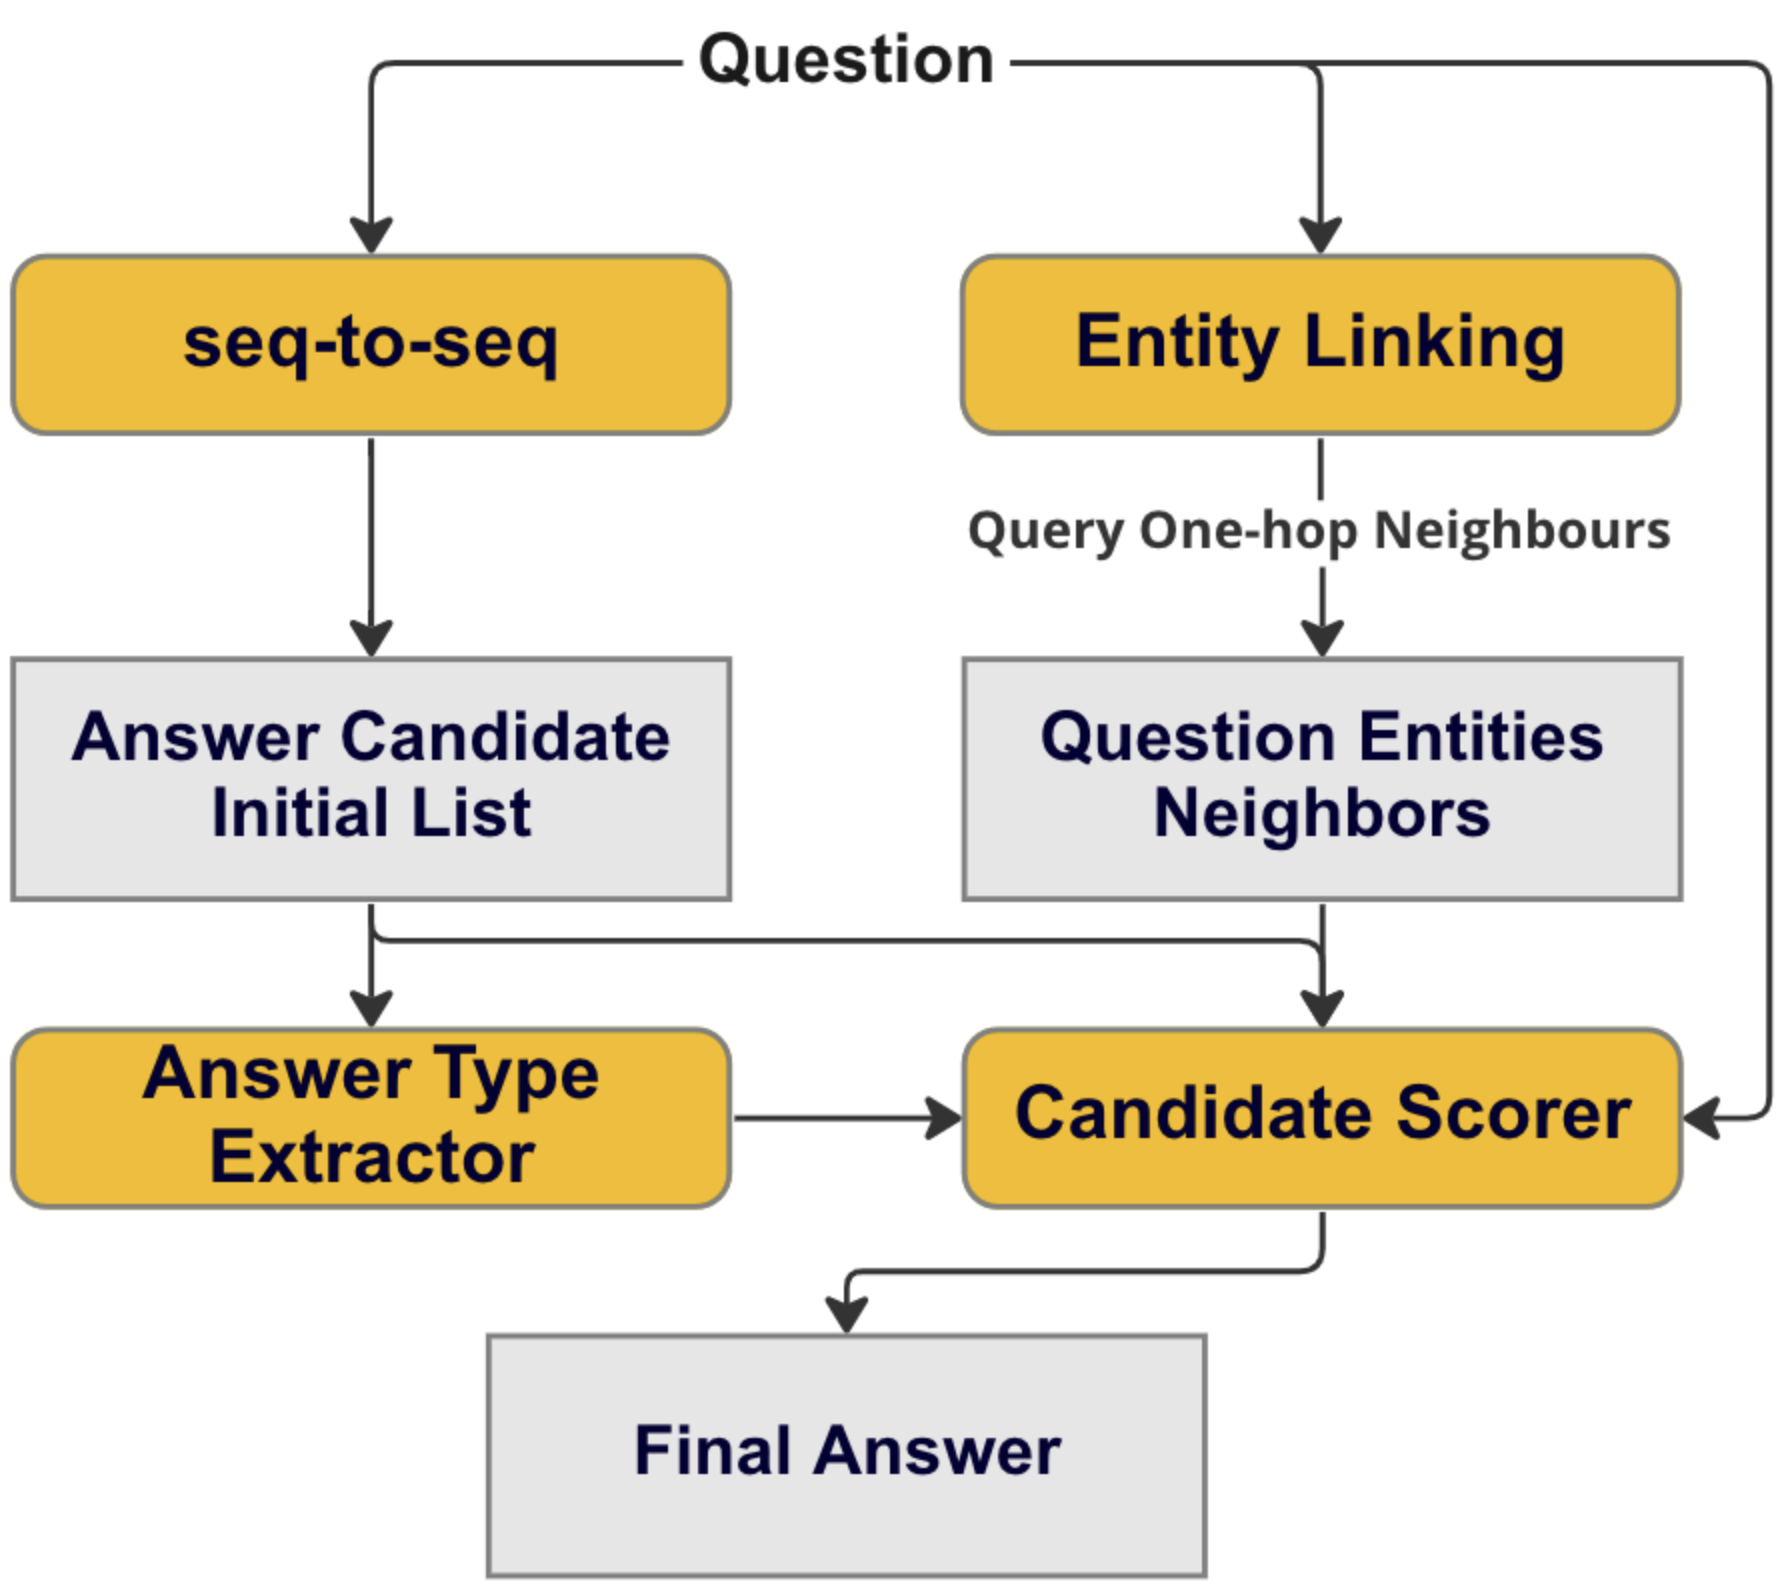
\includegraphics[width=0.85\textwidth]{act_selection/pipeline.png}
    \caption{ACT Selection Pipeline: (1) Put question to sequence to sequence language model to generate answer candidates, (2) Extract type from candidates, (3) Extract entities from the questions and query one-hop neighbors of the entities in the KG, (4) Filter candidates by type, (5) Select the best candidate.}
    \label{fig:act_selection:pipeline}
\end{figure}

\begin{figure}[htb]
    \centering
    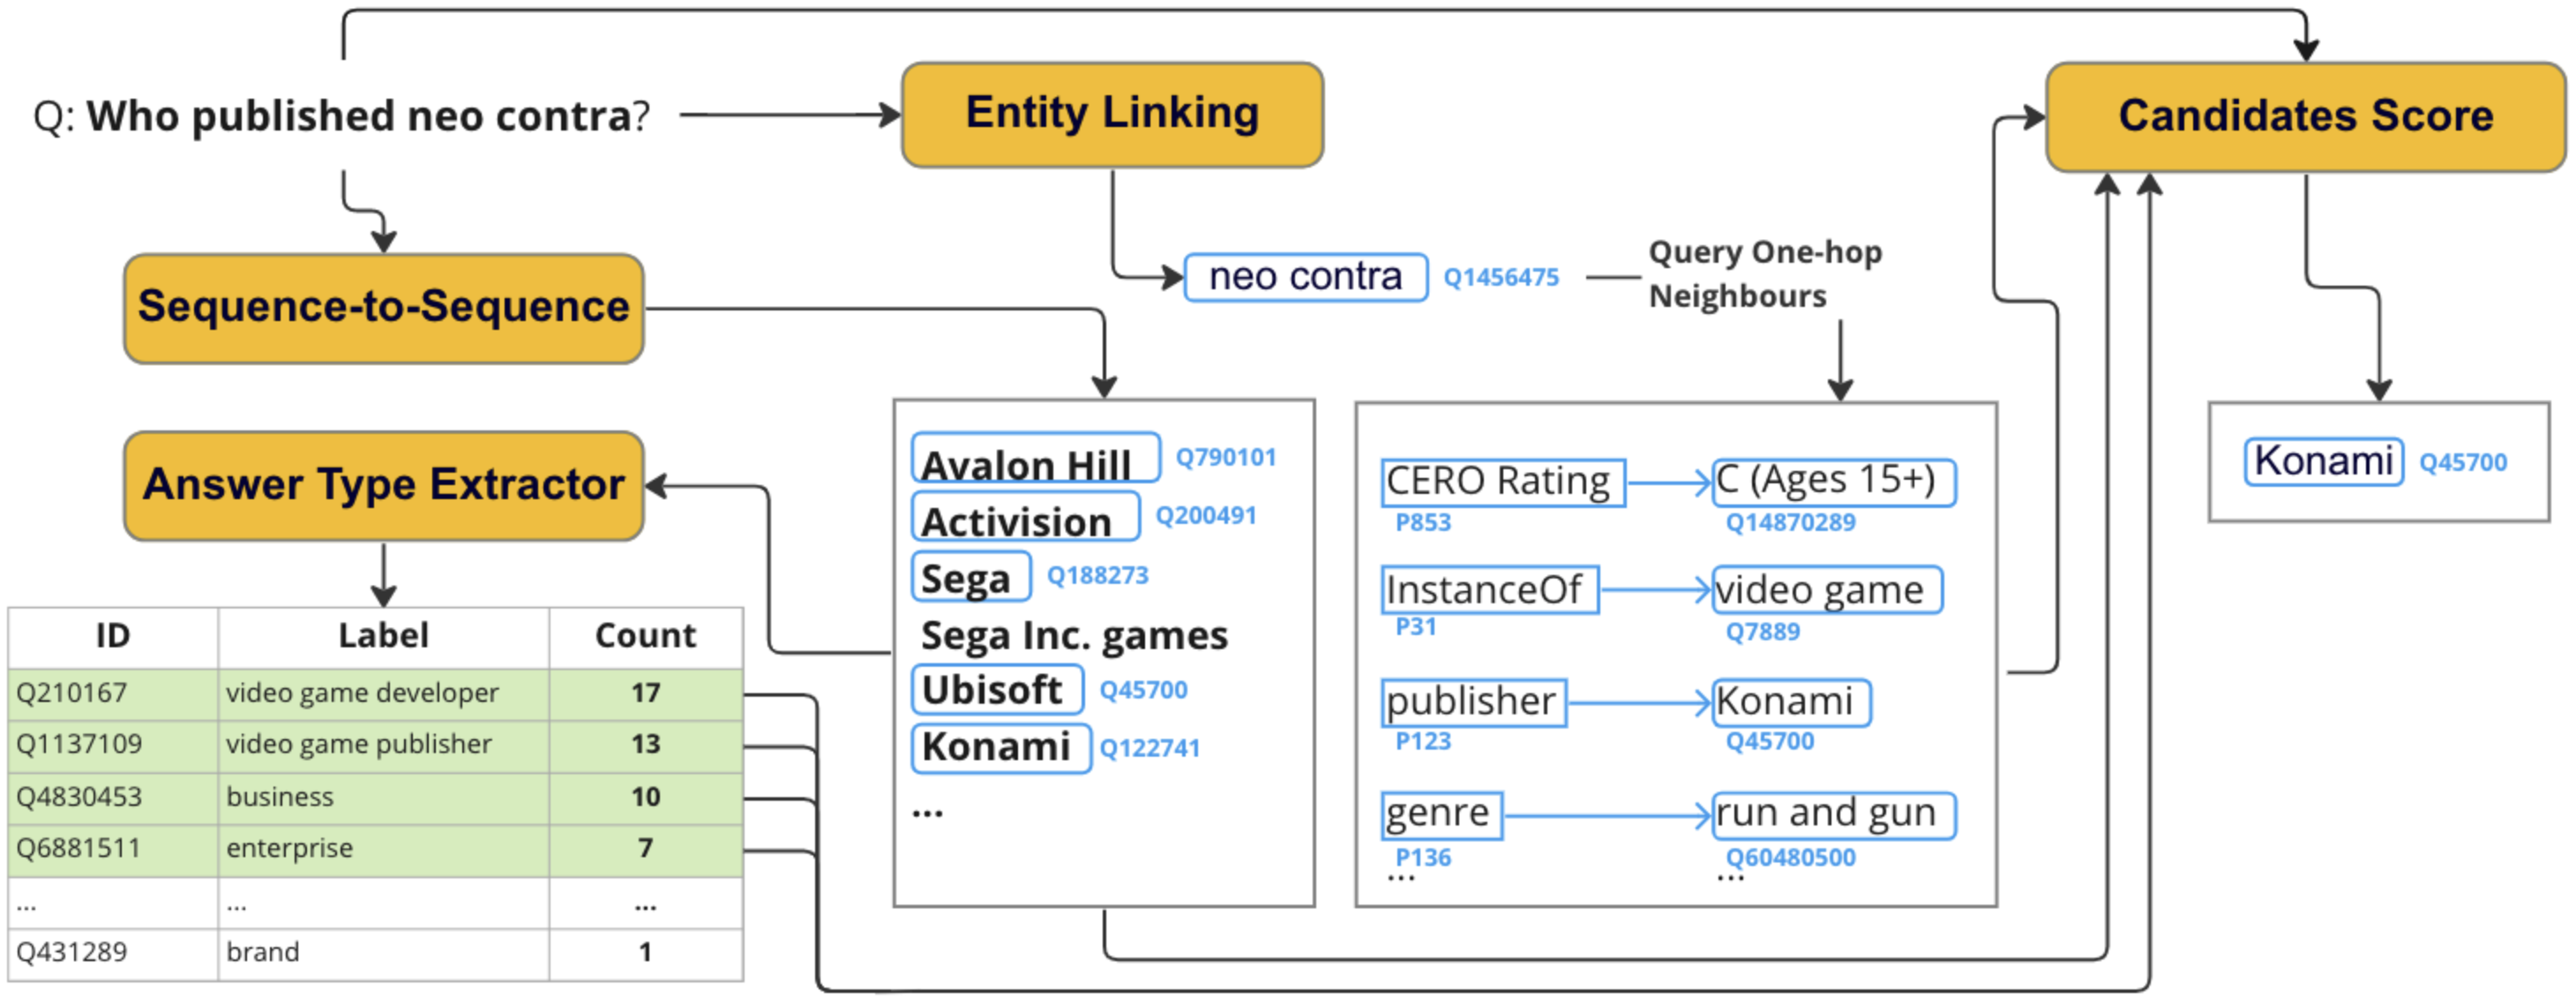
\includegraphics[width=0.95\textwidth]{act_selection/pipeline_example.png}
    \caption{The Answer Candidate Type (ACT) Selection pipeline for Knowledge Graph Question Answering (KGQA). The process combines a sequence-to-sequence model with knowledge graph-based entity linking and scoring to identify the correct answer, "Konami," as the publisher of "Neo Contra."}
    \label{fig:act_selection:pipeline_example}
\end{figure}

\section{Initial Answer Candidate Generation}
\label{sec:act_selection:initial_answer_candidate_generation}
When using \texttt{Classical Beam Search}, the output is often minor variations of a single sequence, which may not generate enough unique answer candidates for the Question Answering task. We use Diverse Beam Search~\cite{DBLP:journals/corr/VijayakumarCSSL16-diverse-beam-search} to generate an initial list of answer candidates.

The formula~\ref{eq:candidate_generation:diverse_beam_search} involves splitting the set of beams at time $t$ into $g$ disjointed subsets $Y_{[t]}^g$, and then selecting the candidate with the highest diversity penalty, which is calculated as the sum of a diversity penalty function $\Theta(y_{b,[t]}^g)$ over all candidates in the subset. Additionally, a dissimilarity term is included, which is calculated as the sum of a dissimilarity function $\Delta(y_{b,[t]}^g, Y_{[t]}^h)$ over all previous subsets $Y_{[t]}^h$ up to time $g-1$. The dissimilarity term is weighted by a parameter $\lambda_g$. This formula is used to optimize the selection of answer candidates in a computationally efficient manner.

\begin{equation}
    \begin{aligned}
        Y_{[t]}^g = \quad & \underset{y_1^{g}, \dots, y_{B\prime}^g \in Y_t^g} {\text{argmax}} \quad \underbrace{\sum_{b \in [B\prime]} \Theta(y_{b, [t]}^g)}_{\text{diversity penalty}} \\ 
        & + \underbrace{\sum_{h=1}^{g-1} \lambda_g \Delta(y_{b,[t]}^g, Y_{[t]}^h)}_{\text{dissimilarity term}},
    \end{aligned} 
    \label{eq:act_selection:diverse_beam_search}
\end{equation}

Using Diverse Beam Search instead of Greedy Search often leads to a better exploration of the search space by ensuring that alternative answers are considered.  We define the types of entities using the Wikidata property \texttt{instance\_of}~(P31). Note that an entity can be of multiple types. Finally, the initial list of answer candidates is used in the Answer Candidate Typing and the Candidate Scorer with the mined candidates. 

\subsection{Answer Candidate Typing} \label{sec:act_selection:act_typing}
We rank all types by their frequency in the initial list of answer candidates. 
After that, we merge the top-$K$ most frequent types and similar types to the final list $T$.
Types similarity is calculated as cosine similarity between Sentence-BERT~\cite{reimers-2019-sentence-bert} embeddings of respective labels. The final types are defined as the ones where similarity is greater than a threshold.

A similar aggregation method using hypernyms (also known as ''is-a''  or ''instance-of'' relations) was used in the past to label clusters of words senses in distributional models~\cite{biemann2013text}: distributionally similar words share common hypernym and top common hypernyms are surprisingly good labels for sense clusters. The analogy in our method is that language models appear to produce a list of distributionally similar candidates.

\subsection{Entity Linking}
To enrich the list of candidates, we add all one-hop neighbors of the entities found in the question. For that, we use the fine-tuned spaCy Named Entity Recognition~(NER)\footnote{\url{https://spacy.io}.}

Based on a comprehensive review of state-of-the-art Named Entity Recognition (NER) systems \cite{vajjala-balasubramaniam-2022-really}, we evaluated the top three approaches: spaCy\footnote{\url{https://spacy.io}}, Stanza\footnote{\url{https://stanfordnlp.github.io/stanza/}}, and SparkNLP\footnote{\url{https://nlp.johnsnowlabs.com}}. Our analysis revealed that pre-trained NER models performed poorly on the Simple Question Wikidata (SQWD)~\cite{SQ_WD} dataset, with entity detection failure rates ranging from 64\% to 88\%. Among these systems, spaCy demonstrated the best performance, leading us to select its standard configuration\footnote{\url{https://spacy.io/usage/training/}} for further fine-tuning. The implementation of this pipeline required two critical pre-processing steps. First, we needed to identify the entity span to feed into the algorithm. This necessitated first extracting entity labels and their corresponding redirects, then locating these labels within the question text to determine spans. For entities without exact matches in the question, we employed fuzzy search techniques\footnote{\url{https://pypi.org/project/fuzzywuzzy/}}. Second, spaCy's training process requires entity type tags (e.g., PERSON for "Elon Musk", ORG for "Tesla" - following the BIO tagging scheme), which were not provided in the original datasets. We initially assigned the PERSON tag universally across all entities. Subsequent experiments with more precise entity type tagging did not yield significant improvements.
After extensive evaluation, we ultimately selected mGENRE \cite{decao2021multilingual} as our entity linking solution, which demonstrated superior performance compared to the NER-based approaches. mGENRE functions as an end-to-end entity linking system that eliminates the need for separate entity detection and disambiguation steps. Its multilingual autoregressive entity linking capabilities provided better accuracy and robustness across diverse question formulations in our experiments, making it a practical choice for our knowledge graph question answering pipeline.

\subsection{Candidates Scorer}
Finally, we calculate four scores for each entity from the answer candidate and rank them based on the weighted sum of the scores.
The scores are as follows:
% \begin{itemize}
    % \item
    \textbf{(1)~Type score} represents the size of the intersection between the set of types extracted from the answer candidates and the selected answer types. It is weighted by the number of selected answer types: $$S_\textrm{type}~=~\frac{|\textrm{Candidates' Types} \cap T|}{|T|}.$$

    % \item
\textbf{(2)~Forward one-hop neighbors score} $S_\textrm{neighbour}$ is  assigned 1 if the candidate is among the neighbors of the question entities, and 0 otherwise.

    % \item
\textbf{(3)~Text-to-Text answer candidate score} is determined by the rank of the candidate in the initial list $C$ generated by the Text-to-Text model divided by the size of the list: $$S_\textrm{t2t}~=~\frac{C.\textsc{}{index}(\textrm{Candidate})}{|C|}.$$

    % \item
\textbf{(4)~Question-Property Similarity score} $S_\textrm{property}$ measures the cosine similarity between the embeddings of the relevant property and the entire question. We employ Sentence-BERT~\cite{reimers-2019-sentence-bert} to encode the question, following a similar approach used for the Answer Candidate Type module.
% \end{itemize}
The four scores are calculated for each entity and then are combined to generate a final score that determines the entity's ranking. The answer with the highest weighted sum of scores in the candidate list is selected as the final answer:
%
$$S_\textrm{final} = S_\textrm{type} + S_\textrm{neighbour} + S_\textrm{t2t} + S_\textrm{property}.$$

\section{Experimental Design and Baselines}
\label{sec:act_selection:experimental_design}

For our experimental setup, we fine-tuned both the Text-to-Text models and the spaCy NER models. This fine-tuning process utilized the entire training portion of their respective datasets, ensuring comprehensive exposure to the data, and involved fitting each model for eight epochs—a duration chosen to balance learning effectiveness with computational resources. To generate the initial pool of answer candidates, we employed Diverse Beam Search. This search was configured with 200 beams to ensure a wide exploration of potential candidates and a diversity penalty of 0.1 to encourage variation among the generated sequences, thus preventing the candidates from being too similar to each other. Subsequently, our Answer Candidate Typing module processed these candidates by considering the top-3 most frequent types identified within the candidate list and applying a similarity threshold of 0.6. This threshold was used for merging semantically similar types, based on Sentence-BERT embeddings, to consolidate related concepts into a coherent set of answer types.

\subsection{Datasets}
To assess the efficacy of the ACT Selection method, our evaluations were conducted on three distinct Wikidata-based datasets. A key characteristic of these datasets is their focus on 'one-hop' questions, where the answer entity is directly connected to a question entity within the Knowledge Graph by a single relational link. The specific datasets employed in our study are detailed below:
\begin{itemize}
    \item \textbf{SimpleQuestions-Wikidata (SQWD)}~\cite{SQ_WD}: This dataset is an adaptation of the original SimpleQuestions~collection~\cite{simplequestions} (which was initially developed for the now-deprecated Freebase KG~\cite{bollacker2008freebase}) for the Wikidata knowledge base. It comprises 21,957 questions.
    \item \textbf{RuBQ}~\cite{korablinov2020rubq,rybin2021rubq}: A Knowledge Graph Question Answering (KGQA) dataset that features 2,910 questions in Russian, covering a variety of types. For our experiments, their provided English translations were utilized.
    \item \textbf{Mintaka}~\cite{DBLP:conf/coling/SenAS22-mintaka}: This is a larger, multilingual KGQA dataset containing 20,000 questions of diverse types. For the purpose of our experiments, we specifically focused on its subset of \emph{generic} questions. These are questions where entities are indeed one hop away from the answer entities in Wikidata, which resulted in a working set of 1,757 English questions from this dataset.
\end{itemize}

\subsection{Evaluation}

For the evaluation of all experiments discussed in this chapter, we consistently employ the {Hits@1} metric. This metric directly measures the proportion of questions for which the top-ranked answer candidate is indeed the correct one. It serves as a primary indicator of the system's accuracy in providing the single best answer.

Formally, for a given question $q$ and its corresponding ranked list of candidate answers, where $c_1$ is the top-ranked candidate, the Hits@1 metric is defined as:

\begin{equation}
    \text{Hits@1} = \frac{1}{|Q|} \sum_{q \in Q} \mathbb{I}(c_1 = c^*)
    \label{eq:act_selection:hits_at_1}
\end{equation}

where $Q$ is the set of all questions, $c^*$ is the correct answer for question $q$, $c_1$ is the first (top-ranked) candidate answer provided by the system for question $q$, and $\mathbb{I}(\cdot)$ is the indicator function that returns 1 if the condition ($c_1 = c^*$) is true, and 0 otherwise. This metric thus quantifies the percentage of questions for which the system's top prediction is the correct answer.

Our core hypothesis is that even when a closed-book Question Answering (QA) text-to-text model fails to provide the factually correct answer, it often successfully identifies the semantic type of the expected answer. To validate this, the present study meticulously extracted answer types from the outputs generated by Text-to-Text models. These extracted types were then systematically compared against the ground-truth answer types available in the SQWD dataset. Our experimental findings are quite revealing: the fine-tuned T5-Large-SSM model, when augmented with our ACT~Selection mechanism, demonstrated an ability to accurately predict the correct answer type in an impressive \textbf{94\%} of instances. This stands in stark contrast to the baseline scenario where only \textbf{61\%} of the raw candidate answers generated by the model (without ACT Selection) shared the same type as the correct answer. This significant improvement in type prediction accuracy strongly underscored the potential of this type information, providing a clear impetus to leverage it as a critical component in enhancing the overall question-answering process.
   

% We evaluate the ACT~Selection using the Hits@1 metric. Answer Candidate Type Selection: A universal approach works with any generative Text-to-Text model. 

In our evaluations, we specifically focused on two prevalent Text-to-Text model architectures: T5 and BART. Our proposed ACT Selection approach consistently leads to improved performance across the diverse datasets previously mentioned, as indicated by the mean Hits@1 scores. The Text-to-Text models underwent a fine-tuning phase using the training splits of the SQWD dataset and the complete training split of the Mintaka dataset. Following this, their performance was rigorously evaluated on the respective test splits of SQWD, RuBQ, and Mintaka, utilizing these specifically tuned model versions.

The comprehensive results, detailed in Table~\ref{tab:act_selection:full_results}, further substantiate that the ACT Selection method consistently elevates the quality of Knowledge Graph Question Answering (KGQA) across a spectrum of Text-to-Text models. Importantly, our experiments also confirmed the versatility of our method, demonstrating its effective application even in a zero-shot learning context—that is, with Text-to-Text models that have not undergone any specific fine-tuning for the QA task. The advantages conferred by ACT Selection, particularly in terms of quality uplift, are especially pronounced when applied to smaller model architectures. For instance, the T5-large model, which contains 737 million parameters, when integrated with ACT Selection, achieves a level of performance comparable to that of the significantly larger T5-11b model, boasting 11 billion parameters. This finding is particularly noteworthy as it suggests that ACT Selection can serve as a resource-efficient strategy to substantially boost performance, an important consideration when access to extremely large-scale models or extensive computational resources for fine-tuning is constrained.


\begin{table*}[ht]
    \caption{Evaluation results on three one-hop KGQA datasets (Hits@1 scores): comparing Text-To-Text Language Model with and without our proposed ACT Selection approach in zero-shot (without tuning for QA) or tuned on SQWD or Mintaka.}
    \label{tab:act_selection:full_results}
    \centering
    \resizebox{0.99\textwidth}{!}{
    \begin{tabular}{lrrrrrrrrr}
    \hline
                 & \multicolumn{3}{c}{\textit{SimpleQuestions-Wikidata}}                                                                                                                                                           & \multicolumn{3}{c}{\textit{RuBQ (English)}}                                                                                                                                                                    & \multicolumn{3}{c}{\textit{Mintaka (one-hop, English)}}                                                                                                                                                         \\ 
                           Tuned on $\rightarrow$ & \textbf{\begin{tabular}[c]{@{}l@{}}Zero-shot\end{tabular}} & \textbf{\begin{tabular}[c]{@{}l@{}}SQWD\end{tabular}} & \textbf{\begin{tabular}[c]{@{}l@{}}Mintaka\end{tabular}} & \textbf{\begin{tabular}[c]{@{}l@{}}Zero-shot\end{tabular}} & \textbf{\begin{tabular}[c]{@{}l@{}}SQWD\end{tabular}} & \textbf{\begin{tabular}[c]{@{}l@{}}Mintaka\end{tabular}} & \textbf{\begin{tabular}[c]{@{}l@{}}Zero-shot\end{tabular}} & \textbf{\begin{tabular}[c]{@{}l@{}}SQWD\end{tabular}} & \textbf{\begin{tabular}[c]{@{}l@{}}Mintaka\end{tabular}} \\ \hline
    BART-base              & 0                                                                      & 16.54                                                            & 7.08                                                                & 0                                                                      & 5.93                                                             & 3.72                                                                & 0                                                                      & 2.06                                                             & 9.12                                                                \\ 
    Ours       & 30.38                                                                  & \textbf{42.60}                                                   & 30.70                                                               & 9.50                                                                   & 11.65                                                            & \textbf{11.72}                                                      & 4.70                                                                   & 5.88                                                             & \textbf{10.29}                                                      \\ \hline
    BART-large             & 0                                                                      & 16.97                                                            & 3.02                                                                & 0                                                                      & 4.07                                                             & 4.86                                                                & 0                                                                      & 1.76                                                             & 12.65                                                               \\ 
    Ours      & 30.42                                                                  & \textbf{42.64}                                                   & 31.39                                                               & 9.50                                                                   & 12.15                                                            & \textbf{12.79}                                                      & 4.41                                                                   & 5.29                                                             & \textbf{15.29}                                                      \\ \hline
    T5-base                & 0                                                                      & 21.26                                                            & 6.19                                                                & 0                                                                      & 6.22                                                             & 6.93                                                                & 0                                                                      & 4.41                                                             & 8.24                                                                \\
    Ours        & 30.47                                                                  & \textbf{43.13}                                                   & 34.60                                                               & 9.44                                                                   & 14.44                                                            & \textbf{16.58}                                                      & 4.71                                                                   & 8.53                                                             & \textbf{10.59}                                                      \\ \hline
    T5-large               & 0                                                                      & 22.36                                                            & 9.43                                                                & 0                                                                      & 11.15                                                            & 12.15                                                               & 0                                                                      & 7.06                                                             & 14.41                                                               \\ 
    Ours       & 29.88                                                                  & \textbf{43.05}                                                   & 36.89                                                               & 9.44                                                                   & 18.94                                                            & \textbf{20.51}                                                      & 4.71                                                                   & 10.00                                                            & \textbf{15.88}                                                      \\ \hline
    T5-large-ssm           & 0.57                                                                   & 23.66                                                            & 5.92                                                                & 0.42                                                                   & 21.44                                                            & 23.87                                                               & 0.50                                                                   & 19.71                                                            & 27.65                                                               \\ 
    Ours    & 23.39                                                                  & \textbf{47.42}                                                   & 36.54                                                               & 9.72                                                                   & 26.02                                                            & \textbf{27.88}                                                      & 6.76                                                                   & 18.53                                                            & \textbf{28.24}                                                      \\ \hline
    T5-large-ssm-nq        & 5.12                                                                   & 22.52                                                            & 4.34                                                                & 18.87                                                                  & 17.80                                                            & 19.23                                                               & 17.65                                                                  & 14.12                                                            & 23.24                                                               \\ 
    Ours & 35.09                                                                  & \textbf{43.88}                                                   & 36.39                                                               & \textbf{27.52}                                                         & 25.38                                                            & 26.38                                                               & 22.94                                                                  & 14.12                                                            & \textbf{25.59}                                                      \\ \hline
    T5-11b-ssm             & 1.81                                                                   & ---                                                              & ---                                                                 & 14.09                                                                  & ---                                                              & ---                                                                 & 20.88                                                                  & ---                                                              & ---                                                                 \\ 
    Ours      & \textbf{25.84}                                                         & ---                                                              & ---                                                                 & \textbf{20.94}                                                         & ---                                                              & ---                                                                 & \textbf{24.71}                                                         & ---                                                              & ---                                                                 \\ \hline
    T5-11b-ssm-nq          & 10.94                                                                  & ---                                                              & ---                                                                 & 33.38                                                                  & ---                                                              & ---                                                                 & 41.76                                                                  & ---                                                              & ---                                                                 \\ 
    Ours  & \textbf{38.51}                                                         & ---                                                              & ---                                                                 & \textbf{38.31}                                                         & ---                                                              & ---                                                                 & \textbf{45.00}                                                         & ---                                                              & ---                                                                 \\ \hline
    \end{tabular}
    }
\end{table*}


Consistent with general observations in the field, larger models typically demonstrate superior performance. Within our experiments, T5 models, when enhanced by our suggested method, generally outperformed their BART counterparts. Crucially, however, across all evaluated T5 and BART models, the integration of ACT Selection resulted in a marked and consistent enhancement of the foundational Text-to-Text model's performance.

Finally, Table~\ref{tab:act_selection:comparsion_hits1_sqwd} showcases a performance comparison between our suggested method and prominent KGQA systems. These include QAnswer~\cite{diefenbach2020towards}, a multilingual system that operates by transforming natural language questions into SPARQL queries; KEQA~\cite{Huang2019KnowledgeGE}, which leverages 200-dimensional TransE embeddings trained on Wikidata via the Pytorch-BigGraph~(PTBG) framework~\cite{pbg}; and ChatGPT,\footnote{\url{https://openai.com/blog/chatgpt}} the widely recognized conversational AI model launched in late 2022 which has garnered significant global attention. To effectively evaluate ChatGPT's performance in this KGQA context and ensure comparability with other systems, specific methodologies were adopted for processing its outputs. For the crucial step of linking its textual predictions to structured entities within Wikidata, we utilized the full-text search capabilities offered by the Wikidata API\footnote{\url{https://www.wikidata.org/w/api.php}}. Additionally, a minor but necessary pre-processing step for answers generated by ChatGPT was the removal of any trailing dots from its predictions (e.g., transforming a response like `Yes.' to simply `Yes'). In the specific case of the RuBQ dataset, the evaluation involved verifying if the entity predicted by ChatGPT was present among the known set of possible correct answers.

Furthermore, to guide ChatGPT towards generating answers in a style that is amenable to standard KGQA evaluation protocols, we experimented with different prompting strategies. For the SQWD dataset, the prompt employed was: `Answer as briefly as possible without additional information.' A slightly more nuanced prompt was used for the RuBQ dataset: `Answer as briefly as possible. The answer should be `Yes', `No' or a number if I am asking for a quantity of something, if possible, otherwise just a few words.' These tailored prompts were designed to encourage responses that could be more directly and reliably evaluated against the ground truth answers in their respective datasets.

\begin{table}
\caption{Comparsion of the ACT Selection with KGQA baselines in terms of Hits@1 for SimpleQuestion-Wikidata (SQWD) with T5-Large-ssm fine-tuned on its training part and T5-11b-ssm-nq in zero-shot mode.}
\label{tab:act_selection:comparsion_hits1_sqwd}
\centering
    \begin{tabular}{lcc}
    \hline
    Model & SQWD & RuBQ en \\
    \hline
    QAnswer & 33.31 & 32.30 \\
    KEQA TransE PTBG & \textbf{48.89} & 33.80 \\
    % MEKER TransE PTBQ & 53.50 & 49.50 \\
    ChatGPT & 15.32 & 36.53 \\ \hline
    T5-Large-ssm (fine-tuned) & 23.66 & 21.44 \\ 
    \text{Ours}: T5-Large-ssm (fine-tuned) & 47.42 & 26.02 \\ \hline 
    T5-11b-ssm-nq (zero-shot) & 10.94 & 33.38 \\
    \text{Ours}: T5-11b-ssm-nq (zero-shot) & 38.51 & \textbf{38.31} \\
    \hline
    \end{tabular}
\end{table}

\subsection{Ablation Study and Error Analysis}
\label{sec:act_selection:ablation_study}

To gain deeper insights into the individual contributions of the different components within our ACT Selection framework, we conducted a comprehensive ablation study. The detailed results of this study are presented in Table~\ref{tab:act_selection:ablation_study}. A primary objective was to meticulously investigate the impact of each proposed scoring mechanism on the overall candidate set collection and ranking process. Crucially, we aimed to empirically confirm our hypothesis that the integration of semantic type information significantly enhances the quality of candidate selection. Our observations from this study revealed that approaches which relied solely on individual scores, such as the Question-Property Similarity score alone, did not achieve the same level of effectiveness as the complete ACT~Selection methodology which combines multiple signals.

Furthermore, this ablation study also allowed us to scrutinize the importance of the initial answer candidates generated by the Text-to-Text model. We specifically examined whether a strategy restricted to only the one-hop neighbors of question entities would be sufficient for achieving high performance. This part of the investigation was designed to quantify the distinct value added by the initial, broader set of candidates derived from the language model in the final answer selection pipeline.

\begin{table*}[ht]
\caption{Detailed results of the ablation study for the Answer Candidate Type (ACT) Selection framework. The table reports Hits@1 scores on the SimpleQuestions-Wikidata (SQWD) dataset, using the T5-large-ssm model fine-tuned specifically on SQWD. Each row investigates the performance when using different sources for answer candidates: (1) only initial candidates generated by the Text-to-Text model, (2) only candidates derived from the one-hop neighbors of question entities in the Knowledge Graph, and (3) the full set combining both sources. The columns evaluate the impact of relying on individual scoring components (Type score, Forward one-hop neighbors score, Text-to-Text LM candidates score, Question-Property Similarity score) versus the full ACT Selection approach that utilizes all scores in conjunction.}
\label{tab:act_selection:ablation_study}
    \centering
    \resizebox{\textwidth}{!}{
        \begin{tabular}{lrrrrr}
            \toprule
            & \textbf{Type score} & \textbf{\makecell{Forward one-hop\\neighbours score}} & \textbf{\makecell{Text-to-Text LM\\candidates score}} & \textbf{\makecell{Question-Property\\Similarity score}} & \textbf{All scores} \\
            \midrule
            \makecell[l]{Only initial candidates\\generated by Text-to-Text} & 2.51 & 31.73 & 27.04 & 31.82 & 35.89 \\
            \hline
            \makecell[l]{Only question\\neighbours candidates} & 5.07 & 4.84 & 4.52 & 29.86 & 30.06 \\
            \hline
            \makecell[l]{Full answer\\candidates set} & 2.81 & 5.46 & 27.04 & 30.75 & \textbf{47.42} \\
            \bottomrule
        \end{tabular}
    }
\end{table*}

Beyond the ablation study, we also performed an error analysis to further illustrate the corrective capabilities of the ACT~Selection approach, particularly in instances where the baseline Text-to-Text Language Models (LMs) initially produced incorrect answers. This analysis was conducted using a representative subset of questions and their corresponding predictions from the T5-Large-SSM model on the SQWD dataset. Our specific focus was directed towards those questions for which the model's original top-1 prediction was erroneous, yet the ACT~Selection framework successfully identified and promoted the correct answer.

Within this chosen subset of challenging questions, the standalone Text-to-Text model managed to generate the correct answer in only 58.4\% of cases. In contrast, our Entity Linking module demonstrated high efficacy, correctly extracting 99.11\% of the relevant question entities for this same subset. This highlights that the subsequent step of augmenting the candidate pool with additional candidates retrieved from the one-hop neighbors of these accurately linked question entities proved to be a crucial factor in ultimately locating and selecting the correct answer.


\section{ACT Selection Conclusion}
\label{sec:act_selection:conclusion}

In this chapter, we introduced and detailed the Answer Candidate Type~(ACT) Selection method, an approach designed to enhance question answering over Knowledge Graphs by systematically post-processing the beam-search outputs generated by Text-to-Text language models. The core of this technique lies in a straightforward yet effective aggregation of a Knowledge Graph's `instance-of` relations (such as Wikidata's P31 property). This aggregation allows for the derivation of the likely semantic type of the expected answer, which then serves as a powerful constraint for refining the candidate pool.

Our extensive experiments, conducted across three distinct English one-hop KGQA datasets, demonstrated that this relatively simple type-driven post-processing consistently improves the performance of a variety of Text-to-Text LMs. Notably, the ACT Selection method not only boosts the results of these foundational models but also compares favorably against both specialized KGQA techniques and the more recent capabilities of large conversational models like ChatGPT, even when the latter is guided by carefully selected prompts and its output is meticulously entity-linked. The robustness of this approach was evident across different scenarios, including both fine-tuned and zero-shot learning settings, underscoring its broad applicability.

Beyond its immediate application to single-relation KGQA, the ACT Selection method also holds promise for directly performing answer typing as a standalone task. Looking ahead, the principles underlying this approach could potentially be adapted to more complex scenarios, including multilingual question answering and multi-hop reasoning over KGs. Furthermore, our findings indicate a positive correlation between the size of the underlying pre-trained language model and the ultimate QA quality achieved with ACT Selection, suggesting that leveraging even larger models could lead to further significant performance gains in future work.


         
\chapter{Controllable Fusion Large Language Models and Knowledge Graphs}
\label{chap:controllable_fusion}

% Comment: This chapter focuses on the methodology for controllable fusion using KG paths

While constraining the answer type, as discussed in Chapter~\ref{chap:act_selection}, provides a valuable signal for improving factuality, another powerful approach involves leveraging the explicit relational structure within the Knowledge Graph more directly. This chapter introduces methods based on the core idea of using KG subgraphs - a small part of the KG that contains the entities from the question, answer candidate generated by the LLM, and the shortest paths between them, drawing upon the work presented in \cite{DBLP:journals/corr/abs-2310-02166, salnikovreranking} and subsequent refinements focused on reranking.


The central motivation for this chapter is to move beyond the knowledge concentrated in parameters of the LLM and instead use pathes derived from the Knowledge Graph. This is similar to how people search in knowledge graphs: they go step-by-step, or hop-by-hop, through connected entities to find answer and become sure that entities are really related. Instead of only using LLM's not transparent generation process for factuality, we suggest using the paths that connect entities from question to potential answer entities in the KG. Such paths are good indicator of factual correctness, giving more control and interpretability, because KG path itself gives concrete evidence that supports given answer.

The general pipeline for this fusion strategy, illustrated in Figure~\ref{fig:controllable_fusion:big_pipe}, involves several stages. First, relevant entities are identified within the input question. Second, candidate answers might be generated by an LLM, or potential answer entities are retrieved from the KG, focusing on entities connected to the question entities via relatively short paths. Crucially, features are extracted from these connecting paths (or the surrounding subgraph). These features capture information about the path structure and relations involved. Finally, these subgraph based features are used by a scoring or reranking model to evaluate the correctness of each candidate answer, ultimately selecting the answer best supported by the explicit structure of the Knowledge Graph. This chapter will detail the specific mechanisms developed for implementing this subgraph based fusion method.

\begin{figure}[htb]
    \centering
    \includegraphics[width=\columnwidth]{kg_path_fusion/new_paper_big_pipeline.pdf}
    \caption{The proposed method for reranking language model answers with KGs. The method includes subgraph extraction, features extraction, and various ranker approaches.}
    \label{fig:controllable_fusion:big_pipe}    
\end{figure}

\section{Answer Candidate Generation}
\label{sec:controllable_fusion:answer_candidate_generation}

As the subgraph extraction protocol requires answer candidates, we need a source of distinct answer candidates for each question, but most LLM approaches for QA, such as the one presented by \cite{DBLP:conf/coling/SenAS22-mintaka}, typically use \texttt{Greed Search} and evaluate the top-1 answer, it is important to note that the correct answer may not always be the top candidate. For example, the fine-tuned T5-XL-SSM~\cite{DBLP:conf/emnlp/RobertsRS20} model achieved higher Mean Reciprocal Rank (MRR) scores for our task, indicating that re-ranking could improve the top-1 results. 

Similar to the previous discussed method in Section~\ref{sec:act_selection:initial_answer_candidate_generation} to generate initial answer candidates, we use Diverse Beam Search~\cite{DBLP:journals/corr/VijayakumarCSSL16-diverse-beam-search} to generate an initial list of answer candidates. This candidates will be used for subgraph extraction and features extraction to rank them and get the final answer for the questions.
  
% In this section, we examine each component of the process in detail.
%  Firstly, we generate answer candidates using various LLMs and generate subgraphs, as discussed in Subsection~\ref{sec:subgraph_extract}. Next, in Subsection~\ref{sec:subgraph_features}, we will look at which attributes are used to rank responses.


% We apply {Diverse Beam Search} to the following LLMs: {T5-large-ssm}, {T5-XL-ssm}, {Mistral}, and {Mixtral} with $200$ beams, $20$ beam groups, and a $0.1$ diversity penalty. We extend our previous research~\cite{DBLP:conf/paclic/SalnikovLRNBMP23-originalpaper} by fine-tuning the proposed T5-like models and comparing them to more recent state-of-the-art models like Mistral and Mixtral, which should make our research more applicable to real-world use cases. T5-large-SSM and T5-XL-SSM were reported to be state-of-the-art both in the original Mintaka paper and our previous work, serving as a good baseline for comparison in this study.

% To finetune the T5-like models, we first train them on English questions for $10000$ steps, following the protocols outlined in the original Mintaka paper~\cite{DBLP:conf/coling/SenAS22-mintaka}. For the more state-of-the-art Mistral and Mixtral, we finetune with LoRA and train on English questions by generating the answer candidates with ``\textit{Answer as briefly as possible without additional information. [Question]}''. However, for the T5-like models, despite adhering to these protocols, we could not achieve the reported Hits@1 accuracy in the original paper. Despite this challenge, the main focus of the study is on the reranking aspect of the pipeline. Therefore, this paper's primary contribution is improving our fine-tuned models.

\section{Subgraph Extraction}
\label{sec:controllable_fusion:subgraph_extract}
The main backbone of our approach is the procedure of subgraph extraction. We rely on the information conveyed in the relationships between question-answer pairs to improve the reranking of LLM generations. To further investigate how this relationship can improve performance, we employ a subgraph extraction algorithm that generates a KG's subgraph containing entities relevant to each question-answer pair and the shortest paths between them that contain relevant properties/relationships. 
% We extract various features that can be used for reranking in addition to the subgraphs. This section presents the subgraph extraction algorithm, the features derived from the subgraphs, and our reranking approaches.

\begin{figure}[htb]
    \centering
    \includegraphics[width=\columnwidth]{kg_path_fusion/ssp_to_sub.pdf}
    \caption{The proposed method for reranking language model answers with KGs. The method includes subgraph extraction, features extraction, and various ranker approaches.}
    \label{fig:controllable_fusion:subgraph_construction_example}
\end{figure}

For each question-answer candidate pair, the desired subgraph $G$ is mathematically defined as an induced subgraph of the Knowledge Graph. Thus, given our shortest paths from $e_i~\rightarrow~A$, where $e_i$ - entity extracted from question and $A$ - Answer. We can use the following Listing~\ref{alg:controllable_fusion:sub_extract} to extract $G$. Let us define $H$ as the set of all distinct nodes within our shortest paths $P_i$. We want to preserve all edges between the nodes within $H$. For all question-answer pairs, our objective is to retain the relationship between our question entities $E$ and answer candidate entity $A_i$. The process is schematically depicted at Figure~\ref{fig:controllable_fusion:subgraph_construction_example}.

\begin{ListingEnv}[p]
    \centering % Center the listing if desired
    \caption{Subgraph Extraction Algorithm} 
    \label{alg:controllable_fusion:sub_extract} 
    \begin{lstlisting}[basicstyle=\fontsize{10pt}{12pt}\selectfont\ttfamily] % Smaller font for code Require: entities, candidate

paths = []
For entity in entities:
    shortest_paths = get_shortest_path(entity, candidate)
    paths.extend(shortest_paths)

H = set of unique nodes in paths

G = new Graph()
Add nodes from H to G

For unique_node in H:
    unique_node_neighbors = get_neighbors(unique_node)
    For neighbor_node in unique_node_neighbors:
        If neighbor_node in H:
            Add edge (unique_node, neighbor_node) to G

Return G
    \end{lstlisting}
\end{ListingEnv}


\section{Features based on Extracted Subgraphs}
\label{sec:controllable_fusion:subgraph_features}
After extracting subgraphs for all answer candidates of our LMs, we use all possible useful features for reranking. Referring to our previous study, we mainly focused on a simple text representation of the extracted subgraphs to rank our answer candidates. Thus, in this study, we propose extracting as many useful features as possible and analyzing each feature's importance in this reranking problem. We have divided the features into the following main categories: graph, text, and Graph2Text sequence features. 

\subsection{Graph Features}
\label{sec:controllable_fusion:graph_features}
With our extracted subgraphs and their corresponding answer candidate, we seek to use the relationship from the subgraphs to classify the correct answer candidate. As the first simple baseline, we utilize graph features consisting of simple numerical subgraph statistics. We hypothesize that subgraphs with the correct answer will be less ``complex'' than subgraphs with the incorrect answer candidate. Therefore, we would want the graph features to convey the complexity of the respective subgraph. With a clear objective in mind, we experiment with the following graph features:  

\begin{itemize}
    \item \textbf{Number of nodes and edges}: basic statistics of the nodes and edges of graph $G$.
    \item \textbf{Number of cycles}: a cycle of graph $G$ is a non-empty path that starts from a given node and ends at the same node. 
    \item \textbf{Number of bridges}: a bridge of graph $G$ is an edge, where its deletion increases the number of connection components. 
    \item \textbf{Average shortest path}: the average of each shortest path between the question entity and the answer entity. 
    \item \textbf{Density}: measurement of the density of a graph, where the number of edges in a dense graph is close to the maximal number of edges (each pair of nodes is connected by an edge). The density $d$ for the graph $G$ is formulated as $d = \frac{m}{n(n-1)}$, where $n$ is the number of nodes and $m$ is the number of edges in $G$.
   \item \textbf{Katz centrality}~\cite{katz1953new}: measurement of the importance (or ``centrality'' - how ``central'' a node is in the graph) of a specific node $i$ in a graph $G$. The Katz centrality for node $i$ of graph $G$ is formulated as $x_i = \alpha \sum_{j} A_{ij} x_j + \beta$, where $A$ is the adjacency matrix of graph $G$ with eigenvalues $\lambda$, $\beta$ is the parameter that controls the initial centrality, and $\alpha < \frac{1}{\lambda_{\max}}$. 
    % \item \textbf{PageRank}~\cite{page1999pagerank}: a popular algorithm used by Google to rank web pages in the search query by counting the number and quality of links to a page to determine an estimate of its importance. In graph theory, the ``web pages'' and ``links'' are synonymous with nodes and edges. 
    \item \textbf{PageRank}~\cite{page1999pagerank} is an algorithm that ranks nodes in a graph G based on the structure of incoming links, where each node's importance is calculated as the sum of the PageRank values of nodes linking to it, weighted by their outgoing link counts.

    The PageRank formula with damping factor $d$ is:
    
    $ PR(p_i) = \frac{1-d}{N} + d\sum_{p_j \in M(p_i)} \frac{PR(p_j)}{L(p_j)} $
    
    where:
    - $p_i$ is a node in graph G
    - $M(p_i)$ is the set of nodes that link to $p_i$
    - $L(p_j)$ is the number of outbound links from node $p_j$
    - $N$ is the total number of nodes in graph G
    - $d$ is the damping factor (typically 0.85)
    
    The algorithm iteratively computes these values until convergence, with the PageRank vector representing the dominant eigenvector of the modified adjacency matrix of graph G.
\end{itemize}

\noindent We hypothesize that these features may provide ranker models with insights into the complexity of the respective subgraphs.


\subsection{Text Features}
\label{sec:controllable_fusion:text_features} 
The ablation study showcased the importance of including the question within the text representation of the subgraph. Therefore, besides the simple graph features, we want to emphasize each question/answer pair without using extracted subgraphs. Thus, the text features represent the concatenation between the question and answer, separated by a semicolon --- ``\texttt{;}''. To use this simple concatenation for all ranker approaches, we encode the string using the MPNet\footnote{\url{https://huggingface.co/sentence-transformers/all-mpnet-base-v2}} embedding model~\cite{DBLP:conf/nips/Song0QLL20}.


\subsection{Graph2Text Sequence Features}
\label{sec:controllable_fusion:g2t_seq} 
Given the vast amount of data contained in Knowledge Graphs, it is essential to convert this information into natural language to facilitate understanding and accessibility. Converting a graph into text, known as KG-to-text or Graph2Text, has demonstrated notable success in various applications~\cite{DBLP:journals/corr/abs-2309-11206}. Therefore, when generating text from a Knowledge Graph, it is crucial to analyze the underlying graph structure carefully to ensure accurate translation.

Without an obvious way of incorporating the question within the subgraphs, relying purely on the subgraphs to rerank is ineffective~\cite{DBLP:conf/paclic/SalnikovLRNBMP23-originalpaper}. Therefore, we address this issue by further exploration of different KG-to-text methods. The main objective is experimenting with various techniques to represent the extracted subgraphs more explicitly. For this type of textual feature, we researched and developed three methods for representing subgraphs as a text, including \textbf{Graph2Text Deterministic,  Graph2Text T5, and  Graph2Text GAP}.

Firstly, we employ the \textbf{Graph2Text Deterministic} approach, the most straightforward text linearization approach. In simple terms, the subgraphs are unraveled by their matrix representation. Firstly, to linearize, we convert the subgraph into its binary adjacency matrix. Let us call it matrix $A$. 
Given $n$ nodes in the subgraph, the resulting matrix's dimension will be $n \times n$. The matrix's element $[i, j]$ represents the existence of an edge between a node with index $i$ and a node with index $j$. Then, we replace the edges in the matrix with the edge label and call it $A'$. 
Adjacency matrices are typically implemented with graphs with numeric weights. The weights were string representing the relationship between our nodes. Thus, we represented the existence of an edge with $1$, then replaced in the edge with the string relationship.
%Let us call this adjacency matrix with edge information . 
Lastly, we unravel $A'$ row by row to produce our final sequence and add the triple (node\_from, edge, node\_to) to our final sequence. Listing~\ref{alg:controllable_fusion:sub2seq} summarizes the aforementioned steps. 

\begin{ListingEnv}[p]
    \centering % Center the listing if desired
    \caption{Subgraphs to Sequence - Graph2Text Deterministic} 
    \label{alg:controllable_fusion:sub2seq} 
    \begin{lstlisting}[basicstyle=\fontsize{10pt}{12pt}\selectfont\ttfamily] % Smaller font for code

Require: Subgraph G
Ensure: Text representation of subgraph Seq

adj_matrix = get_adjacency_matrix(G)
Seq = ""
# Assuming adj_matrix is n x n, where n is number of nodes
# and indices correspond to node IDs
For i in range(number_of_nodes(G)): 
    For j in range(number_of_nodes(G)):
        # Assuming 0 indicates no edge, non-zero indicates an edge
        If adj_matrix[i][j] != 0: 
            # Assuming G allows lookup by index i, j
            node_i_label = get_node_label(G, i) 
            node_j_label = get_node_label(G, j)
            # Get edge info (label/type) between node i and j
            edge_info = get_edge_info(G, i, j) 
            # Append triple to sequence string, separated by e.g., semicolon
            Seq += node_i_label + " " + edge_info + " " + node_j_label + "; " 
Return Seq
    \end{lstlisting}
\end{ListingEnv}

For the remaining two text linearization approaches, \textbf{Graph2Text T5} and \textbf{Graph2Text GAP}, we employ more complex neural-based models trained on the WebNLG~2.0 dataset~\cite{DBLP:conf/acl/GardentSNP17}. This dataset consists of instances, where each includes a Knowledge Graph from DBpedia~\cite{DBLP:conf/semweb/AuerBKLCI07} and a target text comprising one or more sentences that describe the graph. The test set is divided into partitions of seen (DBpedia categories present in the training set) and unseen (DBpedia categories not present in the training set). The statistics of this hand-crafted and human-verified dataset are described in detail in Table~\ref{tab:controllable_fusion:webnlg_label}. 

\begin{table}
    \centering
    \caption{Statistics of the WebNLG 2.0 parallel knowledge graph-to-text dataset.}
    
    \begin{subtable}[t]{0.48\textwidth}
    \centering
    \begin{tabular}{lr}
        \toprule
        \textbf{Entities} & 2,730 \\
        \textbf{Relations} & 354 \\
        \textbf{Triples} & 81,927 \\
        \bottomrule
    \end{tabular}
    \caption{Knowledge Graph statistics. Total number of KG components, number of tokens in the narratives.}
    \label{tab:kg_stats}
    \end{subtable}
    \hfill
    \begin{subtable}[t]{0.48\textwidth}
    \centering
    \begin{tabular}{lr}
        \toprule
        \textbf{Total} & 623,902 \\
        \textbf{Unique} & 8,075 \\
        \textbf{Entity} & 60\% \\
        \bottomrule
    \end{tabular}
    \caption{Texts statistics. The percentage of text entities represents the portion of the text that includes entity labels.}
    \label{tab:controllable_fusion:webnlg_label}
    \end{subtable}
\end{table}

The idea behind the \textbf{Graph2Text T5} approach is to extract informative and useful features from KGs using pre-trained text-to-text LMs. With the impressive capabilities of pretrained LMs in the text-to-text generation task, we seek to replicate such results in the graph-to-text scope. Our idea is built upon the analogous algorithm discussed in~\cite{DBLP:journals/corr/abs-2007-08426}. The authors tackle the graph-to-text generation task in this work with two popular text-to-text pre-trained LMs, BART and T5. These models have an encoder-decoder architecture, which makes them well-suited for conditional text generation tasks. To adapt these models for the graph-to-text task, the authors continue pre-training BART and T5 using the following approaches:

\begin{enumerate}
    \item Language Model Adaptation (LMA): the models are trained on reference texts that describe graphs, following the BART and T5 pre-training strategies.
    \item Supervised Task Adaptation (STA): the models are trained on pairs of graphs and their corresponding texts collected from the same or a similar domain as the target task --- graph-to-text in this case. 
\end{enumerate}

Building on the STA approach via T5 and WebNLG~2.0, we obtain graph-to-text sequences by first converting the graph into a sequence of tokens through linearization. We use the string ``convert the [graph] to [text]:'' to acquire this linearised sequence. This output sequence is then fed into the input sequence for the T5 model tuned on WebNLG~2.0. 
% For tuning Graph2Text T5 approach, we use the following hyperparameters: \textit{learning rate}: $1e^{-3}$, \textit{batch size}: 4, \textit{gradient accumulation steps}: 32, and \textit{Adam optimizer}. 

The \textbf{Graph2Text GAP} approach is based on the current state-of-the-art graph-to-text task, GAP, built on BART~\cite{DBLP:conf/coling/ColasAW22-GAP}. 
The main idea of GAP is a fully graph-aware encoding combined with the coverage of pre-trained LMs. The GAP KG-to-text framework fuses graph-aware elements into existing pre-trained LMs, capturing the advantages brought forth by both model types. The architecture of this solution consists of two main components:

\begin{enumerate}
\item \textbf{Global Attention}: to capture the graph's global semantic information, the graph's components are first encoded using an LM. This allows the model to leverage the lexical coverage of pre-trained LMs.
\item \textbf{Graph-aware Attention}: to attend to and update the representations of entities, relations, or both, a topological-aware graph attention mechanism was introduced, which includes entity and relation type encoding.
\end{enumerate}

Applying the work of GAP, we first linearize the input graph into a text string by creating a sequence of all triples in the KG, interleaved with tokens that separate each triple and the triple's components (head, relation, and tail). Then, we use a transformer encoder to obtain vector representations. The first module in each transformer layer acts as a Global Attention and captures the semantic relationships between all tokens. Moreover, we use a Graph-aware Attention module to capture the sparse nature of adjustment in a graph and apply it to entity and relation vectors from word vectors. By proposing this flexible framework, where graph-aware components can be interchanged, the current architecture aims to generate coherent and representative text descriptions of the KG. Like the Graph2Text T5 approach, we pretrain the model on the WebNLG~2.0 dataset and get the final predictions through the fine-tuned model. 
% For finetuning the Graph2text GAP approach, we use the following hyperparameters: \textit{learning rate}: $2e^{-5}$, \textit{batch size}: 16; \textit{beam size}: 5, \textit{Adam Optimizer}, 50 \textit{nodes}, and 60 \textit{relations}.


In this research, we introduce the more complex neural-based graph-to-text approach to explore further the reranking capabilities of the textual representation of our extracted subgraphs. The initial rudimentary text linearization approach has already achieved state-of-the-art Hits@1. We look for a more complete case study on reranking the text linearization with these two neural-based linearization approaches. To better understand the differences between these methods, we present several illustrative examples that demonstrate how T5 and GAP handle different types of knowledge graph structures.

Let us examine four representative examples that highlight the key differences in how these models process and represent graph information presented in on Figures~\ref{fig:controllable_fusion:g2t_example1},~\ref{fig:controllable_fusion:g2t_example2},~\ref{fig:controllable_fusion:g2t_example3}, and~\ref{fig:controllable_fusion:g2t_example4}:

\begin{figure}[!htb]
    \centering
    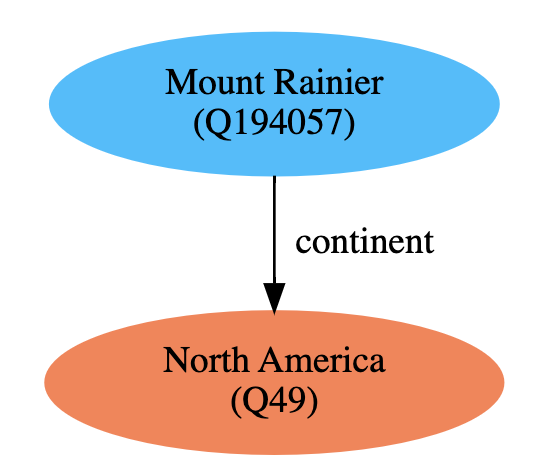
\includegraphics[width=0.5\textwidth]{kg_path_fusion/g2t_examples/g2t_e1.png}
    \caption{Example 1: Simple location relationship between Mount Rainier and North America. The T5 model correctly states ``Mount Rainier is located in North America,'' while GAP introduces an incorrect inference by stating ``The summit of North America is called Mount Rainier.''}
    \label{fig:controllable_fusion:g2t_example1}
\end{figure}

\begin{figure}[!htb]
    \centering
    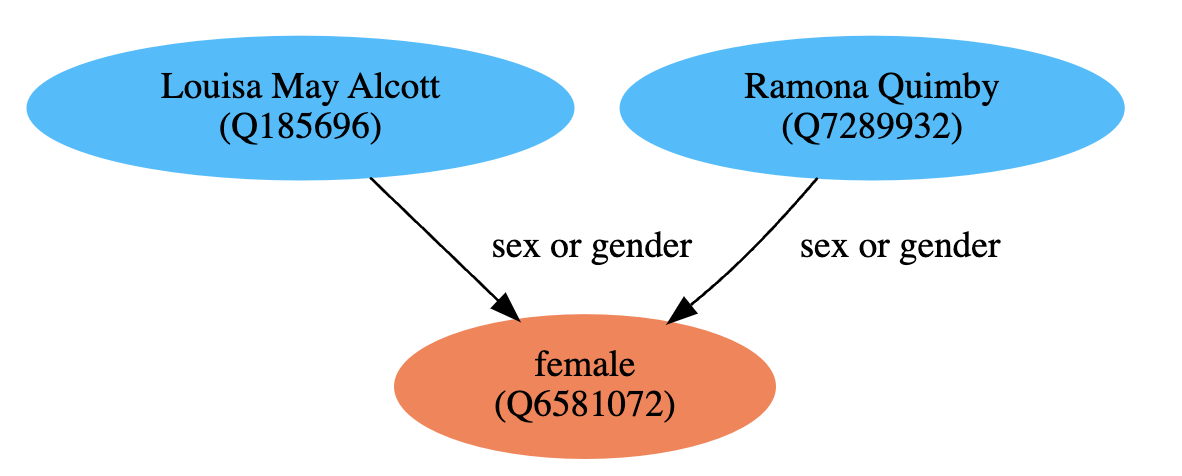
\includegraphics[width=0.6\textwidth]{kg_path_fusion/g2t_examples/g2t_e2.png}
    \caption{Example 2: Gender information for two authors. The T5 model accurately states ``Louisa May Alcott and Ramona Quimby are both females,'' while GAP makes a significant error by stating they are ``both men,'' demonstrating a critical failure in preserving factual information.}
    \label{fig:controllable_fusion:g2t_example2}
\end{figure}

\begin{figure}[!htb]
    \centering
    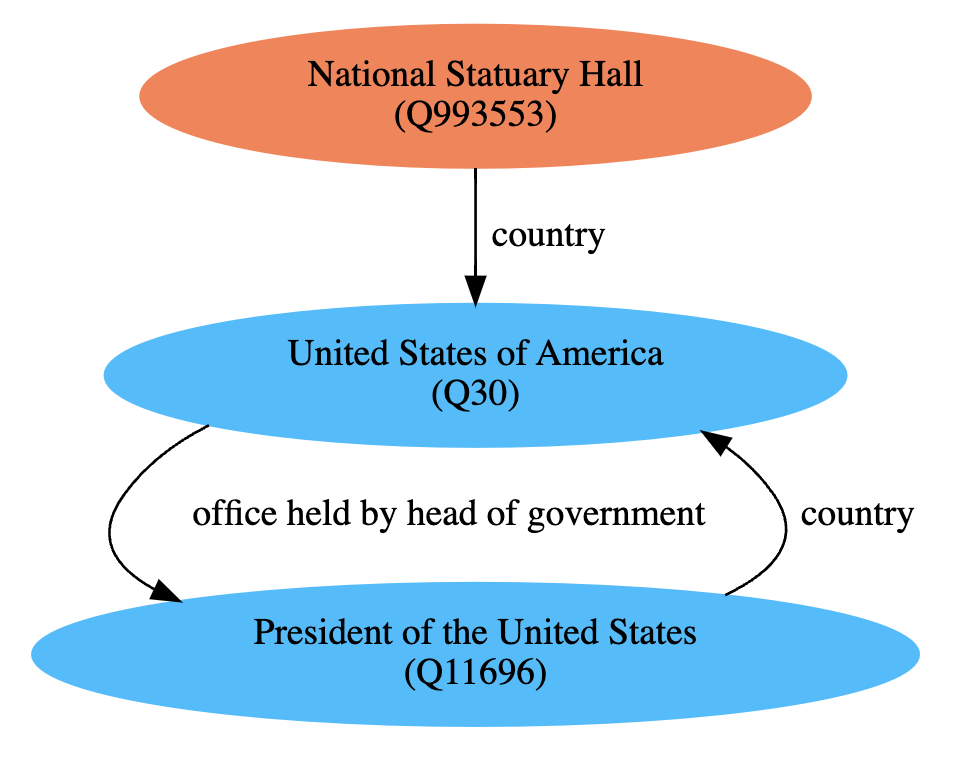
\includegraphics[width=0.6\textwidth]{kg_path_fusion/g2t_examples/g2t_e3.png}
    \caption{Example 3: Complex relationships involving the United States and its institutions. The T5 model provides a clear and accurate description: ``The United States of America is the location of the National Statuary Hall and the office of the President of the United States.'' In contrast, GAP generates a more verbose and less precise description, introducing unnecessary information about Congress and creating redundant statements about the presidency.}
    \label{fig:controllable_fusion:g2t_example3}
\end{figure}

\begin{figure}[!htb]
    \centering
    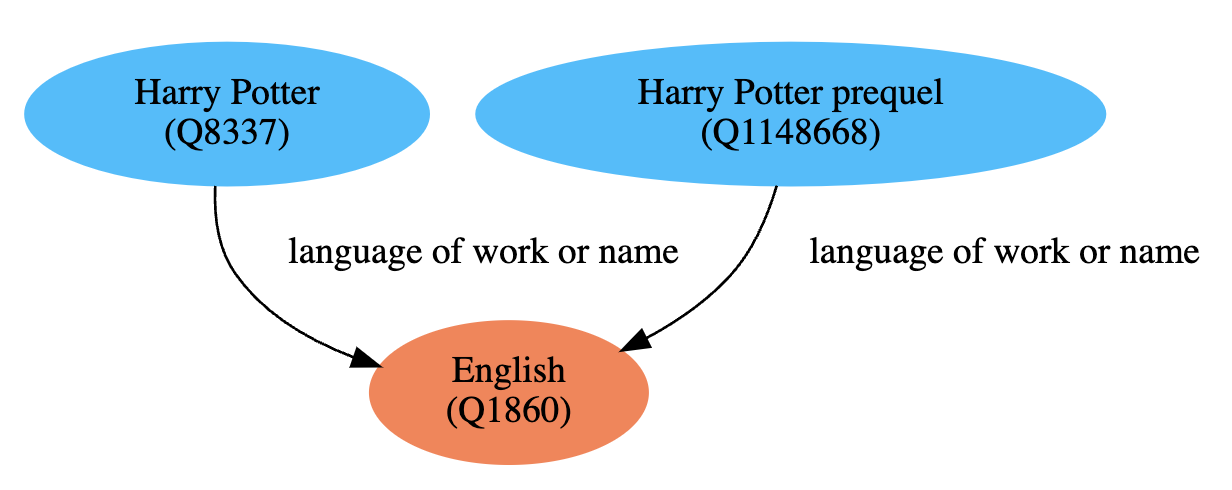
\includegraphics[width=0.6\textwidth]{kg_path_fusion/g2t_examples/g2t_e4.png}
    \caption{Example 4: Language information for Harry Potter works. The T5 model correctly states ``The Harry Potter prequel is written in English, as is the Harry Potter book,'' while GAP makes an error by referring to ``the English book'' instead of ``the Harry Potter book,'' demonstrating a tendency to lose specific entity information.}
    \label{fig:controllable_fusion:g2t_example4}
\end{figure}

These examples reveal several important patterns in how the two models handle graph-to-text conversion:

\begin{enumerate}
    \item \textbf{Factual Accuracy}: T5 consistently maintains higher factual accuracy, while GAP occasionally introduces incorrect inferences or loses specific entity information.
    
    \item \textbf{Information Preservation}: T5 better preserves the specific details from the knowledge graph, whereas GAP tends to generalize or introduce unnecessary information.
    
    \item \textbf{Conciseness}: T5 generates more concise and focused descriptions, while GAP often produces more verbose output with redundant information.
    
    \item \textbf{Entity Handling}: T5 demonstrates better handling of entity relationships, while GAP sometimes confuses or misrepresents entity attributes.
\end{enumerate}

These observations align with our quantitative findings presented in Table~\ref{tab:controllable_fusion:g2t_accuracy}, where T5 shows superior performance in preserving both question and answer entities. The examples particularly highlight GAP's tendency to introduce hallucinations and lose specific entity information, which explains its lower accuracy scores in our evaluation.

% All three variations of Graph2Text Sequence features are further encoded with the MPNet embedding model~\cite{DBLP:conf/nips/Song0QLL20}, discussed more in \ref{appx:detailed_results}. Moreover, motivated by our previous research, we employ context and highlight these Graph2Text sequences, discussed further in \ref{hl_context}.


\section{Rank LLM answer candidates using subgraphs} \label{sec:controllable_fusion:ranker}
With the subgraphs and their extracted features discussed above, we devise several reranking approaches to maximize the performance of the base large language models. As the focal point of the research is the reranking scope, we employ reranking methodologies from least to most complex. The hypothesis is a positive trend in performance as we apply more complex models and features.

As a starting point, we employ semantic reranking. This is a popular solution in information retrieval~\cite{DBLP:journals/jifs/FigueroaPP20, DBLP:journals/corr/HendersonASSLGK17}, implemented differently under the same name. Building on this foundation, our semantic ranker utilizes the MPNET~\cite{DBLP:conf/nips/Song0QLL20} embeddings of the answer candidates, further justified in~\ref{mpnet_explain}. We then rank the answer candidates by the cosine similarity between the embedding vectors. 

In the next layer of complexity, we utilize regression-based models, namely, linear and logistic regression. %~\cite{legendre1806nouvelles}
For the features set, we apply all features discussed in~\ref{sec:controllable_fusion:subgraph_features} (for features in text/string format, we apply MPNET embeddings, discussed in~\ref{mpnet_explain}). In the case of linear regression, we employ ordinary least squares linear regression to predict either $1$ or $0$, corresponding to correct and incorrect responses, respectively. The predicted score was then used to rank the potential answers by sorting the values from highest to lowest. Although we employ logistic regression for the same reranking task, we reformat the problem to a classic classification problem. We sort the answers with the highest classification confidence to rank the candidates. We use a standard logistic regression model with L2 regularisation. 

In addition to regression-based models, we want to utilize the same features with a more complex ranker. Thus, we explore and experiment with the gradient boosting model, specifically the CatBoost regression model~\cite{DBLP:conf/nips/ProkhorenkovaGV18-catboost}. Before training, we use grid search to finetune \textit{learning\_rate, depth,} and \textit{iteration}. We use root-mean-square deviation (RMSE) to evaluate. Like linear regression, we use the predicted score to rank the answer candidates by sorting the values. 

Last but not least, the most effective and complex approach for reranking answer candidates is a neural-based ranker with textual features as input. We experiment with a transformer-based model with an additional regression head layer, which is fine-tuned using {mean-square loss} and {AdamW} optimisation~\cite{DBLP:conf/iclr/LoshchilovH19-adamw}. To keep the experiments clear and transparent, we keep the same MPNet model for this ranker. We employ this variation of sentence transformer throughout this research for various sentence/text embeddings, as mentioned in~\ref{mpnet_explain}. Due to the lack of a straightforward method for utilizing numeric or table-like features with this ranker, we choose not to apply graph features. 


\section{Experiments}
In this section, we describe an experimental setup to test the usability of our proposed language model reranking methods based on KGs. We explore the impact of different combinations of features on reranking performance and examine the effects of various reranking methods, ranging from simple to more sophisticated, on reranking accuracy.

\subsection{Dataset} \label{sec:dataset}
To further enhance the results gathered in the original paper, we also conduct our research on Mintaka~\cite{DBLP:conf/coling/SenAS22-mintaka} dataset, which is a large-scale, complex and natural dataset that can be used for end-to-end question-answering models, composed of $20,000$ question-answer pairs. This dataset is annotated with Wikidata entities and comprises 8 types of complex questions. These types include: 
\begin{itemize}%[noitemsep]
    \item \textbf{Count}, e.g., Q: How many astronauts have been elected to Congress? A: 4.
    \item \textbf{Comparative}, e.g., Q: Is Mont Blanc taller than Mount Rainier? A: Yes.
    \item \textbf{Superlative}, e.g., Q: Who was the youngest tribute in the Hunger Games? A: Rue.
    \item \textbf{Ordinal}, e.g., Q: Who was the last Ptolemaic ruler of Egypt? A: Cleopatra.
    \item \textbf{Multi-hop}, e.g., Q: Who was the quarterback of the team that won Super Bowl 50? A: Peyton Manning.
    \item \textbf{Intersection}, e.g., Q: Which movie was directed by Denis Villeneuve and stars Timothee Chalamet? A: Dune.
    \item \textbf{Difference}, e.g., Q: Which Mario Kart game did Yoshi not appear in? A: Mario Kart Live: Home Circuit.
    \item \textbf{Yes/No}, e.g., Q: Has Lady Gaga ever made a song with Ariana Grande? A: Yes.
    \item \textbf{Generic}, e.g., Q: Where was Michael Phelps born? A: Baltimore, Maryland.
\end{itemize}

Factoid questions can sometimes have answers that cannot be linked to an entity in knowledge bases (count and yes/no questions). To handle this edge case in a production system, one could first train a classifier to categorize questions into three types: yes/no, count, and other. For this classification task, we train the MPNet (all-mpnet-base-v2)~\cite{DBLP:conf/nips/Song0QLL20} model using CrossEntropy loss. The training is performed over $5$ epochs on the Mintaka train split, utilizing a batch size of $32$, $500$ warm-up steps, a weight decay of $0.01$, and a learning rate of $0.00005$. To manage the training data, we employ the HuggingFace basic Trainer along with a Weighted Random Sampler. This approach achieves a balanced accuracy of \textbf{98.29\%} on the Mintaka test split.

This research centers around the reranking aspect of the pipeline, discussed in our previous research~\cite{DBLP:conf/paclic/SalnikovLRNBMP23-originalpaper}. Thus, with the question types listed above, we exclude {Yes/No} and {Count} questions. These question types offer no value information, as numbers and yes/no have no respective Wikidata entities, leading to a non-existent/impractical relationship between the question/answer pair. Thus, we deem {Yes/No} and {Count} pointless in the scope of our research. However, one could still utilize the entire pipeline to compute and evaluate the results based on the whole Mintaka dataset, including {Yes/No} and {Count}. 
% Referring to the question type classifier introduced in our original research ~\cite{DBLP:conf/paclic/SalnikovLRNBMP23-originalpaper}, this additional component allows for {Yes/No} and {Count} questions to receive special treatment.

We also compile and publish\footnote{\url{https://github.com/s-nlp/subgraph_kgqas-nlp/KGQA_Subgraphs_Ranking}} the dataset of subgraphs for the whole Mintaka dataset (for train, validation, and test splits separately). Additionally, we also publish the answer candidates generated by the base LMs. Subgraphs are collected using the process discussed in Section~\ref{sec:controllable_fusion:subgraph_extract}: we generate candidate answers, we take the true answer and the entities from the question entity neighbors as candidates, and construct subgraphs with Algorithm~\ref{alg:controllable_fusion:sub_extract}. As a result, we construct a ``correct'' subgraph containing the correct highlighted answer and several ``incorrect'' subgraphs from the incorrect candidate answers generated by the model. 
We present four versions of the dataset with subgraphs: with candidates generated by {T5-Large-SSM}, {T5-XL-SSM}, {Mistral}, and {Mixtral} models.

\subsection{Question Entities} \label{ques_ent}
Referencing the subgraph extraction protocol discussed in~\ref{sec:controllable_fusion:subgraph_extract}, we require question entities and the answer entity for each question-answer pair. Regarding the question entities, any entity linker such as {mGENRE}~\cite{decao2021multilingual} could be applied. However, with the objectives outlined above, utilizing an entity linker would derail the main focus of evaluating this reranking scope. As a result, we leverage the golden truth question entities provided by the Mintaka dataset. 

\subsection{Text Embeddings} \label{mpnet_explain}
Some features derived from the extracted subgraphs are in their natural language form (answer candidates for semantic ranker, Graph2Text sequences, and text features). Therefore, we use these features for our reranking objectives based on the MPNet embedding model~\cite{DBLP:conf/nips/Song0QLL20}. In Performance Sentence Embeddings (evaluation of the quality of the embedded sentence) and Performance Semantic Search (evaluation of the quality of the embedded search queries \& paragraph), the MPNet Embedding model outperforms 37 other sentence transformer models~\cite{reimers-2019-sentence-bert}. These models were compared by averaging the Performance Sentence Embeddings and Performance Semantic Search while considering the speed and the model size. In addition to the highest embedding performance, MPNet is relatively small while fast in training time. Moreover, this model is very popular within the HuggingFace community \footnote{\url{https://huggingface.co/sentence-transformers/all-mpnet-base-v2}}. Utilizing a well-known and widespread embedding model would enhance the aim of formulating our approach as a reranking problem motivated by end-user requirements. 

\subsection{Graph2Text with Highlight \& Context} \label{hl_context}
As mentioned in~\ref{sec:controllable_fusion:g2t_seq}, we focus on different text representations of the subgraphs to rank the respective answer candidates. 
We employ context for linearised text representation of the subgraph. This addition is a simple concatenation between the question and the linearised sequence, separated by a special token $<$/s$>$ to emphasize the question in the question-answer pairing. Moreover, the study showcased the effectiveness of highlighting~(HL) the answer candidate within the linearised sequence of the concatenation. 
The context is motivated by the assumption that the subgraph alone does not provide the necessary information to answer the question. In other words, the model cannot answer the question without it. Similarly, it is difficult to rank the answers if the model has no idea which entities in the subgraph are potential answer candidates.
% With this highlighting scheme, we increased the {Hits@1} by $2\%$, from $0.36 \rightarrow 0.38$ \cite{DBLP:conf/paclic/SalnikovLRNBMP23-originalpaper}. 
An example of such concatenation, the rank by MPNet to achieve the current state-of-the-art, is shown below:  

\begin{itemize}
    \item \textbf{Question}: Which actor was the star of Titanic and was born in Los Angeles, California?
    \item \textbf{Answer}: Leonardo DiCaprio
    \item \textbf{Sequence with HL and Context}: Which actor was the star of Titanic and was born in Los Angeles, California? $<$/s$>$ [unused1]Leonardo DiCaprio[unused2], place of birth, Los Angeles, Titanic, cast member, [unused1]Leonardo DiCaprio[unused2]
\end{itemize}

\noindent We employ a similar \textbf{HL} and \textbf{context} protocol to our three Graph2Text sequences. The objective is to assist the model in understanding the question-answer pair and the Graph2Text sequence. An example of such processing for the three sequences can be seen below:

\begin{itemize}
    \item \textbf{Question}: Which actor was the star of Titanic and was born in Los Angeles, California?
    \item \textbf{Answer}: Leonardo DiCaprio
    \item \textbf{Graph2Text Deterministic}: Which actor was the star of Titanic and was born in Los Angeles, California? $<$/s$>$ [unused1]Leonardo DiCaprio[unused2], place of birth, Los Angeles, Titanic, cast member, [unused1]Leonardo DiCaprio[unused2]
    \item \textbf{Graph2Text T5}: Which actor was the star of Titanic and was born in Los Angeles, California?$<$/s$>$ Los Angeles born [unused1]Leonardo DiCaprio [unused2], who played the role of Jack Sparrow in the film Titanic, was born in the United States.
    \item \textbf{Graph2Text GAP}: Which actor was the star of Titanic and was born in Los Angeles, California?$<$/s$>$Born in Los Angeles, the actor, [unused1]Leonardo DiCaprio [unused2], was a member of the crew of the Titanic.
\end{itemize}

\noindent It is important to note that we employ the \textbf{context} and \textbf{HL} approaches only for the MPNet approach, discussed in Section~\ref{sec:controllable_fusion:ranker}. Sensibly, the transformer-based model trained on sentences and paragraphs is adept at extracting useful information from natural texts. Thus, unlike our other proposed approaches, the MPNet approach classically only handles text embedding as input. Therefore, we utilize \textbf{context} and \textbf{HL} to give the model the best chance at extracting useful information to rank answer candidates. Other approaches, such as regression-based and gradient boosting, have various other features (i.e., graph, text, and sequence). Thus, we choose not to employ \textbf{context} and \textbf{HL} transformation for Graph2Text sequences for regression-based and gradient-boosting rankers. We discuss the pipeline for each ranker in more detail in Section~\ref{sec:controllable_fusion:experimental_pipeline}.

\subsection{Experimental Pipeline} \label{sec:controllable_fusion:experimental_pipeline}

With our two objectives of observing the effects of (1) different combinations of feature sets and (2) different reranking approaches in varying complexity, we devise our experiments for each answer candidate source (from either T5-Large-SSM, T5-XL-SSM, Mistral, or Mixtral)  as the following: 
\begin{itemize}
    \item Firstly, we will systematically evaluate each feature set derived from the extracted subgraphs. These feature sets are categorized and applied in an order of increasing complexity (let us denote them as $A, B, C$, where $A$ is the least complex and $C$ is the most complex). Each of these feature sets ($A$, then $B$, then $C$) will be provided as input to every proposed reranking model, which are also arranged from the simplest to the most sophisticated. The primary aim of this experimental stage is to meticulously observe and quantify the performance variations that arise when feature sets of escalating complexity are paired with reranking models of correspondingly increasing complexity. This will help us understand the interplay between the intricacy of features and the sophistication of the ranker.
    \item Secondly, we will investigate the effect of incrementally combining these feature sets. Again, starting with the least complex feature set and progressing to the most complex, we will supply these combinations to each reranking model (also ordered by complexity). Specifically, each ranker will first receive feature set $A$, then the combination $A+B$, and finally the comprehensive combination $A+B+C$. The purpose of this experimental branch is to ascertain how the progressive addition of more complex feature information influences the overall performance capabilities of each distinct reranking approach. We want to see if more information always leads to better results, or if there is a point of diminishing returns or even negative impact.
\end{itemize}
Through the execution of this detailed experimental pipeline, our overarching goal is to furnish a comprehensive and in-depth case study. This study will focus on the task of reranking answer candidates generated by Large Language Models, specifically examining how different reranking algorithms and feature sets, varying in their inherent complexity, contribute to the final outcome. We believe this will provide valuable insights into optimizing such reranking systems.

\subsection{Evaluation} \label{sec:controllable_fusion:evaluation}

As outlined in the experimental design described in Section~\ref{sec:controllable_fusion:experimental_pipeline}, our research involves conducting experiments with a diverse array of feature sets and various reranking models. Given that our methodology operates with a relatively small and pre-defined set of answer candidates for each question (typically generated by base Language Models), the primary evaluation objective is to rigorously assess our ability to identify the single correct answer from within this constrained list. This assessment is fundamental to determining the practical effectiveness of our reranking approach in the context of the overall question-answering task.

For the evaluation of all experiments discussed here, we consistently employ the {Hits@N} metric. The {Hits@N} metric is particularly insightful because, even in instances where the top-ranked answer (i.e., Hits@1) is not the correct one, it still enables a comprehensive understanding of the potential effectiveness of the applied reranker. Specifically, it quantifies whether the correct answer is successfully positioned within the top N candidates, thereby offering a measure of the reranker's ability to bring relevant answers closer to the forefront.

Formally, for a given question $q$ and its corresponding set of candidate answers $C = \{c_1, c_2, ..., c_n\}$, where $c_i$ represents the $i$-th candidate answer, the Hits@N metric is defined as:

\begin{equation}
    \text{Hits@N} = \frac{1}{|Q|} \sum_{q \in Q} \mathbb{I}(\text{rank}(c^*) \leq N)
\end{equation}

where $Q$ is the set of all questions, $c^*$ is the correct answer for question $q$, $\text{rank}(c^*)$ is the position of the correct answer in the ranked list of candidates, and $\mathbb{I}(\cdot)$ is the indicator function that returns 1 if the condition is true and 0 otherwise. This metric effectively measures the proportion of questions for which the correct answer appears within the top~N positions of the ranked candidate list.

To illustrate this point, consider a hypothetical scenario involving two distinct Question Answering (QA) systems, each capable of generating a list of, say, several dozen potential answers for a given query. If System A ranks the correct answer at the second position, while System B ranks it at the tenth position, the perceived utility for an end-user differs substantially. From an end-user's perspective, the system that presents the correct answer closer to the beginning of the ranked list (e.g., at the second position) is unequivocally more beneficial and user-friendly.

Consequently, given that the central focus of our research is specifically the task of reranking a pre-existing list of answer candidates, the {Hits@N} metric is an invaluable tool. It furnishes us with crucial insights into the performance nuances of each distinct feature set and reranking model, particularly in their capacity to elevate the correct answer's rank within the candidate list.

\section{Results \& Discussion}

This section provides comprehensive results and analysis showcasing the effectiveness of (1) different combinations of feature sets and (2) different ranking methods. Table \ref{tab:controllable_fusion:features_importance} shows the final Hits@1 results for all rankers with different answer candidates sources and various feature sets as input. We can observe several trends within this table. Firstly, for each feature set, the Hits@1 increases as the answer candidate source model gets more complex. For instance, for all rankers with text features as input, the Hits@1 increases gradually as we move from T5-Large-SSM $\rightarrow$ T5-XL-SSM $\rightarrow$ Mistral  $\rightarrow$ Mixtral. This behavior is observable in any feature set. This is, of course, a sensible trend as the model increases in tunable parameters and size. Furthermore, the experiment results demonstrate the importance of text features, including initial questions, which is a logical conclusion for all answer candidates' sources. 


\begin{table}[htbp]
\caption{Hits@1 performance of different feature sets (Text, Graph, and Graph2Text variants) across various reranking models (Linear Regression, Logistic Regression, CatBoost, and MPNet). Results are shown for different answer source models (T5-Large-SSM, T5-XL-SSM, Mistral, and Mixtral). All models were fine-tuned on the Mintaka training set using identical hyperparameters. The dash (--) indicates that the feature type is not applicable for the given model.}
\label{tab:controllable_fusion:features_importance}
    \resizebox{\textwidth}{!}{
        \begin{tabular}{c|l|c|c|c|c}
        \toprule
        \textbf{\makecell{Answers\\Source}}                & \textbf{Features} & \textbf{\makecell{Linear\\Regression}} & \textbf{\makecell{Logistic\\Regression}} & \textbf{CatBoost}     & \textbf{MPNet}        \\
        \midrule
        \multirow{5}{*}{\textbf{\begin{turn}{45}\makecell{T5-Large\\SSM}\end{turn}}} & Text & 0,2695 & 0,2605 & 0,2458 & 0,2620 \\ 
                                        & Graph & 0,2338 & 0,2335 & 0,1935 & -- \\ 
                                        & Graph2Text (Determ Lin) & 0,2550 & 0,2440 & 0,2405 & 0,3398 \\ 
                                        & Graph2Text (T5) & 0,2505 & 0,2313 & 0,2398 & 0,3493 \\ 
                                        & Graph2Text (GAP) & 0,2393 & 0,2925 & 0,2395 & 0,3395 \\ \hline
        \multirow{5}{*}{\textbf{\begin{turn}{45}\makecell{T5-XL\\SSM}\end{turn}}} & Text & 0,2955 & 0,2850 & 0,2593 & 0,3418 \\ 
                                        & Graph & 0,2550 & 0,2613 & 0,2760 & -- \\ 
                                        & Graph2Text (Determ Lin) & 0,2640 & 0,2598 & 0,2580 & 0,3923 \\ 
                                        & Graph2Text (T5) & 0,2593 & 0,2538 & 0,2485 & 0,3905 \\ 
                                        & Graph2Text (GAP) & 0,2563 & 0,2503 & 0,2590 & 0,3573 \\ \hline
        \multirow{5}{*}{\textbf{\begin{turn}{45}Mistral\end{turn}}} & Text & 0,4760 & 0,4730 & 0,3917 & 0,5115 \\ 
                                        & Graph & 0,3575 & 0,3558 & 0,3632 & -- \\ 
                                        & Graph2Text (Determ Lin) & 0,3960 & 0,3970 & 0,3862 & 0,5007 \\ 
                                        & Graph2Text (T5) & 0,4013 & 0,3985 & 0,4012 & 0,4965 \\ 
                                        & Graph2Text (GAP) & 0,3885 & 0,3850 & 0,3787 & 0,4917 \\ \hline
        \multirow{5}{*}{\textbf{\begin{turn}{45}Mixtral\end{turn}}} & Text & 0,4883 & 0,4853 & 0,4040 & 0,5237 \\ 
                                        & Graph & 0,3698 & 0,3680 & 0,3755 & -- \\ 
                                        & Graph2Text (Determ Lin) & 0,4083 & 0,4093 & 0,3985 & 0,5130 \\ 
                                        & Graph2Text (T5) & 0,4135 & 0,4108 & 0,3940 & 0,5087 \\ 
                                        & Graph2Text (GAP) & 0,4008 & 0,3973 & 0,3910 & 0,5040 \\ 
        \bottomrule
        \end{tabular}%
    }
\end{table}
    
Additionally, we can observe an interesting performance difference between Graph2Text T5 and GAP sequences. The counterintuitive high-quality results from these Graph2Text sequences indicate that the T5 performs better than the GAP on the downstream task. However, as discussed in Section~\ref{sec:controllable_fusion:g2t_seq}, the GAP model shows better results on the WebNLG~2.0 dataset. This finding motivates us to explore further the quality of Graph2Text models on the Mintaka dataset. To do so, we calculate the accuracy of the entity label represented from the subgraph in the generated text for our Mintaka subgraph dataset. 

This simple exploration reveals that GAP tends to omit some entities from the provided subgraph, as shown in Table~\ref{tab:controllable_fusion:g2t_accuracy}. 
Moreover, based on our subjective human assessment, GAP generates more hallucinations in the Graph2Text task, shown on Figures~\ref{fig:controllable_fusion:g2t_example1},~\ref{fig:controllable_fusion:g2t_example2},~\ref{fig:controllable_fusion:g2t_example3}, and~\ref{fig:controllable_fusion:g2t_example4}.

\begin{table}[ht]
    \caption{Graph2Text Accuracy of label generation for entities in texts generated from subgraphs.}
    \label{tab:controllable_fusion:g2t_accuracy}
    % \resizebox{\textwidth}{!}{
        \centering
        \begin{tabular}{llcc}
        \toprule
        \textbf{Answers Source} & \textbf{Dataset} &
        \multicolumn{1}{l}{\begin{tabular}[c]{@{}l@{}}Question Entities\\ Accuracy\end{tabular}} &
        \multicolumn{1}{l}{\begin{tabular}[c]{@{}l@{}}Answer Entities\\ Accuracy\end{tabular}} \\
        \midrule
        \multicolumn{4}{c}{Graph2Text (T5)} \\
        \midrule
        \multirow{2}{*}{T5-Large-SSM} & TRAIN & 0,995 & 0,833        \\
                                    & TEST  & 0,954 & \textbf{0,835} \\
        \hline
        \multirow{2}{*}{T5-XL-SSM}    & TRAIN & 0,955 & 0,827        \\
                                    & TEST  & 0,955 & 0,829          \\
        \midrule
        \multicolumn{4}{c}{Graph2Text (GAP)}                         \\
        \midrule
        \multirow{2}{*}{T5-Large-SSM} & TRAIN & 0,922 & 0,773        \\
                                    & TEST  & 0,923 & 0,776          \\
        \hline
        \multirow{2}{*}{T5-XL-SSM}    & TRAIN & 0,924 & 0,767        \\
                                    & TEST  & 0,926 & 0,77           \\
        \bottomrule
        \end{tabular}
    % }
\end{table}

\subsection{Features Importance}

In addition to analyzing the performance of neural Graph2Text sequences and the positive correlation between Hits@1 and the complexity of answer candidate LLMs, we conducted a comprehensive investigation into the effectiveness of various features extracted from the subgraphs. This analysis is particularly crucial for understanding which aspects of the knowledge graph structure contribute most significantly to the reranking process.

Firstly, we prepare graph features and MPNet embeddings of the text and G2T sequence features for the regression-based rankers as input. Without the embedding-like features, these regression-based rankers fail to achieve sufficient performance while solely on graph features, seen in table \ref{tab:controllable_fusion:features_importance}. Due to the nature of Logistic and Linear Regression, we split up the embedding-like features into individual values of separate columns. Thus, there are no trivial ways to assess the importance of the overall embeddings. Therefore, we hone in on the importance of the graph features for each answer candidate source.

For the regression-based rankers, we prepared two distinct types of input features:
\begin{enumerate}
    \item Graph-based features, which capture the structural properties of the subgraphs
    \item MPNet embeddings of text and Graph2Text sequence features, which encode the semantic information
\end{enumerate}

Our preliminary analysis revealed that regression-based rankers struggle to achieve satisfactory performance when relying solely on graph features, as evidenced in Table~\ref{tab:controllable_fusion:features_importance}. This limitation stems from the inherent nature of Logistic and Linear Regression models, which require us to split the embedding-like features into individual columns. This transformation makes it challenging to assess the importance of the embeddings as cohesive units. Therefore, we focused our analysis on quantifying the importance of graph features for each answer candidate source.

To ensure robust results, we conducted the permutation importance analysis with 10 repetitions, providing a more reliable estimate of each feature's effectiveness. The results are presented in two separate figures: Figure~\ref{fig:controllable_fusion:feature_importance_t5_large_xl} shows the analysis for T5-Large-SSM and T5-XL-SSM models, while Figure~\ref{fig:controllable_fusion:feature_importance_mistral_mixtral} presents the results for Mistral and Mixtral models.

The analysis revealed several significant patterns:

\begin{enumerate}
    \item \textbf{PageRank Dominance}: The PageRank feature emerged as the most influential factor across all models, suggesting its crucial role in determining the importance of nodes within the knowledge graph structure. This finding strongly supports the continued use of PageRank in both classical graph classification and Knowledge Graph Question Answering (KGQA) applications.
    
    \item \textbf{Structural Features}: Several other graph features demonstrated notable importance:
    \begin{itemize}
        \item Number of bridges, which indicates critical connections in the graph
        \item Node and edge counts, reflecting the complexity of the subgraph
        \item Average shortest path length between question entities and answer candidates
    \end{itemize}
    
    \item \textbf{Model-Specific Variations}: The importance of features varied significantly between the T5-based models (T5-Large-SSM and T5-XL-SSM) and the more recent models (Mistral and Mixtral). This variation suggests that different language models may benefit from different feature combinations, highlighting the need for model-specific feature selection strategies.
\end{enumerate}

These findings have important implications for future research and practical applications. The strong performance of PageRank suggests that it should be a standard component in graph-based reranking systems. Additionally, the varying importance of features across different models indicates that feature selection should be tailored to the specific characteristics of the underlying language model.

\begin{figure}[htb]
   \centering
   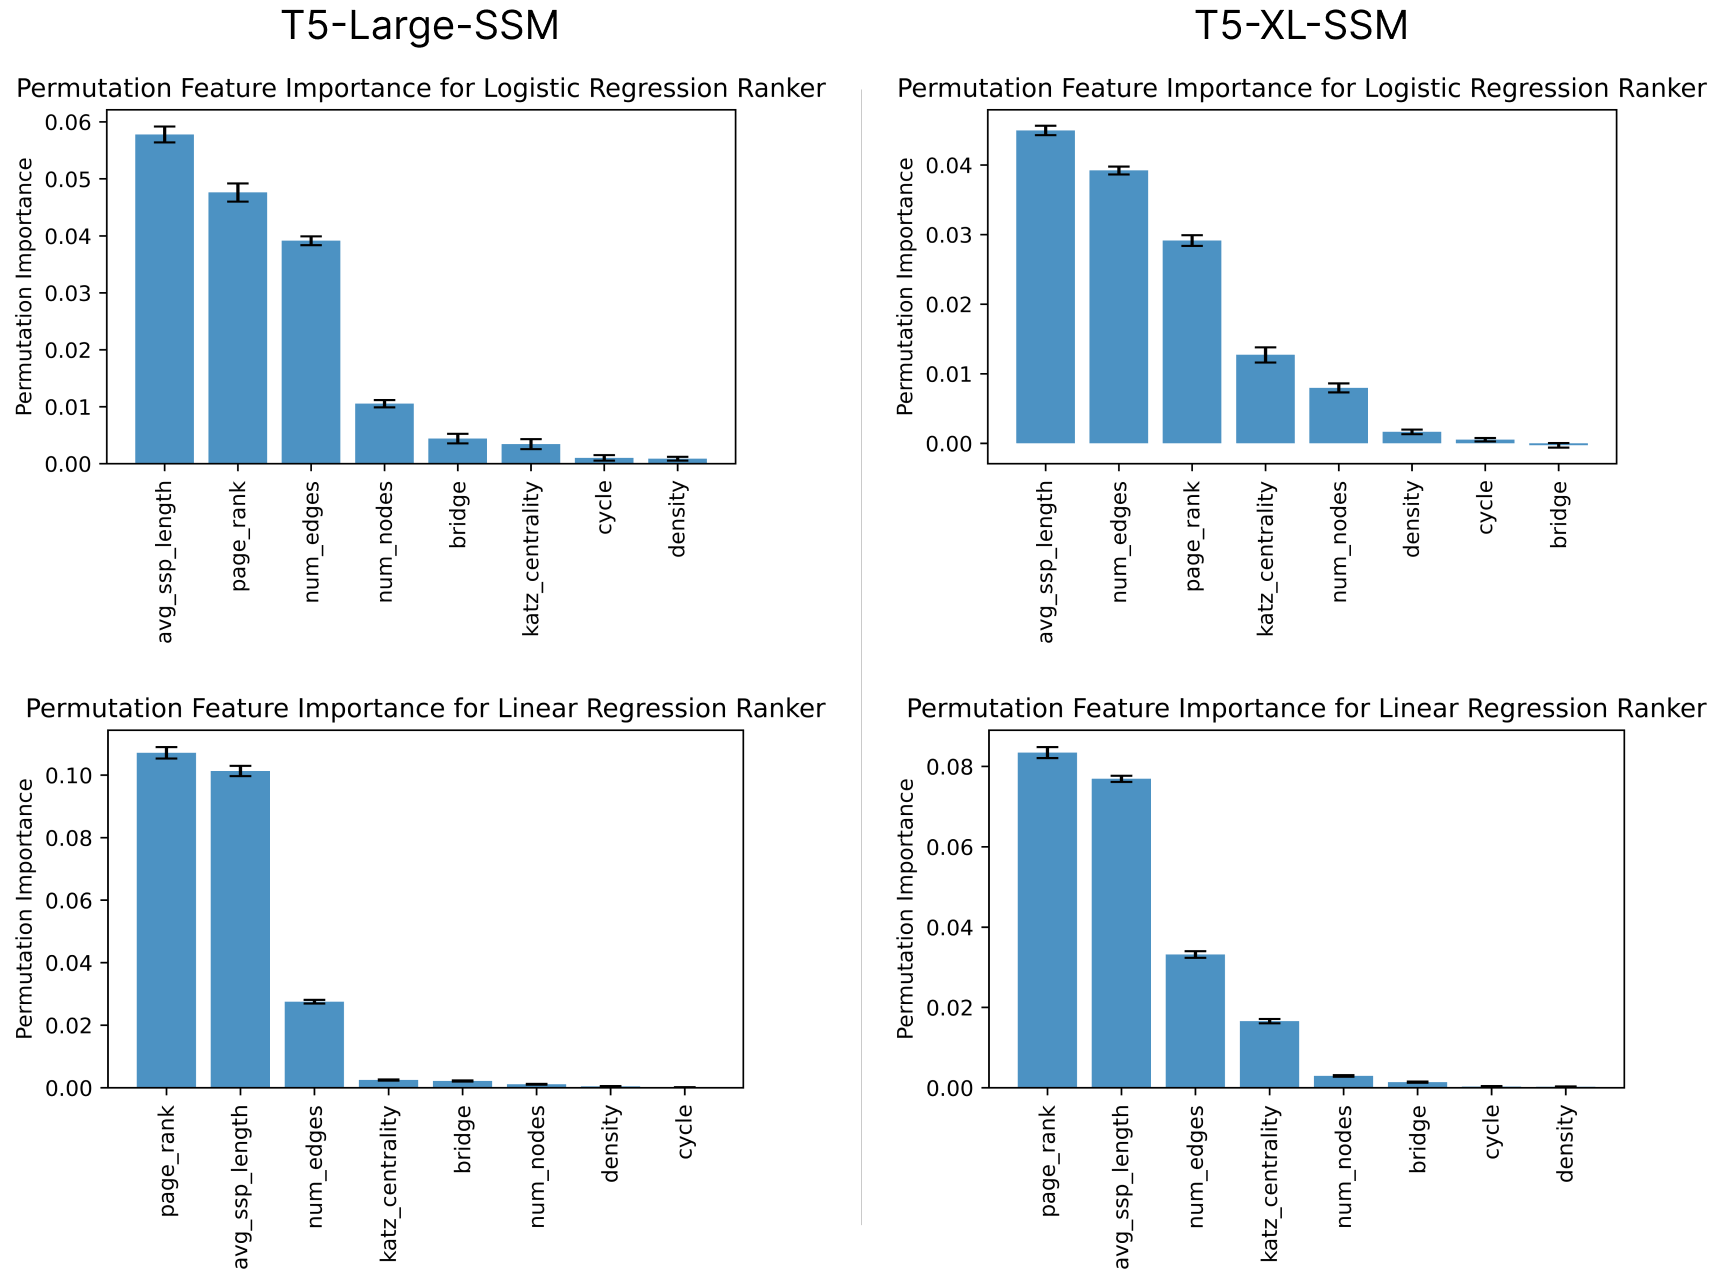
\includegraphics[width=\textwidth]{kg_path_fusion/feature_importance_t5_large_xl.png}
   \caption{Permutation importance of graph features for Linear and Logistic Regression rankers on answer candidates generated by T5-Large-SSM and T5-XL-SSM. The analysis reveals the relative contribution of each feature to the model's performance.}
   \label{fig:controllable_fusion:feature_importance_t5_large_xl}
\end{figure}

\begin{figure}[htb]
   \centering
   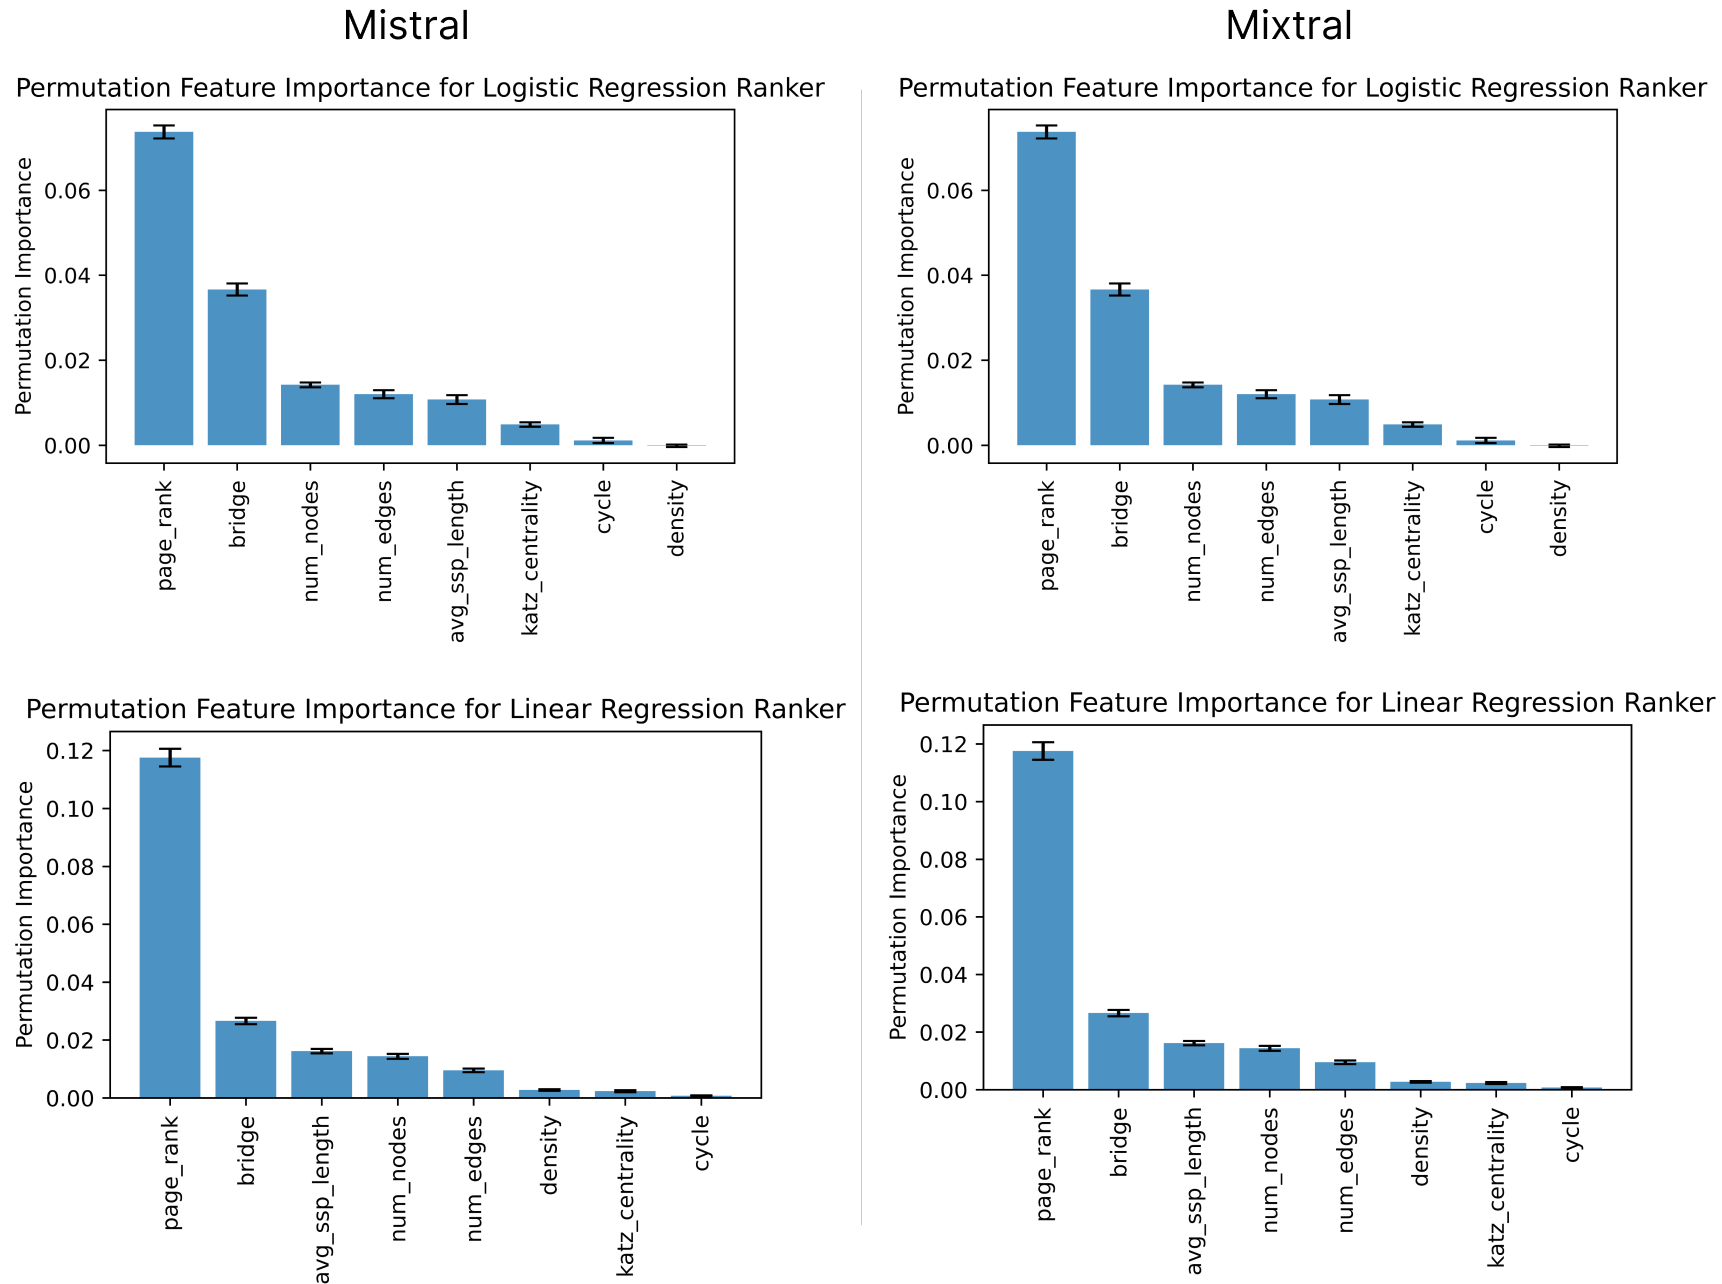
\includegraphics[width=\textwidth]{kg_path_fusion/feature_importance_mistral_mixtral.png}
   \caption{Permutation importance of graph features for Linear and Logistic Regression rankers on answer candidates generated by Mistral and Mixtral. The results show how different features contribute to the ranking performance for these state-of-the-art models.}
   \label{fig:controllable_fusion:feature_importance_mistral_mixtral}
\end{figure}

Lastly, we conducted a comprehensive analysis of feature importance for our gradient-boosting rankers, specifically focusing on the CatBoost implementation. This analysis is particularly interesting because CatBoost offers unique capabilities in handling diverse feature types. Unlike traditional regression-based rankers, CatBoost natively supports a wide range of feature formats:

\begin{enumerate}
    \item Numerical features, which represent continuous values
    \item Categorical features, which represent discrete categories
    \item Text features, which contain natural language content
    \item Embedding features, which capture semantic information in vector form
\end{enumerate}

This versatility in feature handling is particularly advantageous for our task, as it allows us to process embedding features without the need to split them into individual components, unlike the regression-based approaches discussed earlier. This capability makes it possible to assess the importance of both graph-based features and embedding-like features simultaneously, providing a more holistic view of feature contributions.

However, we encountered a limitation in CatBoost's native embedding support. The framework uses order target encodings for embedding features, which introduces ambiguity in the interpretation of results. Additionally, this embedding algorithm is not widely adopted in the natural language processing community, making it less suitable for our specific use case. Given our focus on end-user requirements and practical applicability, we decided to exclude this component from our analysis.

The results of our feature importance analysis for CatBoost rankers are presented in two figures: Figure~\ref{fig:controllable_fusion:feature_importance_t5_large_xl_catboost} shows the analysis for T5-Large-SSM and T5-XL-SSM models, while Figure~\ref{fig:controllable_fusion:feature_importance_mis_mix_catboost} presents the results for Mistral and Mixtral models.

\begin{figure}[htb]
   \centering
   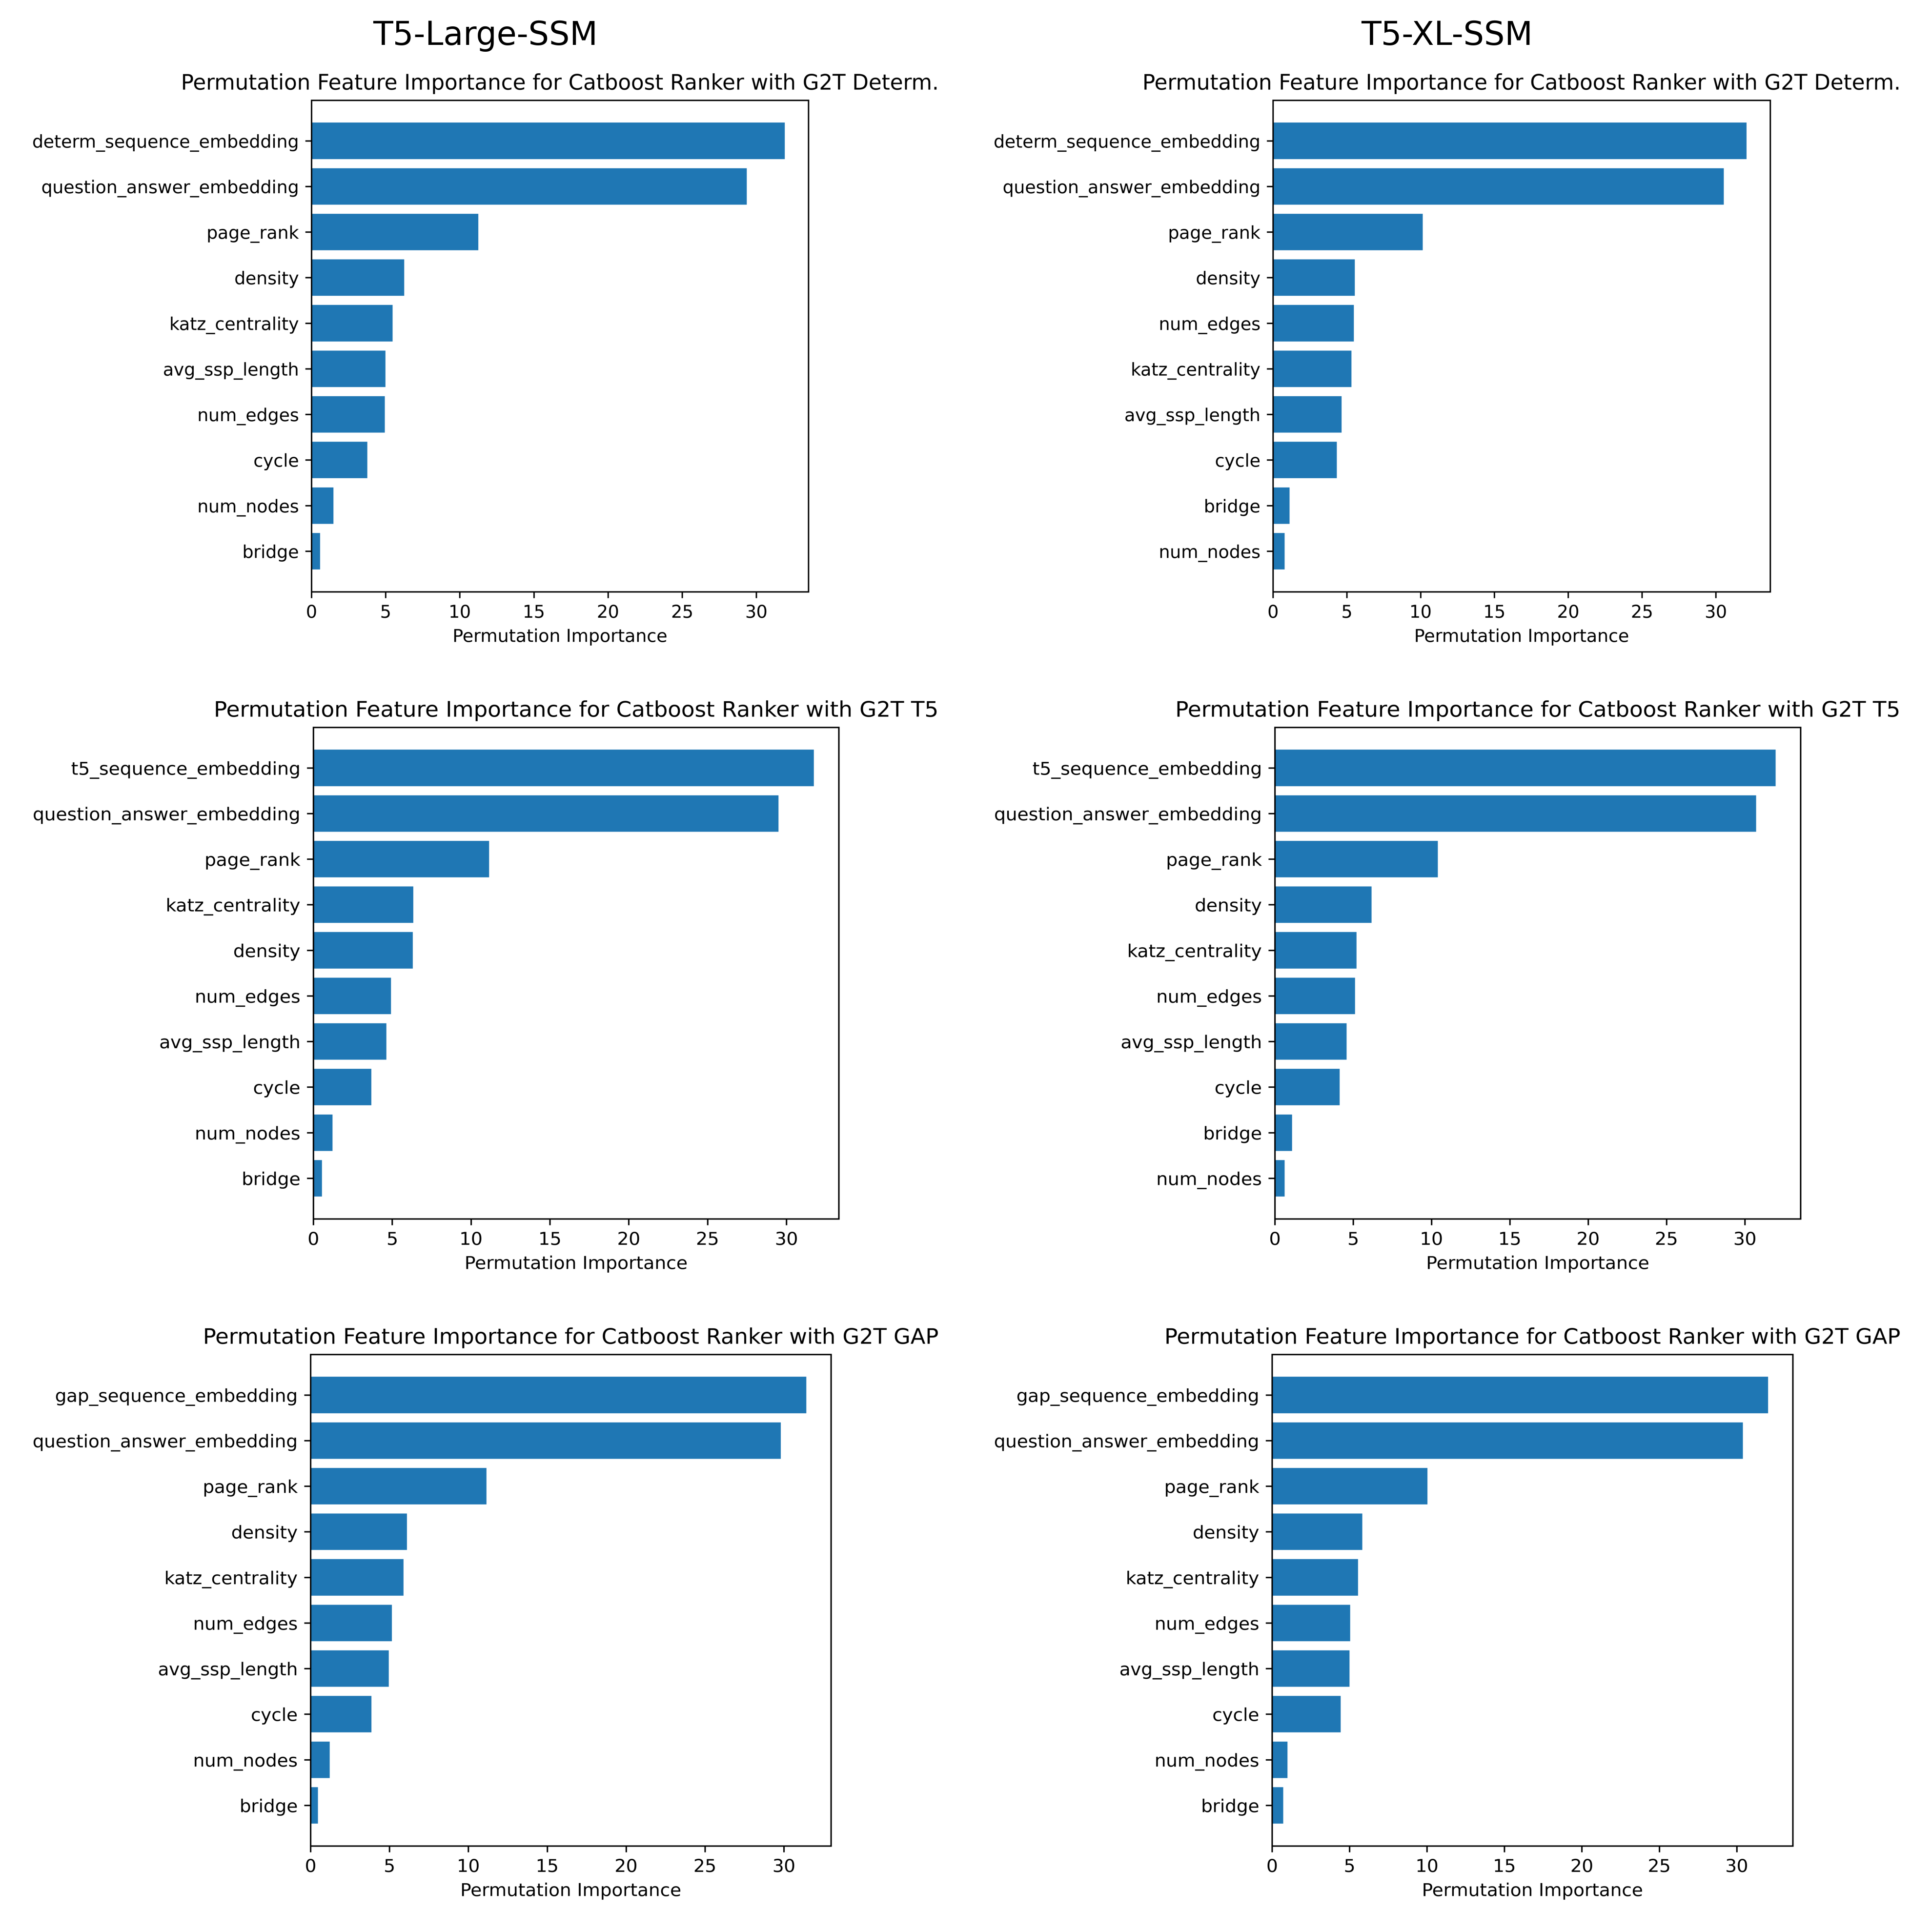
\includegraphics[width=\textwidth]{kg_path_fusion/t5xl_large_catboost.png}
   \caption{Permutation importance of graph, text, and Graph2Text features for CatBoost rankers on answer candidates generated by T5-Large-SSM and T5-XL-SSM. The analysis reveals the relative contribution of different feature types to the model's performance.}
   \label{fig:controllable_fusion:feature_importance_t5_large_xl_catboost}
\end{figure}

\begin{figure}[htb]
   \centering
   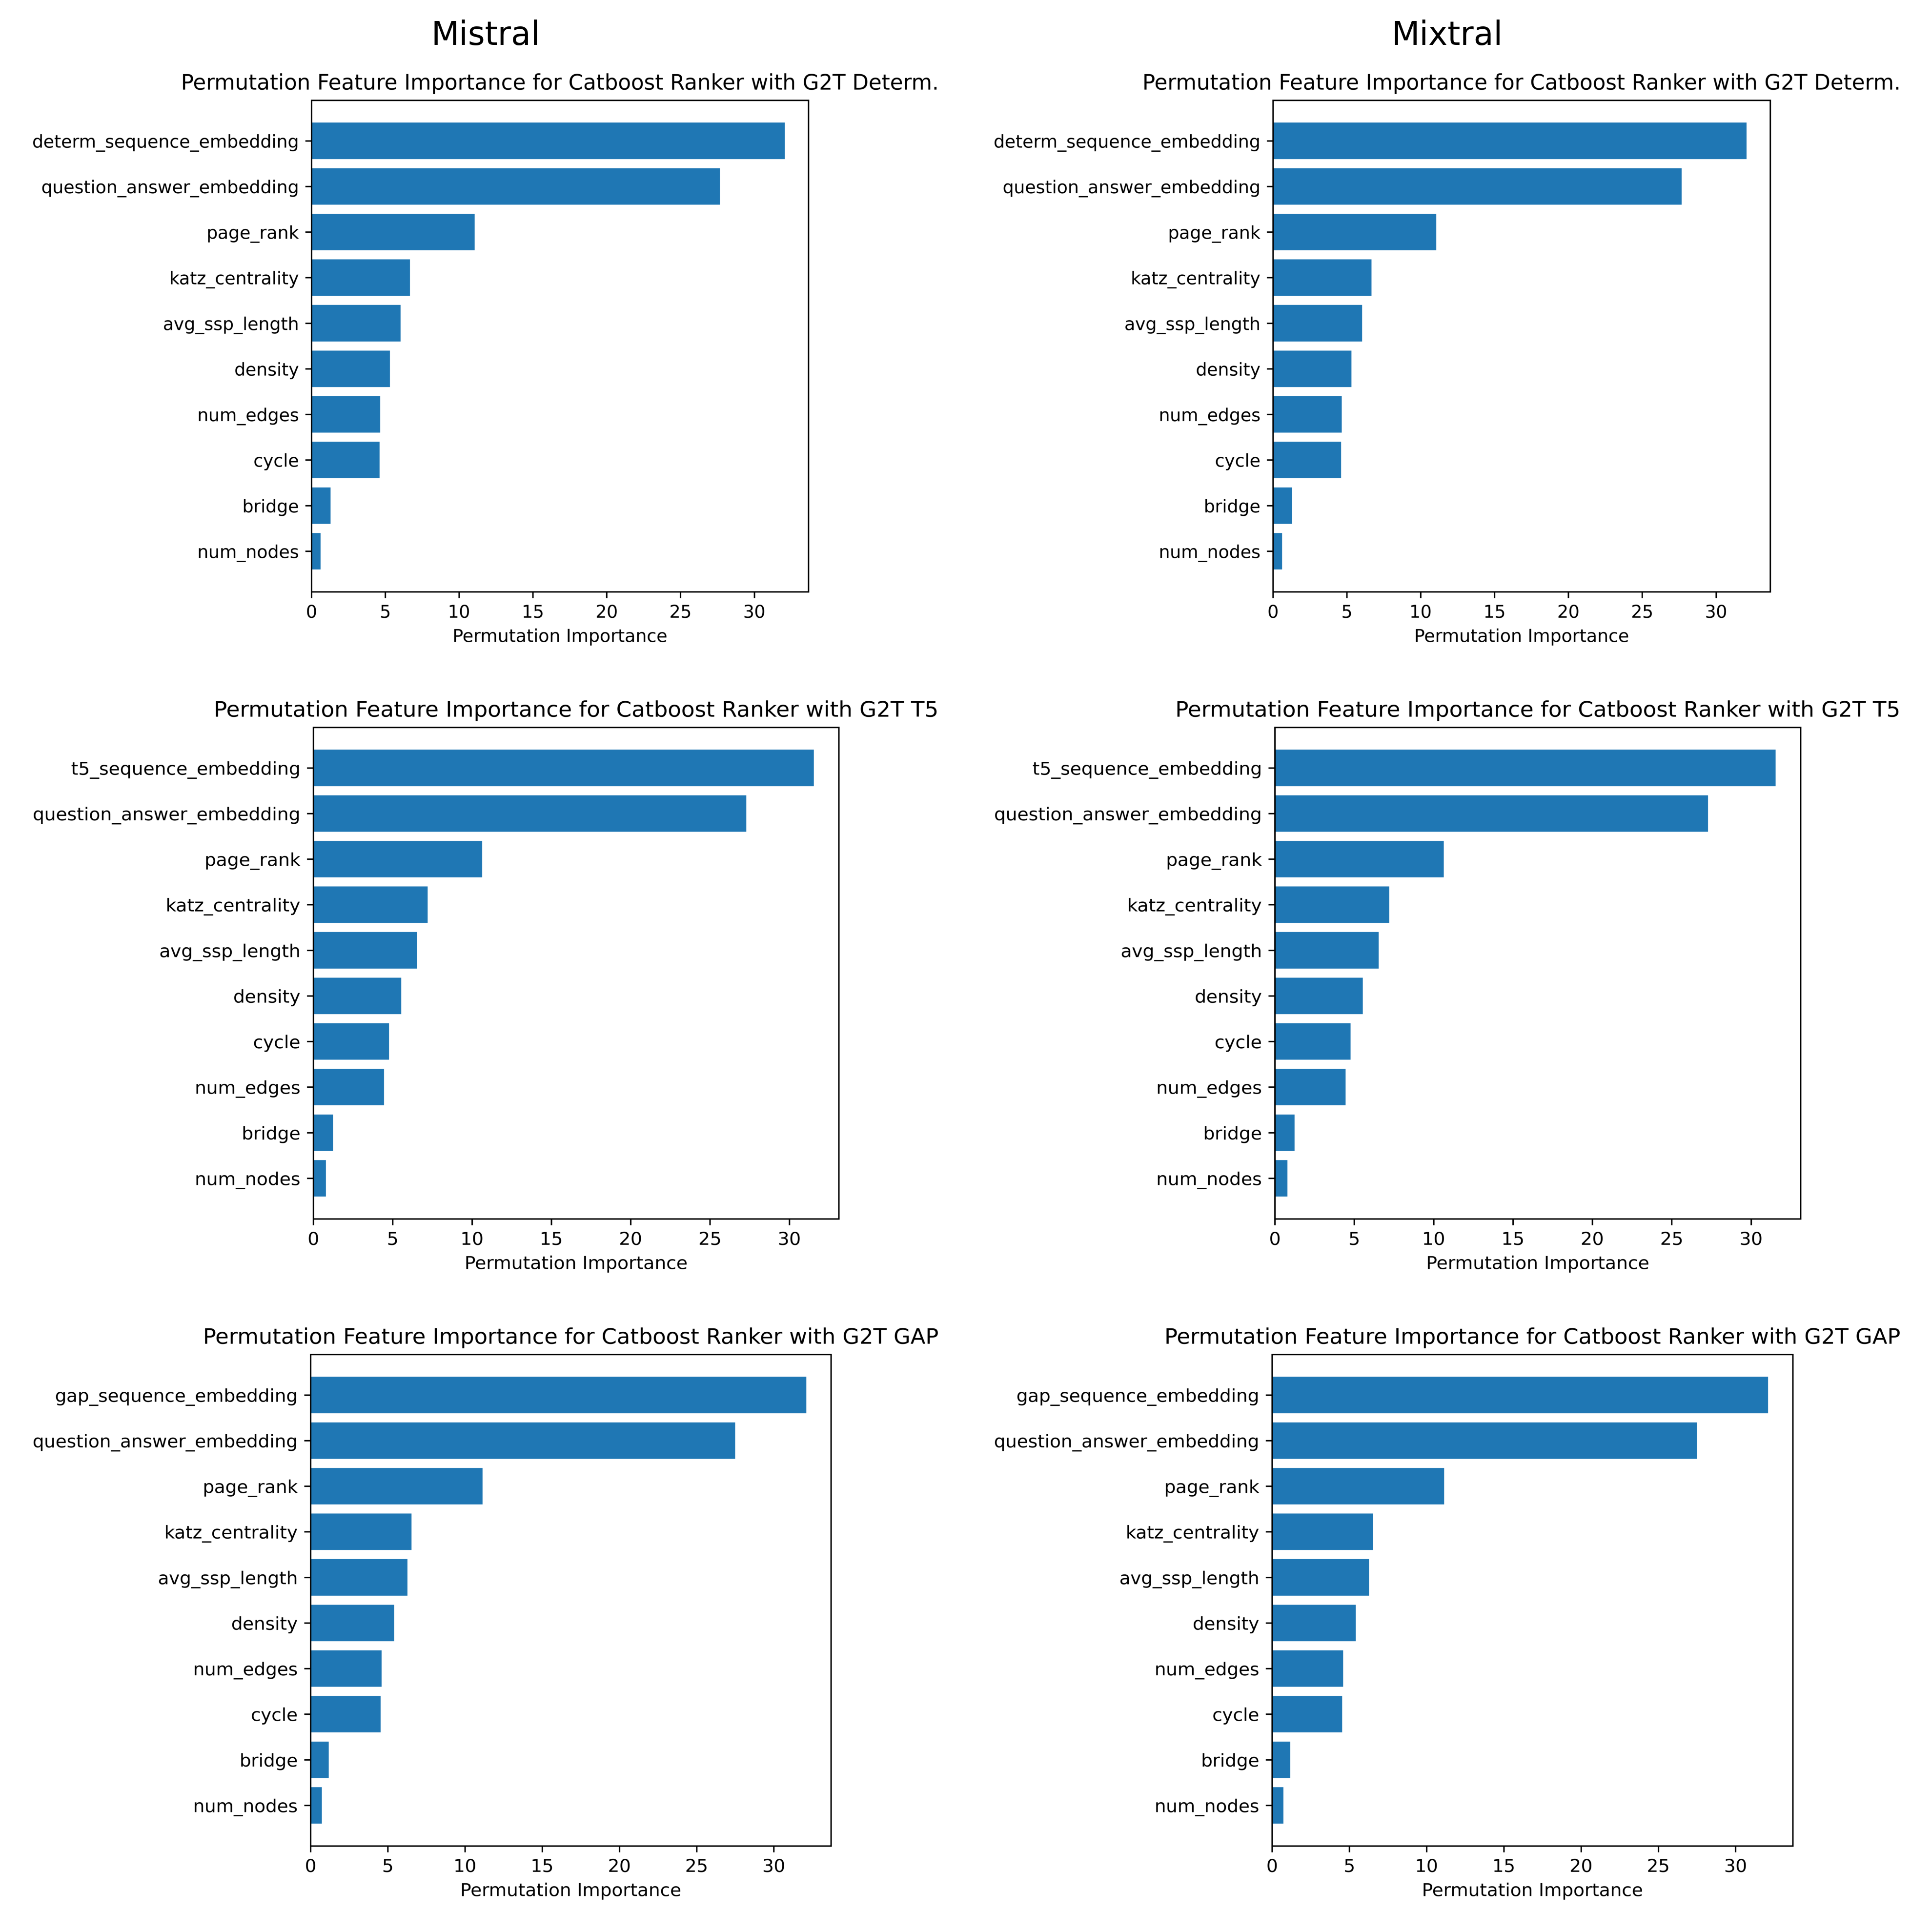
\includegraphics[width=\textwidth]{kg_path_fusion/mistral_mixtral_catboost.png}
   \caption{Permutation importance of graph, text, and Graph2Text features for CatBoost rankers on answer candidates generated by Mistral and Mixtral. The results demonstrate how different feature types contribute to the ranking performance for these state-of-the-art models.}
   \label{fig:controllable_fusion:feature_importance_mis_mix_catboost}
\end{figure}

A detailed examination of the results reveals several significant patterns:

\begin{enumerate}
    \item \textbf{Dominance of Text Features}: The Graph2Text sequence and text features consistently demonstrate the highest importance across all models. This finding strongly supports our earlier observations about the effectiveness of text-based features in the reranking process. The inclusion of initial questions in the feature set appears to be particularly crucial for the ranker's performance.
    
    \item \textbf{Graph Feature Importance}: Among the graph-based features, PageRank emerges as a consistently important factor for both T5-based models and the more recent Mistral/Mixtral models. This observation reinforces the value of PageRank in both classical graph classification tasks and Knowledge Graph Question Answering (KGQA) applications. Other notable graph features include:
    \begin{itemize}
        \item Graph density, which measures the connectivity of the subgraph
        \item Katz centrality, which captures the influence of nodes in the graph
        \item Average shortest path length between question entities and answer candidates
    \end{itemize}
    
    \item \textbf{Model-Specific Variations}: The importance of features varies between different model types, with some features showing higher importance for T5-based models compared to Mistral/Mixtral, and vice versa. This variation suggests that different language models may benefit from different feature combinations.
\end{enumerate}

These findings have important implications for the design of future reranking systems. The strong performance of text-based features suggests that they should be a core component of any reranking system, while the varying importance of graph features across different models indicates that feature selection should be tailored to the specific characteristics of the underlying language model.

\subsection{Hits@N Evaluation Results}

While Hits@1 provides a valuable metric for assessing the top-ranked answer, it offers only a partial view of the reranking approaches' effectiveness. As discussed in Section~\ref{sec:controllable_fusion:evaluation}, we employ the Hits@N metric to conduct a comprehensive analysis of all rankers and feature sets. This broader evaluation allows us to understand how the reranking process affects the entire sequence of candidate answers, not just the top prediction.

In this subsection, we present a detailed analysis of answer sequences both before and after reranking. Our evaluation encompasses:

\begin{enumerate}
    \item \textbf{Comprehensive Testing}: All proposed methods have been evaluated across different feature combinations and model configurations to ensure robust results.
    
    \item \textbf{Multiple N Values}: We calculate Hits@N for various values of N (specifically N=1, 2, and 3) to capture the performance improvements at the top of the ranked list. This approach helps us understand:
    \begin{itemize}
        \item How quickly the correct answer appears in the ranked list
        \item The distribution of correct answers across different positions
        \item The overall effectiveness of the reranking process
    \end{itemize}
    
    \item \textbf{Model Comparisons}: We analyze the performance of different reranking approaches, including:
    \begin{itemize}
        \item Initial predictions from the base language models
        \item Baseline reranking methods
        \item Our proposed approaches with various feature combinations
    \end{itemize}
\end{enumerate}

The detailed results for all combinations of answer candidate sources (T5-Large-SSM, T5-XL-SSM, Mistral, and Mixtral), reranking models, and feature sets are presented in Tables~\ref{tab:controllable_fusion:t5_large_ssm_all_results}, \ref{tab:controllable_fusion:t5_xl_ssm_all_results}, \ref{tab:controllable_fusion:mistral_all_results}, and~\ref{tab:controllable_fusion:mixtral_all_results}. These tables provide a granular view of the Hits@1, Hits@2, and Hits@3 scores, demonstrating the potential of utilizing subgraphs to rerank LLM responses. Moreover, these results underscore the importance of accurately transferring all relevant information from the subgraph to the reranking model. Consequently, the outcomes of this process significantly depend on the quality of the Graph2Text process.

Figure~\ref{fig:controllable_fusion:hit_at_n_plot_all} presents a visual summary of the most significant findings from our comprehensive evaluation, illustrating the overall trends. The results demonstrate several key patterns:

\begin{enumerate}
    \item \textbf{MPNet Superiority}: The reranking approach using MPNet with text and Graph2Text features consistently outperforms both the initial predictions and baseline models. This improvement is particularly notable in the critical Hits@1 metric, where the correct answer appears as the top prediction more frequently.
    
    \item \textbf{Size-Independent Improvement}: The quality enhancement in Hits@1 answers is observed consistently across different language model sizes. This suggests that our reranking approach is robust and effective regardless of the underlying model's complexity.
    
    \item \textbf{Progressive Enhancement}: The improvements in performance are not limited to the top-ranked answer. The reranking process enhances the overall quality of the answer sequence, making it more likely for correct answers to appear in higher positions, as evidenced by the Hits@2 and Hits@3 scores.
\end{enumerate}

These findings underscore the effectiveness of our proposed reranking approach and highlight the importance of considering the entire answer sequence when evaluating question-answering systems. The consistent improvements across different model sizes and the enhanced quality of the top-ranked answers demonstrate the practical value of our methodology.

\begin{figure}[htbp]
   \centering
   \includegraphics[width=0.99\textwidth]{kg_path_fusion/hit_at_n_plot_all.pdf}
   \caption{Comparison of Hits@N performance across different reranking approaches on the Mintaka dataset. The plot shows the cumulative accuracy (Hits@N) for various values of N, demonstrating the effectiveness of different feature combinations and reranking models. The MPNet-based approach with text and Graph2Text features shows consistent improvement over baseline models and initial predictions, particularly in the critical Hits@1 metric. Results are shown for answers generated using Diverse Beam Search across different language model sizes.}
   \label{fig:controllable_fusion:hit_at_n_plot_all}
\end{figure}

\begin{table}[htbp]
    \caption{Hits@1-3 for all proposed reranking approaches and features after reranking the T5-Large-SSM generated answer candidates.}
    \label{tab:controllable_fusion:t5_large_ssm_all_results}
    \fontsize{9pt}{11pt}\selectfont
    \centering
    \setlength{\tabcolsep}{3pt}
    \begin{tabular}{l p{5cm} c c c}
        \toprule
        \textbf{Reranking Model} & \textbf{Features} & \textbf{Hits@1} & \textbf{Hit@2} & \textbf{Hit@3} \\
        \midrule
        Without reranking & & 0.2395 & 0.3580 & 0.4020 \\
        \cmidrule(lr){1-5}
        Full random & & 0.0278 & 0.0562 & 0.0828 \\
        \cmidrule(lr){1-5}
        Semantic reranking & Text & 0.0298 & 0.0647 & 0.0965 \\
        \cmidrule(lr){1-5}
        \multirow{9}{*}{Linear Regression} & Text & 0.2695 & 0.4502 & 0.5400 \\
        & Graph & 0.2338 & 0.4007 & 0.5000 \\
        & Text + Graph & 0.2953 & 0.4697 & 0.5558 \\
        & G2T (Det. Lin.) & 0.2550 & 0.4262 & 0.5230 \\
        & G2T (T5) & 0.2505 & 0.4230 & 0.5193 \\
        & G2T (GAP) & 0.2393 & 0.4133 & 0.5123 \\
        & Text + Graph + G2T (Det. Lin.) & \textbf{0.3065} & 0.4873 & 0.5755 \\
        & Text + Graph + G2T (T5) & 0.3070 & 0.4835 & 0.5710 \\
        & Text + Graph + G2T (GAP) & 0.3033 & 0.4870 & 0.5728 \\
        \midrule
        \multirow{12}{*}{Logistic Regression} & Text & 0.2605 & 0.4353 & 0.5360 \\
        & Graph & 0.2335 & 0.4040 & 0.4980 \\
        & Text + Graph & 0.2470 & 0.4240 & 0.5218 \\
        & G2T (Det. Lin.) & 0.2440 & 0.4203 & 0.5163 \\
        & G2T (T5) & 0.2313 & 0.4068 & 0.5028 \\
        & G2T (GAP) & 0.2925 & 0.4688 & 0.5625 \\
        & Text + Graph + G2T (Det. Lin.) & \textbf{0.3060} & 0.4873 & 0.5745 \\
        & Text + Graph + G2T (T5) & 0.2794 & 0.4780 & 0.5668 \\
        & Text + Graph + G2T (GAP) & 0.2925 & 0.4688 & 0.5625 \\
        \midrule
        \multirow{12}{*}{CatBoost} & Text & 0.2458 & 0.3753 & 0.4525 \\
        & Graph & 0.1935 & 0.3353 & 0.4238 \\
        & Text + Graph & 0.1975 & 0.3463 & 0.4510 \\
        & G2T (Det. Lin.) & 0.2405 & 0.4178 & 0.5068 \\
        & G2T (T5) & 0.2398 & 0.4025 & 0.4868 \\
        & G2T (GAP) & 0.2395 & 0.3975 & 0.4873 \\
        & Text + Graph + G2T (Det. Lin.) & 0.1808 & 0.3208 & 0.4120 \\
        & Text + Graph + G2T (T5) & 0.1888 & 0.3318 & 0.4233 \\
        & Text + Graph + G2T (GAP) & 0.1915 & 0.3350 & 0.4268 \\
        \midrule
        \multirow{10}{*}{MPNet} & Text & 0.2620 & 0.4380 & 0.5345 \\
        & Text + G2T (Det. Lin.) & 0.3399 & 0.5095 & 0.5900 \\
        & Text + G2T (Det. Lin.) + HL & 0.3105 & 0.4853 & 0.5735 \\
        & Text + G2T (T5) & \textbf{0.3493} & 0.5203 & 0.5945 \\
        & Text + G2T (T5) + HL & 0.3468 & 0.5178 & 0.5938 \\
        & Text + G2T (GAP) & 0.3395 & 0.5080 & 0.5890 \\
        & Text + G2T (GAP) + HL & 0.3435 & 0.5170 & 0.5973 \\
        \bottomrule
    \end{tabular}
\end{table}

\begin{table}[htbp]
    \setlength{\tabcolsep}{3pt}
    \caption{Hits@1-3 for all proposed reranking approaches and features after reranking the T5-XL-SSM generated answer candidates.}
    \label{tab:controllable_fusion:t5_xl_ssm_all_results}
    \fontsize{9pt}{11pt}\selectfont
    \centering
    \begin{tabular}{l p{5cm} c c c}
        \toprule
        \textbf{Reranking Model} & \textbf{Features} & \textbf{Hits@1} & \textbf{Hit@2} & \textbf{Hit@3} \\
        \midrule
        Without reranking & & 0.3042 & 0.4298 & 0.4688 \\
        \cmidrule(lr){1-5}
        Full random & & 0.0235 & 0.0473 & 0.0723 \\
        \cmidrule(lr){1-5}
        Semantic reranking & Text & 0.0245 & 0.0545 & 0.0830 \\
        \cmidrule(lr){1-5}
        \multirow{9}{*}{Linear Regression} & Text & 0.2955 & 0.4763 & 0.4763 \\
        & Graph & 0.2550 & 0.4353 & 0.5285 \\
        & Text + Graph & 0.3003 & 0.4825 & 0.5693 \\
        & G2T (Det. Lin.) & 0.2640 & 0.4480 & 0.5375 \\
        & G2T (T5) & 0.2593 & 0.4438 & 0.5333 \\
        & G2T (GAP) & 0.2563 & 0.4320 & 0.5215 \\
        & Text + Graph + G2T (Det. Lin.) & \textbf{0.3220} & 0.5073 & 0.5915 \\
        & Text + Graph + G2T (T5) & 0.3170 & 0.5035 & 0.5818 \\
        & Text + Graph + G2T (GAP) & 0.3153 & 0.5023 & 0.5793 \\
        \midrule
        \multirow{12}{*}{Logistic Regression} & Text & 0.2850 & 0.4683 & 0.5603 \\
        & Graph & 0.2613 & 0.4385 & 0.5283 \\
        & Text + Graph & 0.3003 & 0.4825 & 0.5693 \\
        & G2T (Det. Lin.) & 0.2598 & 0.4420 & 0.5423 \\
        & G2T (T5) & 0.2538 & 0.4393 & 0.5315 \\
        & G2T (GAP) & 0.2503 & 0.4310 & 0.5218 \\
        & Text + Graph + G2T (Det. Lin.) & \textbf{0.3210} & 0.5025 & 0.5885 \\
        & Text + Graph + G2T (T5) & 0.3080 & 0.4955 & 0.5778 \\
        & Text + Graph + G2T (GAP) & 0.3043 & 0.4908 & 0.5815 \\
        \midrule
        \multirow{12}{*}{CatBoost} & Text & 0.2593 & 0.3985 & 0.4720 \\
        & Graph & 0.2760 & 0.4573 & 0.5433 \\
        & Text + Graph & 0.1950 & 0.3370 & 0.4298 \\
        & G2T (Det. Lin.) & 0.2580 & 0.4218 & 0.5130 \\
        & G2T (T5) & 0.2485 & 0.4158 & 0.5025 \\
        & G2T (GAP) & 0.2590 & 0.4390 & 0.5258 \\
        & Text + Graph + G2T (Det. Lin.) & 0.1738 & 0.3160 & 0.4065 \\
        & Text + Graph + G2T (T5) & 0.1670 & 0.3168 & 0.4048 \\
        & Text + Graph + G2T (GAP) & 0.1660 & 0.3093 & 0.4048 \\
        \midrule
        \multirow{10}{*}{MPNet} & Text & 0.3418 & 0.5185 & 0.5960 \\
        & Text + G2T (Det. Lin.) & \textbf{0.3923} & 0.5648 & 0.6260 \\
        & Text + G2T (Det. Lin.) + HL & 0.3628 & 0.5453 & 0.6175 \\
        & Text + G2T (T5) & 0.3905 & 0.5610 & 0.6183 \\
        & Text + G2T (T5) + HL & 0.3760 & 0.5490 & 0.6160 \\
        & Text + G2T (GAP) & 0.3573 & 0.5315 & 0.6040 \\
        & Text + G2T (GAP) + HL & 0.3675 & 0.5528 & 0.6165 \\
        \bottomrule
    \end{tabular}
\end{table}

\begin{table}[htbp]
    \setlength{\tabcolsep}{3pt}
    \caption{Hits@1-3 for all proposed reranking approaches and features after reranking the Mistral generated answer candidates.}
    \label{tab:controllable_fusion:mistral_all_results}
    \fontsize{9pt}{11pt}\selectfont
    \centering
    \begin{tabular}{l p{5cm} c c c}
        \toprule
        \textbf{Reranking Model} & \textbf{Features} & \textbf{Hits@1} & \textbf{Hit@2} & \textbf{Hit@3} \\
        \midrule
        Without reranking & & 0.4655 & 0.5313 & 0.5590 \\
        \cmidrule(lr){1-5}
        Full random & & 0.0920 & 0.1585 & 0.2165 \\
        \cmidrule(lr){1-5}
        Semantic reranking & Text & 0.0858 & 0.1393 & 0.1790 \\
        \cmidrule(lr){1-5}
        \multirow{9}{*}{Linear Regression} & Text & 0.4760 & 0.5818 & 0.6173 \\
        & Graph & 0.3575 & 0.4918 & 0.5653 \\
        & Text + Graph & 0.4810 & 0.5848 & 0.6193 \\
        & G2T (Det. Lin.) & 0.3960 & 0.5298 & 0.5898 \\
        & G2T (T5) & 0.4013 & 0.5295 & 0.5910 \\
        & G2T (GAP) & 0.3885 & 0.5220 & 0.5845 \\
        & Text + G2T (Det. Lin.) & 0.4860 & 0.5875 & 0.6198 \\
        & Text + G2T (T5) & 0.4825 & 0.5845 & 0.6200 \\
        & Text + G2T (GAP) & 0.4770 & 0.5798 & 0.6180 \\
        \midrule
        \multirow{12}{*}{Logistic Regression} & Text & 0.4730 & 0.5795 & 0.6148 \\
        & Graph & 0.3558 & 0.4925 & 0.5645 \\
        & Text + Graph & 0.4745 & 0.5833 & 0.6200 \\
        & G2T (Det. Lin.) & 0.3970 & 0.5260 & 0.5960 \\
        & G2T (T5) & 0.3985 & 0.5305 & 0.5933 \\
        & G2T (GAP) & 0.3850 & 0.5195 & 0.5878 \\
        & Text + G2T (Det. Lin.) & 0.4790 & 0.5833 & 0.6210 \\
        & Text + G2T (T5) & 0.4745 & 0.5838 & 0.6205 \\
        & Text + G2T (GAP) & 0.4728 & 0.5785 & 0.6183 \\
        \midrule
        \multirow{12}{*}{CatBoost} & Text & 0.3918 & 0.5070 & 0.5708 \\
        & Graph & 0.3633 & 0.4995 & 0.5715 \\
        & Text + Graph & 0.3128 & 0.4443 & 0.5295 \\
        & G2T (Det. Lin.) & 0.3863 & 0.5078 & 0.5770 \\
        & G2T (T5) & 0.4013 & 0.5295 & 0.5910 \\
        & G2T (GAP) & 0.3788 & 0.5098 & 0.5775 \\
        & Text + G2T (Det. Lin.) & 0.2883 & 0.4208 & 0.5163 \\
        & Text + G2T (T5) & 0.2568 & 0.3843 & 0.4958 \\
        & Text + G2T (GAP) & 0.3013 & 0.4393 & 0.5265 \\
        \midrule
        \multirow{10}{*}{MPNet} & Text & 0.5115 & 0.6035 & 0.6273 \\
        & Text + G2T (Det. Lin.) & 0.5008 & 0.5913 & 0.6225 \\
        & Text + G2T (Det. Lin.) + HL & 0.5140 & 0.6013 & 0.6288 \\
        & Text + G2T (T5) & 0.4965 & 0.5913 & 0.6230 \\
        & Text + G2T (T5) + HL & 0.5148 & 0.6003 & 0.6253 \\
        & Text + G2T (GAP) & 0.4918 & 0.5880 & 0.6205 \\
        & Text + G2T (GAP) + HL & 0.5073 & 0.5988 & 0.6250 \\
        \bottomrule
    \end{tabular}
\end{table}

\begin{table}[htbp]
    \setlength{\tabcolsep}{3pt}
    \caption{Hits@1-3 for all proposed reranking approaches and features after reranking the Mixtral generated answer candidates.}
    \label{tab:controllable_fusion:mixtral_all_results}
    \fontsize{9pt}{11pt}\selectfont
    \centering
    \begin{tabular}{l p{5cm} c c c}
        \toprule
        \textbf{Reranking Model} & \textbf{Features} & \textbf{Hits@1} & \textbf{Hit@2} & \textbf{Hit@3} \\
        \midrule
        Without reranking & & 0.5173 & 0.5628 & 0.5735 \\
        \cmidrule(lr){1-5}
        Full random & & 0.0580 & 0.1090 & 0.1455 \\
        \cmidrule(lr){1-5}
        Semantic re-anking & Text & 0.0303 & 0.0550 & 0.0715 \\
        \cmidrule(lr){1-5}
        \multirow{9}{*}{Linear Regression} & Text & 0.4883 & 0.5883 & 0.6188 \\
        & Graph & 0.3698 & 0.4983 & 0.5668 \\
        & Text + Graph & 0.4933 & 0.5913 & 0.6208 \\
        & G2T (Det. Lin.) & 0.4083 & 0.5363 & 0.5913 \\
        & G2T (T5) & 0.4135 & 0.5360 & 0.5925 \\
        & G2T (GAP) & 0.4008 & 0.5285 & 0.5860 \\
        & Text + G2T (Det. Lin.) & 0.4983 & 0.5940 & 0.6213 \\
        & Text + G2T (T5) & 0.4948 & 0.5910 & 0.6215 \\
        & Text + G2T (GAP) & 0.4850 & 0.5850 & 0.6198 \\
        \midrule
        \multirow{12}{*}{Logistic Regression} & Text & 0.4853 & 0.5860 & 0.6163 \\
        & Graph & 0.3680 & 0.4990 & 0.5660 \\
        & Text + Graph & 0.4868 & 0.5898 & 0.6215 \\
        & G2T (Det. Lin.) & 0.4093 & 0.5325 & 0.5975 \\
        & G2T (T5) & 0.4108 & 0.5370 & 0.5948 \\
        & G2T (GAP) & 0.3973 & 0.5260 & 0.5893 \\
        & Text + G2T (Det. Lin.) & 0.4913 & 0.5898 & 0.6225 \\
        & Text + G2T (T5) & 0.4868 & 0.5903 & 0.6220 \\
        & Text + G2T (GAP) & 0.4850 & 0.5850 & 0.6198 \\
        \midrule
        \multirow{12}{*}{CatBoost} & Text & 0.4040 & 0.5135 & 0.5723 \\
        & Graph & 0.3755 & 0.5060 & 0.5730 \\
        & Text + Graph & 0.3250 & 0.4508 & 0.5310 \\
        & G2T (Det. Lin.) & 0.3985 & 0.5143 & 0.5785 \\
        & G2T (T5) & 0.3940 & 0.5143 & 0.5793 \\
        & G2T (GAP) & 0.3910 & 0.5163 & 0.5790 \\
        & Text + G2T (Det. Lin.) & 0.3005 & 0.4273 & 0.5178 \\
        & Text + G2T (T5) & 0.2690 & 0.3908 & 0.4973 \\
        & Text + G2T (GAP) & 0.3135 & 0.4458 & 0.5280 \\
        \midrule
        \multirow{10}{*}{MPNet} & Text & 0.5238 & 0.6100 & 0.6288 \\
        & Text + G2T (Det. Lin.) & 0.5130 & 0.5978 & 0.6240 \\
        & Text + G2T (Det. Lin.) + HL & 0.5263 & 0.6078 & 0.6303 \\
        & Text + G2T (T5) & 0.5088 & 0.5978 & 0.6245 \\
        & Text + G2T (T5) + HL & 0.5270 & 0.6068 & 0.6268 \\
        & Text + G2T (GAP) & 0.5040 & 0.5945 & 0.6220 \\
        & Text + G2T (GAP) + HL & 0.5195 & 0.6053 & 0.6265 \\
        \bottomrule
    \end{tabular}
\end{table}

The results highlight that combinations involving textual representations of subgraphs (Graph2Text sequences) and direct text features, especially when processed by neural rankers like MPNet, are particularly effective. For instance, the MPNet model leveraging ``Text + G2T (T5)'' or ``Text + G2T (Det. Lin.)'' features frequently achieves top performance. Furthermore, even simpler regression-based models show notable gains when provided with richer feature sets combining text, graph, and Graph2Text information, often surpassing the initial LLM performance. This underscores the value of integrating structured knowledge from KGs into the reranking pipeline, leading to more accurate and reliable answer selection in question-answering systems. The consistent uplift in performance, irrespective of the base LLM's scale, further reinforces the general applicability and benefit of these subgraph-based reranking techniques.

\section{ShortPathQA: Dataset for Controllable Fusion Knowledge Graphs and Large Language Models}
\label{sec:controllable_fusion:dataset}

Evaluating the effectiveness of methods that fuse Large Language Models (LLMs) with Knowledge Graph (KG) structures, like the subgraph-based reranking approaches discussed in this chapter, requires specific evaluation resources. While many Knowledge Graph Question Answering (KGQA) datasets exist (see Section~\ref{sec:rw_kgqa} for overview), they often focus on the end-to-end task, involving multiple complex stages like entity linking, relation extraction, and subgraph retrieval from massive KGs. This multi-stage nature makes it difficult to isolate and evaluate the performance of the fusion or reranking component itself, as errors can propagate from earlier stages. Furthermore, variations in how different systems extract subgraphs make direct comparison of subgraph processing or reranking techniques challenging~\cite{DBLP:conf/nldb/SalnikovSPQA25}.

Working directly with large-scale KGs like Wikidata also presents significant engineering challenges for many researchers. Tasks such as accurate entity linking, efficient shortest path calculation over billions of triples, and simply hosting the KG (Wikidata, for example, can require terabytes of RAM for efficient in-memory processing) demand substantial computational resources and specialized expertise. This overhead can divert focus from the core research question of how to best utilize the structural information within a KG once it is identified.

These challenges highlighted the need for a standardized dataset specifically designed to facilitate research on controllable fusion methods. Such a dataset should provide pre-computed, relevant KG subgraphs alongside questions and answer candidates, removing the burden of KG hosting and subgraph retrieval. This allows researchers to concentrate directly on developing and comparing models that reason over or rerank based on the provided graph structures. This motivated us to create and publish the ShortPathQA dataset~\cite{DBLP:conf/nldb/SalnikovSPQA25}, which we describe in the following subsections.

ShortPathQA is the first QA dataset that combines textual questions paired with pre-computed Wikidata KG subgraphs applying a unified yet simple subgraph construction approach. The overview of our dataset creation methodology is presented in Figure~\ref{fig:controllable_fusion:big_pipe}. Overall, three key steps should be highlighted: (1) answer candidate generation using an LM; (2) entity linking for both entities mentioned in a question as well as answer candidates from step (1); (3) KG subgraph retrieval with a unified shortest path methodology applied to all questions within a given questions collection.

The code for this dataset is available at \url{https://github.com/s-nlp/ShortPathQA}.

\subsection{Collection of Questions}\label{subsec:question_collection}

ShortPathQA dataset consists of 2 main parts: 
\begin{itemize}
    \item \textbf{Automatic:} A large collection of questions adopted from Mintaka corpus~\cite{DBLP:conf/coling/SenAS22-mintaka} 
    \item \textbf{Manual:} A small collection of new manually curated questions for detailed testing and analysis. 
\end{itemize}

ShortPathQA dataset in build on the Mintaka~\cite{DBLP:conf/coling/SenAS22-mintaka} question format, where each question is annotated with Wikidata entities mentioned in it. While Mintaka does not guarantee a correct answer to be a Wikidata entities, we a sample a subset of questions whose correct answers are the Wikidata entities. Specifically, we remove all \textit{count} questions based on question types provided in the dataset. 
% We refer to the filtered question subset  of our dataset build upon Mintaka questions as \textit{ShortPathQA}.  
% For questions inherited from Mintaka, we preserve the original train/test split (9,750 and 2,430 questions respectively). We will refer to these subsets as \textit{train set} and \textit{automatic test set}, respectively.

In addition to questions adopted from Mintaka, we release \textit{ShortPathQA Manual test set}, a collection of 350 new questions. For consistency with first part of dataset, each question is formulated based on a reference template question from the original Mintaka.  For instance, given a question \textit{``Who is older, The Weeknd or Drake?''} with answer \textit{Drake (Q33240)}, we construct a novel question \textit{``Who was born earlier, Nikolai Ushin or Yossi Abulafia?''} whose answer is \textit{``Nikolai Ushin (Q20203178)''}. 
For each new question, we ensure that it mentions at least one entity with a valid Wikidata identifier;and one or more correct answers to the new question are Wikidata entities. Both types of entities are linked to Wikidata manually.

For \textit{ShortPathQA Manual} test set,  we manually assess the quality of each new created question by ranking it on a scale from 1 to 5, where 1 is ``the given answer is completely irrelevant for the question'', 5 --- ``the given answer is comprehensive for  the given question''. Moreover, we label each question to the question type according to Mintaka classes. Each question was assigned with two annotators. The Kohen's kappa which represents the annotation agreement is $0.81$ for question type and $0.51$ for question quality, the average quality of the questions is $4.81$.


For each answer candidate $c \in \mathcal{A}_q \cup \mathcal{N}_q$, either correct or incorrect, we present the shortest path Wikidata subgraph $\mathcal{G}(q, c)$ describing the shortest path from each entity from $\mathcal{E}_q$ (mentioned in a question) to candidate entity $c$. A visual representation of this process is provided in Figure~\ref{fig:controllable_fusion:big_pipe}. Candidates generated by language model and linked to entities by Wikimedia provided search API\footnote{\href{https://www.mediawiki.org/wiki/Wikibase/API}{www.mediawiki.org/wiki/Wikibase/API}}. This process was detailed describe in Section~\ref{sec:controllable_fusion:answer_candidate_generation} and Section~\ref{sec:controllable_fusion:subgraph_extract}.


\subsection{Dataset Statistics}

Detailed statistics of the proposed ShortPathQA dataset is summarized in Table~\ref{tab:data_statistics}. As seen from the table, our dataset provides over 143K question-candidate pairs with relevant KG subgraphs covering over 32K unique concepts from the Wikidata KG. Notably, the number of Wikidata nodes being answer candidates (26.1K) is higher then the unique candidate name count (24.7K). This implies that some answer candidates can be indistinguishable between each other from their textual names only and relevant KG subgraphs might help overcome the ambiguity.

\begin{table*}[t!]
\centering
\caption{Detailed statistics of the ShortPathQA dataset, including the number of questions, answers, candidates, Wikidata entities mentioned in questions and answer candidates, as well as shortest path graph sizes. \textbf{Test (A)} and \textbf{Test (M)} stand for automatic and manual test sets, respectively.}
\label{tab:data_statistics}
\resizebox{\textwidth}{!}{
    \begin{tabular}{l|cccc||l|cccc}
        \toprule
        % & \multicolumn{4}{c}{\textbf{Subset}} & &\multicolumn{4}{c}{\textbf{Candidate graphs statistics}}  \\
        \multicolumn{5}{c||}{\textbf{Question \& candidate statistics}} & \multicolumn{5}{c}{\textbf{Candidate graphs statistics}}  \\
        \cmidrule{1-5} \cmidrule{6-10}
        \textbf{Statistics} & \textbf{Train} & \textbf{Test (A)} & \textbf{Test (M)} & \textbf{Total} & \textbf{Statistics} & \textbf{Train} & \textbf{Test (A)} & \textbf{Test (M)} & \textbf{Total} \\ \midrule
        \textbf{Questions} & 9,750 & 2,430 & 350 & 12,526 & \textbf{Nodes} & 371,372 & 46,757 & 17,058 & 435,187 \\
        % \multicolumn{5}{c}{\textbf{Answer candidates}} \\
        % \midrule
        \textbf{Candidates} & 123,666 & 15,577 & 3,818 & 143,061 & \textbf{Unique nodes} & 25,457 & 9,867 & 4,895 & 32,226 \\
        % \textbf{Candidate names} & 19,956 & 7,789 & 2,979 & 24,773 \\
        \textbf{Unique names} & 19,956 & 7,789 & 2,979 & 24,773 & \textbf{Avg. \# nodes} & 3 & 3 & 4.47 & 3.04  \\
        % \cmidrule{1-5}\cmidrule{6-10}
        \multicolumn{5}{c||}{\textbf{Covered Wikidata nodes}} & \textbf{Edges} & 423,552 & 53,461 & 21,557 &  498,570  \\
        % \cmidrule{1-5}
        \textbf{Mentioned} & 4,456 & 1,679 & 497 & 5,401 & \textbf{Edge types} & 593 & 450 & 318 & 635 \\
        \textbf{Candidate} & 20,856 & 8,025 & 3,278 & 26,169 & \textbf{Avg. \# edges} & 3.42 & 3.43 & 5.65 & 3.49  \\
        \bottomrule
    \end{tabular}
}
\end{table*}

\subsection{Baseline Evaluation}

To motivate usage of our dataset, we evaluate the performance of the different KGQA approaches on our dataset: (i) zero-shot LLM prediction; (ii) supervised finetuning of LLMs, both an encoder-only Transformer~\cite{DBLP:conf/nips/VaswaniSPUJGKP17} and modern LLM decoder-only model LLaMA3-8b-Instruct~\cite{DBLP:journals/corr/abs-2407-21783-llama3}; (iii) positive/negative class constant; (iv) random baseline. For the first approach, we employ GPT4o, GPT4o mini, and LLaMA3-8b-Instruct models and experiment with adding graph information to the prompt. For the second approach, we adopt the graph linearization approach of~\cite{DBLP:journals/corr/abs-2310-02166} to create a textual representation of an input graph with candidate answers highlighted by special separator tokens. We present both of them in the subsections below.

\subsubsection{Supervised Fine-tuning}
As supervised fine-tuning, we adopt MPNet\footnote{\href{https://huggingface.co/sentence-transformers/all-mpnet-base-v2}{huggingface:sentence-transformers/all-mpnet-base-v2}}~\cite{DBLP:conf/nips/Song0QLL20} and LLaMA3-8B-Instruct~\cite{DBLP:journals/corr/abs-2407-21783-llama3} to encode both questions and linearized subgraphs. The task is formulated as a binary classification: given a question $q$, answer candidate $c$, and KG subgraph $\mathcal{G}(q, c)$, a model has to identify $c$ is a correct answer for $q$. 
We experiment with two input types: (i) \textbf{No Graph}: a model is passed with textual information only: $q\,[SEP]\,c$; (ii) \textbf{With Graph}: a model can reason over graph $\mathcal{L}(q, c)$ to answer observed question: $q\, [SEP] \mathcal{L}(q, c)$. The linearization $\mathcal{L}(q, c)$ of graph $\mathcal{G}(q, c)$ is obtained iteratively by traversing and linearizing individual edges while moving from the mentioned entities $\mathcal{E}_q$ to the answer candidate $c$. 
Each edge $(h, r, t)$ is linearized as $"h, r, t"$. If either $h=c$ or $t=c$, they are additionally emphasized with separator tokens  ``[SEP]'' for the MPNet model: e.g., ``$[SEP]\,h\,[SEP],\,r,\,t$'' if $h=c$. 

For supervised baselines, we use 10\% random questions as validation set for tuning hyper-parameters.
We train each supervised for 10 epochs with a batch size of 32 and learning rate of 1e-5 using Adam optimizer~\cite{DBLP:journals/corr/KingmaB14}. For prediction, we load the model weights from the best epoch in terms of validation F1-score.

The LLaMA3-8B-Instruct model was fine-tuned in a chat format that accepts system messages with short instructions and user messages with questions, answers, and, for the version that accepts subgraphs, a graph in linearized format without tokens. It was trained on 1 epoch of the training dataset. 

\subsubsection{Zero-shot Evaluation}

For zero-shot LLM-based baselines, we ask a model to select correct answers for a question $q$ from the given candidate list $C_q$. If multiple candidates have a matching textual name, we append edge types leading to each candidate $c$ in graph $\mathcal{G}(q, c)$. For example, for the question \textit{"Which film directed by James Cameron became the highest-grossing movie of all time?"} with two candidates answers named "Titanic": (i) \textit{1997 film by James Cameron} and (ii) \textit{1953 film by Jean Negulesco} the candidates are (i) \textit{Titanic (director)} and (ii) \textit{Titanic (original language of performance work)}, respectively. 

Prompt template for all models presented in Table~\ref{tab:controllable_fusion:shortpathqa:prompt_with_subgraph}. For \textbf{No KG} version, we did not used Graph part of user prompt, system prompt was simple instuction: \textit{You are a helpful assistant that verifies answers to questions.}. We employ the OpenAI LLMs\footnote{\href{https://chat.openai.com}{chat.openai.com}} (versions \textit{o3-mini}, \textit{GPT-4o} and \textit{GPT-4o mini}) and LLaMA3-8B-Instruct\footnote{\href{https://huggingface.co/meta-llama/Meta-Llama-3-8B-Instruct}{huggingface:meta-llama/Meta-Llama-3-8B-Instruct}}.

\begin{table*}[htb]
    \caption{LLM prompt to LLaMA3-8b-Instruct, o3-mini, GPT-4o and GPT-4o-mini when given additional subgraph information.}
    \label{tab:controllable_fusion:shortpathqa:prompt_with_subgraph}
        \centering
        \resizebox{\textwidth}{!}{
        \begin{tabular}{>{\raggedright\arraybackslash}p{0.99\textwidth}}
            \toprule
            \makecell[c]{\textbf{System}} \\ \hline
            You are an AI assistant tasked with evaluating the correctness of answers to questions based on 
            provided graph information. The graph consists of triplets in the format (subject, property, 
            object) that demonstrate the shortest path between the question entity and the answer entity.
            \par
            Your role is to:
            \par
              1. Analyze the question and the provided answer carefully.\par
              2. Examine the graph triplets to find connections between the question entity and the answer
                 entity.\par
              3. Evaluate if the shortest path in the graph supports the given answer.\par
              4. Consider that some paths may appear unrelated to the question at first glance but could 
                 still lead to the correct answer.\par
              5. Conclude whether the answer is correct, partially correct, or incorrect based on the graph
                 information.\par
              6. If the answer is incorrect or partially correct, suggest the correct answer based on the 
                 graph data.\par
              7. Provide a short answer.
            \par
            Remember to be thorough in your analysis and clearly communicate your thought process. Your goal 
            is to provide an accurate assessment of the answer's correctness while considering all relevant 
            information from the graph. \\
            \hline
            \makecell[c]{\textbf{User}} \\ \hline
            f"Question: \{q\}\par
            Graph: \{linearize\_graph(g, a, sep\_token=' ')\}\par
            Answer: \{a\} Is this answer correct? Respond with Yes or No:" \\
            \bottomrule
        \end{tabular}
        }
\end{table*}


\subsubsection{Experimental Results}

Evaluation results in terms of positive class precision, recall and F1-score are presented in Table~\ref{tab:controllable_fusion:shortpathqa:res_baselines}. Based on our experiments, GPT-4o is the best model for QA without using subgraphs.

\begin{table*}[ht!]
    \caption{Evaluation results on ShortPathQA test set. Precision, recall, and F1-score are calculated for positive class. o3-mini used with low reasoning effort. The best set-up for each backbone LM is highlighted with \textbf{bold}. The best overall F1-score for each test set is \underline{underlined}.}
    \label{tab:controllable_fusion:shortpathqa:res_baselines}
    \centering
    \resizebox{\textwidth}{!}{
    \begin{tabular}{lcccccc}
        \toprule
        
        \multirow{2}{*}{\textbf{Model setup}} & \multicolumn{3}{c}{\textbf{Automatic Test Set}} & \multicolumn{3}{c}{\textbf{Manual Test Set}} \\ \cmidrule{2-4} \cmidrule{5-7}
        
        & \textbf{Precision}  & \textbf{Recall} & \textbf{F1-score} & \textbf{Precision}  & \textbf{Recall} & \textbf{F1-score}   \\
        \midrule
        Negative class constant & 0.0 & 0.0 & 0.0 & 0.0 & 0.0 & 0.0 \\
        Positive class constant & 0.148 & 1.0 & 0.257 & 0.094 &  1.00 & 0.172 \\
        Random baseline & 0.148 & 0.5 & 0.228 & 0.094 &  0.5 & 0.158 \\
        \midrule
        \multicolumn{7}{c}{\textbf{Supervised evaluation}} \\
        
        
        \midrule
        MPNet (no KG)  & 0.503 & \textbf{0.639} & 0.563  &
        0.167 & 0.507 & 0.251  \\
        MPNet (with KG)  & \textbf{0.609} & 0.631 & \textbf{0.620}  & \textbf{0.275} & \textbf{0.515} & \textbf{0.359}  \\\hline
            
            
        LLaMA3-8b-Instruct \textbf{FT} (no KG)         & 0.689 & 0.751 & 0.719 & 0.507 & 0.713 & 0.593 \\
        LLaMA3-8b-Instruct \textbf{FT} (with KG) & \textbf{0.707} & \textbf{0.755} & \textbf{0.730} & \textbf{0.561} & \textbf{0.749} & \textbf{0.642} \\
        
        \midrule
        \multicolumn{7}{c}{\textbf{Zero-shot evaluation}} \\ \midrule
        
        LLaMA3-8b-Instruct (no KG)                  & 0.432 & \textbf{0.649} & \textbf{0.519} & \textbf{0.376} & 0.749 & \textbf{0.500} \\
        LLaMA3-8b-Instruct (with KG)             & \textbf{0.460} & 0.341 & 0.392 & 0.352 & \textbf{0.783} & 0.486 \\ \hline
        
        GPT4o~mini (no KG)        & \textbf{0.727} & \textbf{0.671} & \textbf{0.698} & \textbf{0.574} & \textbf{0.752} & \textbf{0.652}  \\
        GPT4o~mini (with KG) & 0.653 & 0.544 & 0.594 & 0.561 & 0.705 & 0.625 \\ \hline
        
        
        
        o3-mini (no KG)        & \textbf{0.605} & \textbf{0.805} & \textbf{0.691} & \textbf{0.639} & 0.830 & \textbf{0.723} \\
        o3-mini (with KG)      & 0.493 & 0.804 & 0.612 & 0.520 & \textbf{0.872} & 0.651 \\ \hline
        
        GPT4o (no KG)              & \textbf{0.771} & \textbf{0.769} & \textbf{\underline{0.770}} & \textbf{0.678} & \textbf{0.856} & \textbf{\underline{0.757}} \\
        GPT4o (with KG)      & 0.759 & 0.662 & 0.707 & 0.652 & 0.830 & 0.730 \\ %\hline
        \bottomrule
    \end{tabular}
    }
\end{table*}

The improvement in tuning the LLaMA model has shown that even simple subgraphs can be beneficial for enhancing an LLM's reasoning abilities. The improvement of F1-score on manual test set is notably higher (4.9\%) than on automatic test set (1.1\%). Given a higher graph sizes in the manual part, we assume that relevant KG subgraphs are more crucial for reasoning on complex questions requiring multi-hop reasoning rather than 1-hop reasoning. Compared to zero-shot set-up, LLaMA-3b demonstrates a 14.2\% F1 improvement with graph-aware supervision. While LLMs have bigger capacity to memorize simple factual knowledge, the improvement when for small MPNet encoder when provided a graph is even more substantial: 5.7\% and 10.8\%, on automatic and manual test sets, respectively. Similarly to results observed on LLaMA, the observed F1-score improvement is more significant on more challenging manual test set.

While supervised evaluation results prove that KG subgraphs provide essential factual information that can boost question answering performance, all three LLMs show degraded performance when given the subgraphs. For some reason, the provided subgraphs-aware prompts turned out to be misleading with an F1 decreases of 2.7\%, 2.7\%, and 1.4\% for GPT4o, GPT4o mini, and LLaMA3-8b on the manual test set, respectively. It follows that LLMs are unable to handle additional factual data and hypothesize that more thorough prompt engineering is required.
    
    

\section{Conclusion}
\label{sec:controllable_fusion:chapter_conclusion}

This chapter has presented a comprehensive investigation into leveraging Knowledge Graph (KG) subgraphs for the reranking of answers generated by Large Language Models (LLMs) in the context of Question Answering (QA). We introduced a methodology centered on extracting pertinent subgraphs connecting question entities to candidate answers, followed by the derivation of diverse feature sets—spanning graph-based metrics, textual features, and various Graph2Text (G2T) sequence representations (Deterministic, T5, and GAP).

A systematic evaluation was conducted, employing a range of reranking models from simpler regression-based approaches and CatBoost to more sophisticated neural architectures like MPNet. The empirical results, detailed through extensive Hits@N analyses (Tables~\ref{tab:controllable_fusion:t5_large_ssm_all_results}-\ref{tab:controllable_fusion:mixtral_all_results} and Figure~\ref{fig:controllable_fusion:hit_at_n_plot_all}), consistently demonstrated that the integration of subgraph-derived features significantly enhances answer selection accuracy across various base LLMs (T5-Large-SSM, T5-XL-SSM, Mistral, and Mixtral).

To support such focused evaluations and alleviate the engineering burdens of KG processing, this chapter also introduced the ShortPathQA dataset (Section~\ref{sec:controllable_fusion:dataset}). By providing pre-computed subgraphs for questions derived from Mintaka and a new manually curated set, ShortPathQA offers a standardized benchmark for developing and testing KG-LLM fusion techniques, as demonstrated by the baseline evaluations presented.

Key findings from this chapter include the superior performance of neural rankers, particularly MPNet, when utilizing textual representations of subgraphs, such as G2T sequences combined with the original question context. The feature importance analysis further illuminated the consistent contribution of certain graph metrics like PageRank, while also highlighting the overall dominance of text-based features. Moreover, the study underscored the nuanced performance differences between G2T techniques like T5 and GAP, linking these to their ability to preserve entity information and avoid hallucinations, which directly impacts downstream reranking efficacy.
\include{Dissertation/chapter_5_shortpathqa_benchmark}
\chapter{On the Limits of Internalizing Knowledge: Insights from LoRA}
\label{chap:lora_limits}

% Comment: This chapter incorporates the findings from "How Much Knowledge Can You 
% Pack...", positioning it as an exploration complementary to the main KG fusion 
% theme.

% 6.1 Knowledge Integration Strategies: External vs. Internal
\section{Knowledge Integration Strategies: External vs. Internal}
\label{sec:lora_external_vs_internal}
% Comment: Revisit the idea of different ways to provide knowledge to LLMs. Contrast 
% the *external* approach (using KGs, as explored in Chapters 3-5) with *internal* 
% approaches like fine-tuning or parameter modification using methods like LoRA.


% 6.2 Investigating Knowledge Capacity in LoRA Adapters
\section{Investigating Knowledge Capacity in LoRA Adapters}
\label{sec:lora_capacity_investigation}
% Comment: Describe the study from "How Much Knowledge Can You Pack...". Explain the 
% methodology for "packing" knowledge into LoRA adapters and for measuring the 
% trade-off between acquired knowledge and the preservation of the base LLM's general 
% abilities.


% 6.3 Findings and Implications for KG-LLM Approaches
\section{Findings and Implications for KG-LLM Approaches}
\label{sec:lora_implications}
% Comment: Present the key results regarding the capacity limits of LoRA for storing 
% knowledge. Discuss the implications: Do these findings suggest inherent limitations 
% to solely relying on internalizing knowledge within LLM parameters, especially for 
% vast, dynamic factual information? Argue how these results might strengthen the case 
% for hybrid approaches that leverage external, structured knowledge sources like KGs 
% for robust factuality. 

\chapter{System Demonstrations and Implementation}
\label{chap:system_demos}

\section{Introduction}
\label{sec:demo:intro}
This chapter showcases the practical implementations of the methods discussed in earlier chapters. Moving from theoretical foundations to real-world applications, we present system demonstrations that illustrate how the fusion of Large Language Models (LLMs) and Knowledge Graphs (KGs) can be deployed to address factoid question answering tasks. These implementations serve not only as proof-of-concept for our methodological contributions but also as usable tools for researchers and potential end-users in the field.

\section{System for Answering Simple Questions}
\label{sec:demo:simple_qa}
% TODO: Describe the demo system from the ACL Demo paper.
% TODO: Explain its architecture and functionality.
% TODO: Connect it to the core methods discussed earlier.
% TODO: Mention your role in its development.

\section{Web Application for Knowledge Graph Path Visualization}
\label{sec:demo:kg_path_viz}
% TODO: Describe the web application for visualizing knowledge graph paths.
% TODO: Explain how it helps users understand the paths connecting entities.
% TODO: Discuss implementation details and technologies used.

\section{Reranking Demonstration Tool}
\label{sec:demo:reranking}
% TODO: Describe the demonstration tool for reranking answers.
% TODO: Explain how it incorporates the controllable fusion techniques.
% TODO: Showcase example usage and interface design.

\section{Integration with External Systems}
\label{sec:demo:integration}
% TODO: Discuss how these components can be integrated with other systems.
% TODO: Address API design, modularity, and extensibility.

\section{Chapter Summary}
\label{sec:demo:summary}
% TODO: Summarize the key takeaways from the demonstrations. 
\include{Dissertation/chapter_7_system_demos}
\include{Dissertation/chapter_8_conclusion}

% \printnomenclature[3.5cm] % Значение ширины столбца с обозначениями стоит подбирать вручную


\addcontentsline{toc}{chapter}{List of symbols and abbreviations}
\chapter*{List of symbols and abbreviations}

\begin{tabularx}{0.9\textwidth}{lX}
    $I$ & Identity matrix \\
    $\mathcal{N}(\mu, \Sigma)$ & Gaussian distribution with mean vector $\mu$ and covariance matrix $\Sigma$\\
    $1\left[A\right]$ & Indicator of the event $A$ \\
    $PR(p_i)$ & PageRank of Graph $G$ node $p_i$ \\
\end{tabularx}        % List of Acronyms
% \include{Dissertation/dictionary}      % Dictionary of Terms (Optional)
\clearpage                                  % В том числе гарантирует, что список литературы в оглавлении будет с правильным номером страницы
%\hypersetup{ urlcolor=black }               % Ссылки делаем чёрными
%\providecommand*{\BibDash}{}                % В стилях ugost2008 отключаем использование тире как разделителя
\urlstyle{rm}                               % ссылки URL обычным шрифтом
\ifdefmacro{\microtypesetup}{\microtypesetup{protrusion=false}}{} % не рекомендуется применять пакет микротипографики к автоматически генерируемому списку литературы
% \printbibliography                           % Подключаем Bib-базы: все статьи единым списком
% Режим с подсписками
% \insertbiblioexternal                      % Подключаем Bib-базы: статьи, не являющиеся статьями автора по теме диссертации
% Для вывода выберите и расскомментируйте одно из двух
% \insertbiblioauthor                        % Подключаем Bib-базы: работы автора единым списком 
%\insertbiblioauthorgrouped                 % Подключаем Bib-базы: работы автора сгруппированные (ВАК, WoS, Scopus и т.д.)


\insertbiblioauthor
\insertbiblioexternal

\ifdefmacro{\microtypesetup}{\microtypesetup{protrusion=true}}{}
\urlstyle{tt}                               % возвращаем установки шрифта ссылок URL
%\hypersetup{ urlcolor={urlcolor} }          % Восстанавливаем цвет ссылок
      % Bibliography
\include{Dissertation/lists}           % List of Tables and Figures

\setcounter{totalchapter}{\value{chapter}} % Count chapters

%%% Appendices Setup
\appendix
% Оформление заголовков приложений ближе к ГОСТ:
\setlength{\midchapskip}{20pt}
\renewcommand*{\afterchapternum}{\par\nobreak\vskip \midchapskip}

\ifnumequal{\value{englishthesis}}{0}{
    \renewcommand\thechapter{\Asbuk{chapter}} % Чтобы приложения русскими буквами нумеровались
}{}

% \include{Dissertation/appendix}        % Приложения

\setcounter{totalappendix}{\value{chapter}} % Подсчёт количества приложений

\end{document}
